%!TEX root=./LIVRO.tex


\chapter{Representações numéricas}

\section{Habilidades do SAEB}

\begin{itemize}

\item
  Escrever números racionais (representação
  fracionária ou decimal finita) em sua representação por algarismos ou em
  língua materna ou associar o registro numérico ao registro em língua
  materna.
\item
  Compor ou decompor números racionais positivos (representação decimal
  finita) na forma aditiva, ou em suas ordens, ou em adições e
  multiplicações.
\item
  Identificar números racionais ou irracionais.
\item
  Comparar ou ordenar números reais, com ou sem suporte da reta
  numérica, ou aproximar número reais para múltiplos de potência de 10
  mais próxima.
\item
  Converter uma representação de um número racional positivo para outra
  representação.
\item
  Identificar um número natural como primo, composto, ``múltiplo/fator
  de'' ou ``divisor de'' ou identificar a decomposição de um número
  natural em fatores primos ou relacionar as propriedades aritméticas
  (primo, composto, ``múltiplo/fator de'' ou ``divisor de'') de um
  número natural à sua decomposição em fatores primos.
\end{itemize}



\conteudo{As representações numéricas são sistemas utilizados para expressar quantidades e valores numéricos 
de forma organizada e compreensível. Essas representações desempenham um papel fundamental em diversas áreas.
Existem diferentes tipos de representação numérica; cada uma é adequada para uma finalidade específica. 
Algumas das representações mais comuns são:

A representação decimal é baseada no sistema decimal, que utiliza dez dígitos ($0$ a $9$). Cada posição em um número decimal tem um valor associado a potências de dez. Por exemplo, o número $358$ 
é representado como a soma de $3 \cdot 10^2 + 5 \cdot 10^1 + 8 \cdot 10^0$.

A representação binária é baseada no sistema binário, que utiliza apenas dois 
dígitos ($0$ e $1$). Cada posição em um número binário tem um valor associado a potências de dois. Por exemplo, o 
número binário 101 é representado como a soma de $1 \cdot 2^2 + 0 \cdot 2^1 + 1 \cdot 2^0$, que é igual a 5 em decimal.

A representação hexadecimal é baseada no sistema hexadecimal, que utiliza 
dezesseis dígitos ($0$ a $9$ e $A$ a $F$). A base 16 é utilizada para representar números grandes e facilitar a 
conversão entre binário e decimal. Por exemplo, o número hexadecimal 2A é representado como a soma de 
$2 \cdot 16^1 + A x 16^0$, onde $A$ tem o valor de $10$ em decimal. Portanto, $2A$ em hexadecimal é igual a $42$ em decimal.

A representação de ponto flutuante é usada para representar números 
reais, que podem ter uma parte inteira e uma parte fracionária. Esse sistema é comumente usado em computação 
para representar números com uma quantidade limitada de dígitos. É baseado em notação científica, em que um 
número é expresso como uma mantissa multiplicada por uma potência de base fixa.

As representações numéricas são essenciais para realizar operações matemáticas, armazenar e transmitir 
dados, e implementar algoritmos em diversas áreas. O conhecimento e o entendimento das diferentes 
representações numéricas são fundamentais para evitar erros de arredondamento, compreender as limitações dos 
sistemas de numeração e garantir a precisão e confiabilidade dos cálculos numéricos.}

\section{Atividades}

\num{1} Calculando-se $(\sqrt{27})$, obtém-se $5,196152423$..., número que tem
representação decimal infinita, mas não é dízima periódica.

Conclui-se então que $(\sqrt{27})$ é um número:
\reduline{ Irracional.}\\


\num{2} O número romano XLV corresponde, em algarismos arábicos, a
\reduline{$45$}\\

\num{3} Observe os números a seguir:

\begin{figure}[H]
\centering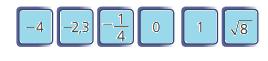
\includegraphics[width=2.79167in,height=0.63542in]{./imgSAEB_8_MAT/media/image1.png}
\end{figure}

Quais deles pertencem ao conjunto:


\begin{escolha}[itemsep=0pt]
\item N \rosa{'' $0; 1$}
\item Z \rosa{'' $-4, 0, 1$}
\item Z, mas não pertencem a N? \rosa{$-4$}
\item Q, mas não pertencem a Z? \rosa{$-2,3$ e  $(-\frac{1}{4})$}
\end{escolha}

\pagebreak

\num{4} Observe os números abaixo:

$$6; (\sqrt{6}); 6,6; -6$$


Identifique quais deles são:
\begin{escolha}[itemsep=0pt]
\item reais e naturais.\rosa{ -- 6}
\item reais e inteiros.\rosa{ -- 6 ; -6}
\item reais e racionais.\rosa{ -- 6; -6; 6,6}
\item reais e irracionais.\rosa{'' $(\sqrt{6})$}
\end{escolha}


\num{5} Complete os espaços abaixo com pertence ou não pertence:


\begin{multicols}{3}
\begin{enumerate}
\def\labelenumi{\alph{enumi}}
\item 100 
\item 100 
\item 100 
\item $(\sqrt{9}) 
$\item $(-\sqrt{9})$ 
\item $(\sqrt{- 9})$ 
\item 2,6 
\end{enumerate}


\begin{enumerate}
\item R*
\item R\textsubscript{+}
\item R\textsubscript{-}
\item R
\item R
\item R
\item R\textsubscript{+}
\end{enumerate}

\begin{enumerate}
\item \rosa{'' Pertence}
\item \rosa{'' Pertence}
\item \rosa{'' Não Pertence}
\item \rosa{'' Pertence}
\item \rosa{'' Pertence}
\item \rosa{'' Não Pertence}
\item \rosa{'' Pertence}
\end{enumerate}
\end{multicols}


\num{6} A representação decimal de um número pode ser: finita, infinita e
periódica ou, ainda, infinita e não periódica. Escreva qual é o caso de
cada um dos números a seguir

\begin{escolha}[itemsep=0pt]
\item $(\frac{15}{6})$ \rosa{'' Finita}
\item $(\frac{1}{3})$ \rosa{'' Infinita e periódica}
\item $(\sqrt{3})$ \rosa{'' Infinita e não periódica}
\item $(\sqrt{2})$ \rosa{'' Infinita e não periódica}
\end{escolha}


\num{7} O número $\pi$ é classificado como:
\reduline{ uma dízima não periódica.\hfill}\\

\num{8} O números $121$ é considerado um quadrado perfeito? Por quê?
\reduline{Sim, pois $121 = 11 \cdot 11$.\hfill}
\linhas{2}

\num{9} O produto ou o quociente de dois números irracionais pode ser um
número racional?

\reduline{ Sim, como exemplos podem ser citados\hfill}\\
\reduline{ $(\sqrt{2} \cdot \sqrt{2} = \sqrt{2}^2 = 2)$ e também $(\frac{\sqrt{2}}{\sqrt{2}} = 1)$\hfill}\\


\num{10} Qual é o menor número natural que devemos multiplicar pelo número
125 para que o produto seja um número quadrado perfeito?
\reduline{ $5$, pois $5\cdot 125 = 625$ e $(\sqrt{625}) = 25$.\hfill}\\

\section{Treino}

\num{1} Qual é a decomposição do número 1 000 em fatores primos?

\begin{escolha}[itemsep=0pt]
\item $(2^2\cdot 5^2)$
\item $(2^3 \cdot 5^2 \cdot 2)$
\item $(2^3 \cdot 5^3)$
\item $(2^3 \cdot 5^2)$
\end{escolha}



% SAEB: Compor ou decompor números racionais positivos (representação
% decimal finita) na forma aditiva, ou em suas ordens, ou em adições e
% multiplicações.

% A: Incorreta, pois, o aluno não computou um elemento $2$ e um elemento $5$
% na fatoração..

% B: Incorreta, pois o aluno computou um elemento a mais e um elemento $5$ a
% menos na fatoração.

% C: Correta, pois, ao decompor o número 1.000 em fatores primos, obtemos
% $2^3$ \cdot $5^3$.

% D: Incorreta, pois o aluno não computou um elemento 5 na fatoração.
% -----


\num{2} Sobre o número $123.456.789$, podemos afirmar que:

\begin{escolha}[itemsep=0pt]
\item é múltiplo de $5$
\item é múltiplo de $2$
\item é múltiplo de $3$
\item é múltiplo de $10$
\end{escolha}


% 2
% SAEB: Identificar um número natural como primo, composto,
% ``múltiplo/fator de'' ou ``divisor de'' ou identificar a decomposição de
% um número natural em fatores primos ou relacionar as propriedades
% aritméticas (primo, composto, ``múltiplo/fator de'' ou ``divisor de'')
% de um número natural à sua decomposição em fatores primos.

% A: Incorreta, pois o aluno pode realizar a divisão incorretamente do
% valor 123.456.789 e chegar a essa conclusão.

% B: Incorreta, pois o aluno pode realizar a divisão incorretamente do
% valor 123.456.789 e chegar a essa conclusão.

% C: Correta, pois (1 + 2 + 3 + 4 + 5 + 6 + 7 + 8 + 9 = 45). Logo, 45 é
% múltiplo de 3, então

% 123.456.789 também será.

% D: Incorreta, pois o aluno pode realizar a divisão incorretamente do
% valor $123.456.789$ e chegar a essa conclusão.
% ----

\num{3} Manoel ganhou um prêmio na loteria no valor de R\$\,12.500.345.769,00.
Qual algarismo está situado na casa da centena de milhar?

\begin{escolha}[itemsep=0pt]
\item $4$
\item $5$
\item $0$
\item $3$
\end{escolha}



%3
% SAEB: Compor ou decompor números racionais positivos (representação
% decimal finita) na forma aditiva, ou em suas ordens, ou em adições e
% multiplicações.

% A: Incorreta, pois, ao contar as casas erroneamente e considerar o
% número uma casa à direita o aluno pode considerar esse.

% B: Incorreta, pois, ao contar as casas erroneamente e considerar o
% número duas casas à direita, o aluno pode considerar esse resultado.

% C: Incorreta, pois, ao contar as casas erroneamente e considerar o
% número uma casa à esquerda, o aluno pode considerar esse resultado.

% D, Correta, pois o número 3 está situado na casa das centenas de milhar.
% ----

\chapter{Operações
aritméticas}

\section{Habilidades do SAEB}

\begin{itemize}
  \item Calcular o resultado de adições, subtrações,
multiplicações ou divisões envolvendo número reais.
\item
  Calcular o resultado de potenciação ou radiciação envolvendo números
  reais.
\item
  Resolver problemas de adição, subtração, multiplicação, divisão,
  potenciação ou radiciação envolvendo número reais, inclusive notação
  científica
\item
  Resolver problemas de contagem cuja resolução envolva a aplicação do
  princípio multiplicativo.
\item
  Resolver problemas que envolvam as ideias de múltiplo, divisor, máximo
  divisor comum ou mínimo múltiplo comum.
\end{itemize}

\subsection{Habilidades da BNCC}

\begin{itemize}
\item EF08MA01, EF08MA02, EF08MA03.
\end{itemize}

\conteudo{Dado um número racional a e um número natural n, a expressão ($a^n$)
chama-se potência e representa uma multiplicação de n fatores iguais ao
número a.

$$(a^n = \frac{a \cdot a \cdot a \cdot a \cdot a \cdot \ldots \cdot a}{n})$$
Essa operação é chamada potenciação.

Assim, pela definição, temos:

$$(10^3 = 10 \cdot 10 \cdot 10 = 1.000)$$

Propriedades da potenciação:

1ª. propriedade: Produto de potências de mesma base.

Um produto de potências de mesma base pode ser escrito na forma de uma
única potência: conservamos a base e adicionamos os expoentes.

$$(a^m) \cdot (a^n) = (a^{m+n})$$

2ª. Propriedade: Quociente de potências de mesma base

Um quociente de potências de mesma base, em que o expoente do dividendo
é maior ou igual ao expoente do divisor, pode ser escrito na forma de
uma única potência: conservamos a base e subtraímos os expoentes

$$(a^m) \div (a^n) = (a^{m-n})$$ 

com a diferente de zero e m maior ou
igual a n

3ª propriedade: Potência de uma potência.

Um produto de potências de mesma base pode ser escrito na forma de uma
única potência: conservamos a base e multiplicamos os expoentes.

$$(a^m)^n) = (a^{m \cdot n})$$

4ª. propriedade potência de um produto

Para elevar um produto de dois ou mais números racionais a um expoente,
elevamos cada fator a esse expoente.

$$((a \cdot b)^n)= (a^n x b^n)$$

A potência de base 10, com expoente natural, é uma maneira de se
escrever o número que, no Sistema de Numeração Decimal, é representado
por 1 seguido de n zeros.

$$(10^5 = 100.000 = 1 + 5...);$$
$$(10^5 = 100.000 = 1 + 5...)$$
$$(10^5 = 100.000 = 1 + 5...)$$

Se um número representa um produto de dois fatores iguais não negativos,
então cada fator é a raiz quadrada desse número. Por exemplo:

A raiz quadrada de 25 é 5, pois 

$$(10^5 = 100.000 = 1 + 5...)$$. 

Logo $(10^5 = 100.000 = 1 + 5)$.

A raiz quadrada de 49 é 7, pois:

 $$(10^5 = 100.000 = 1 + 5...)$$. 

 Logo $(\sqrt{49} = 7)$.}



\section{Atividades}

\num{1} Calcule o valor das potências abaixo.

\begin{escolha}[itemsep=0pt]
\item $\left( - \frac{3}{5}\right )^2$  \rosa{$(\frac{9}{25})$}
\item $( + \frac{1}{2}^5)$  \rosa{$(\frac{1}{32})$}
\item $( - 1\frac{1}{2}^3)$  \rosa{$\left(- \frac{3}{8}\right )$}
\item $( -3,5^2)$  \rosa{$+12,25$}
\item $( + \frac{1}{3}^0)$  \rosa{$1$}
\item $(-1,5^1)$  \rosa{$-1,5$}
\end{escolha}


\num{2} Calcule as operações abaixo.

\begin{escolha}[itemsep=0pt]
\item $(( - \frac{1}{2}^2 \; + \; -1^4)$ \rosa{ $(+ 1\frac{1}{4})$}
\item $ - (2^3 \cdot -2^3)$ \rosa{ $(+64)$}
\item $(( - 1\frac{1}{2} \cdot -1^5)$ \rosa{$(+ 1\frac{1}{2})$}
\item $\left ( - \frac{1}{2} \right) \cdot \left( + \frac{3}{2} \right) - \left ( \frac{2}{3} \right)^{3} / \left ( - \frac{1}{27}) \right)$  
    \rosa{$(8 \cdot \frac{3}{8})$}
\item $(0,1) ^2 / (-2) + (1,5) \cdot (-0,1)^2$ \rosa{$0,01$}
\end{escolha}







\num{3} Use a propriedade e, no caderno, escreva cada quociente como uma
única potência e calcule seu valor.


\begin{escolha}[itemsep=0pt]
\item $(3^7 \div 3^5)$ 
    \rosa{$(3^{7 - 5} = 3^2 = 3.3 = 9)$     }
\item $(-1^8:-1^6)$ 
    \rosa{$((-1^{8 - 6} = -1^2= -1\cdot-1= +1)$     }
\item $(\left( \frac{2}{3} \right) / \left ( \frac{2}{3} \right)$ 
    \rosa{$((\frac{2}{3})^{4-1}) = ((\frac{2}{3}))^3=(\ (\frac{2}{3}))\cdot(\ (\frac{2}{3}))\cdot(\ (\frac{2}{3})) = (\frac{8}{27})$      }
\item Metade de $(2^10)$ 
    \rosa{$(2^{10} / 2^1 = 2^9 = 2.2.2.2.2.2.2.2.2 = 572)$      }
\item $((-2,5)^5) \div (-2,5)^2$ 
    \rosa{$((-2,5)^{5-2} = (-2,5)^3= (-2,5). (-2,5). (-2,5) = -15,625)$     }
\item $(a^9 \div a^8)$, com a racional não nulo 
    \rosa{$(a^{9-8} = a^1 = a)    $  }
\item $(1^8 \div 1^2)$ 
    \rosa{$(1^{8-2} = 1^6= 1.1.1.1.1.1 = 1)$      }
\item terça parte de $(3^8)$ 
    \rosa{$(3^8-1)= (3^7) = 3.3.3.3.3.3.3 = 2187$     }
\end{escolha}



\num{4} Jamile fez uma viagem turística ao topo de uma montanha. Ao chegar em
certo local, observou uma pedra antiga com o seguinte enunciado: esta
pedra tem o peso de $[(-5)^3]^2\,kg$. Quanto pesa a pedra que Jandira
observou?

\reduline{ Utilizando a propriedade de multiplicação de expoentes temos que:\hfill}\\
\reduline{ $((-5)^{3.2}= (-5)^6= (-5) \cdot (-5) \cdot (-5) \cdot (-5) \cdot (-5) \cdot (-5)= 15.625 kg)$\hfill}\\


% -----------------

\num{5} Uma sala de jantar quadrada terá o piso coberto com ladrilhos com
medida de comprimento dos lados de 60 cm.


\begin{escolha}[itemsep=0pt]
\item Qual é a medida de comprimento dos lados da sala sabendo que a medida
de área dela é de $81 m^2$?
\item Quantos ladrilhos serão necessários para cobrir o piso?
\end{escolha}

\reduline{ (a) Considerando que a sala é quadrada e que a fórmula da área de um\hfill}\\
\reduline{ quadrado é $l^2$, para descobrirmos o real valor de cada lado, basta\hfill}\\
\reduline{ fazermos a operação inversa: $l^2 = 81; l= (\sqrt{81}); l= 9$\hfill}\\
\reduline{ (b) Se cada lado da sala possui 9 metros e cada lado do ladrilho possui 0,60 cm temos que:\hfill}\\
\reduline{ $9 \div 0,6 = 15;$ $(15 \cdot 15 = 225$ ladrilhos)\hfill}\\

\num{6} Utilizando os conhecimentos de redução de potências, reduza as
potencias abaixo.

\begin{escolha}[itemsep=0pt]
\item $10^2 \cdot 2^2$  
        \rosa{ $(10 \cdot 2)^2 = 20^2$ }
\item $11^2 \cdot 3^2$  
        \rosa{ $(11 \cdot 3)^2 = 33^2$ }
\item $(-6)^3 \cdot (-8)^3$  
        \rosa{ $((-6) \cdot (-8)) ^3 = 48^3$ }
\item $((3,1)^5 \cdot (0,7)^5 \cdot 2^5)$  
        \rosa{ $((3,1 \cdot 0,7 \cdot 2)^5= 4,34^5)$ }
\end{escolha}





\num{7} Calcule o valor de cada potência com exponente negativo

\begin{escolha}[itemsep=0pt]
\item $(8^{-2}$) 
              \rosa{$ (8^{-2} = \frac{1}{8^2}) = (\frac{1}{64})$}
\item $(5^{-1})$ 
              \rosa{$ 5^{-1}= (\frac{1}{5^1}) = (\frac{1}{5})$}
\item $((-2)^{-4}) $
              \rosa{$ ((-2)^{-4} = \frac{1}{2.4} = \frac{1}{16})$}
\item $((\frac{1}{2})^{-3}) $
              \rosa{$ ((\frac{1}{2})^{-3}) = (\frac{2}{1^3}) = (\frac{2}{1}) = 2$}
\item $((-3)^{-3}) $
              \rosa{$ ((-3)^{-3})= (\frac{1}{3^3}) = (\frac{1}{27})$}
\item $(\frac{1}{2}^{-5}) $
              \rosa{$ (\frac{1}{2}^{-5}) = (\frac{2}{1}^5) = 32$}
\end{escolha}


\num{8} Calcule as seguintes potências de base 10 e coloque-as em forma
decimal.

\begin{multicols}{2}
\begin{escolha}[itemsep=0pt]
\item $(10^6)$
    \rosa{$1 000 000$}
\item $(10^-6)$
    \rosa{$0, 000 001$}
\item $(10^-4)$
    \rosa{$0, 0001$}
\item $(10^4)$
    \rosa{$10 000$}
\item $(10^-2)$
    \rosa{$0,01$}
\item $(10 ^-5)$
    \rosa{$0,00001$}
\item $(10^10)$
    \rosa{$10 000 000 000$}
\item $(10^-8)$
    \rosa{$0,00000001$}
\end{escolha}
\end{multicols}

\num{9} Reinaldo é professor e, durante uma de suas aulas de estatística,
resolveu demonstrar a população da Terra em formato decimal. Porém, ao
tentar fazer a demonstração, o espaço de sua lousa não foi suficiente.
Sabendo que a população da Terra em 2022 chegou a 8 bilhões, como
poderíamos representar este número para que caiba na lousa?

\reduline{ Reinaldo poderia representar por meio de Notação científica (potência de base 10).\hfill}\\
\reduline{ Considerando a população da terra como 8.000.000.000, outra forma \hfill}\\
\reduline{ de reescrever seria $(8 \cdot 10^9)$.\hfill}\\

\num{10} Felipe é artista e uma de suas obras é conhecida como quadrado
infinito. Ao observar o quadro, um matemático fez as seguintes
descobertas:

\begin{multicols}{2}

\begin{figure}[H]
\centering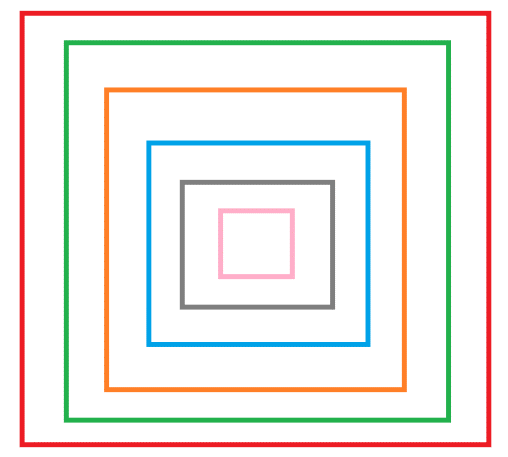
\includegraphics[width=2.3125in,height=2.07917in]{./imgSAEB_8_MAT/media/image2.png}
\end{figure}

\columnbreak

O quadrado Vermelho possui uma área de $25\,cm^2$.

O quadrado Verde possui uma área de $22\,cm^2$.

O quadrado Laranja possui uma área de $14\,cm^2$.

O quadrado Azul possui uma área de $64\,cm^2$.

O quadrado Cinza possui uma área de $36\,cm^2$.

O quadrado Rosa possui uma área de $16\,cm^2$.
\end{multicols}

Com as informações obtidas pelo matemático, responda às perguntas.

\begin{escolha}[itemsep=0pt]
\item Perímetro do quadrado vermelho.
        \rosa{  $(\sqrt{256} = 16, 16 \cdot 4 = perímetro = 64)$}
\item Perímetro do quadrado verde.
        \rosa{  $(\sqrt{225}) = 15, 15 \cdot 4 = perímetro = 60$}
\item Perímetro do quadrado laranja.
        \rosa{  $(\sqrt{144}) = 12, 12 \cdot 4 = perímetro= 48$}
\item Perímetro do quadrado azul.
        \rosa{  $(\sqrt{64}) = 8, 8 \cdot 4 = perímetro = 32$}
\item Perímetro do quadrado cinza.
        \rosa{  $(\sqrt{36}) = 6, 6 \cdot 4 = perímetro = 24$}
\item Perímetro do quadrado rosa.
        \rosa{  $(\sqrt{16}) = 4, 4 \cdot 4 = perímetro = 16$}
\end{escolha}

% \begin{figure}[H]
% \centering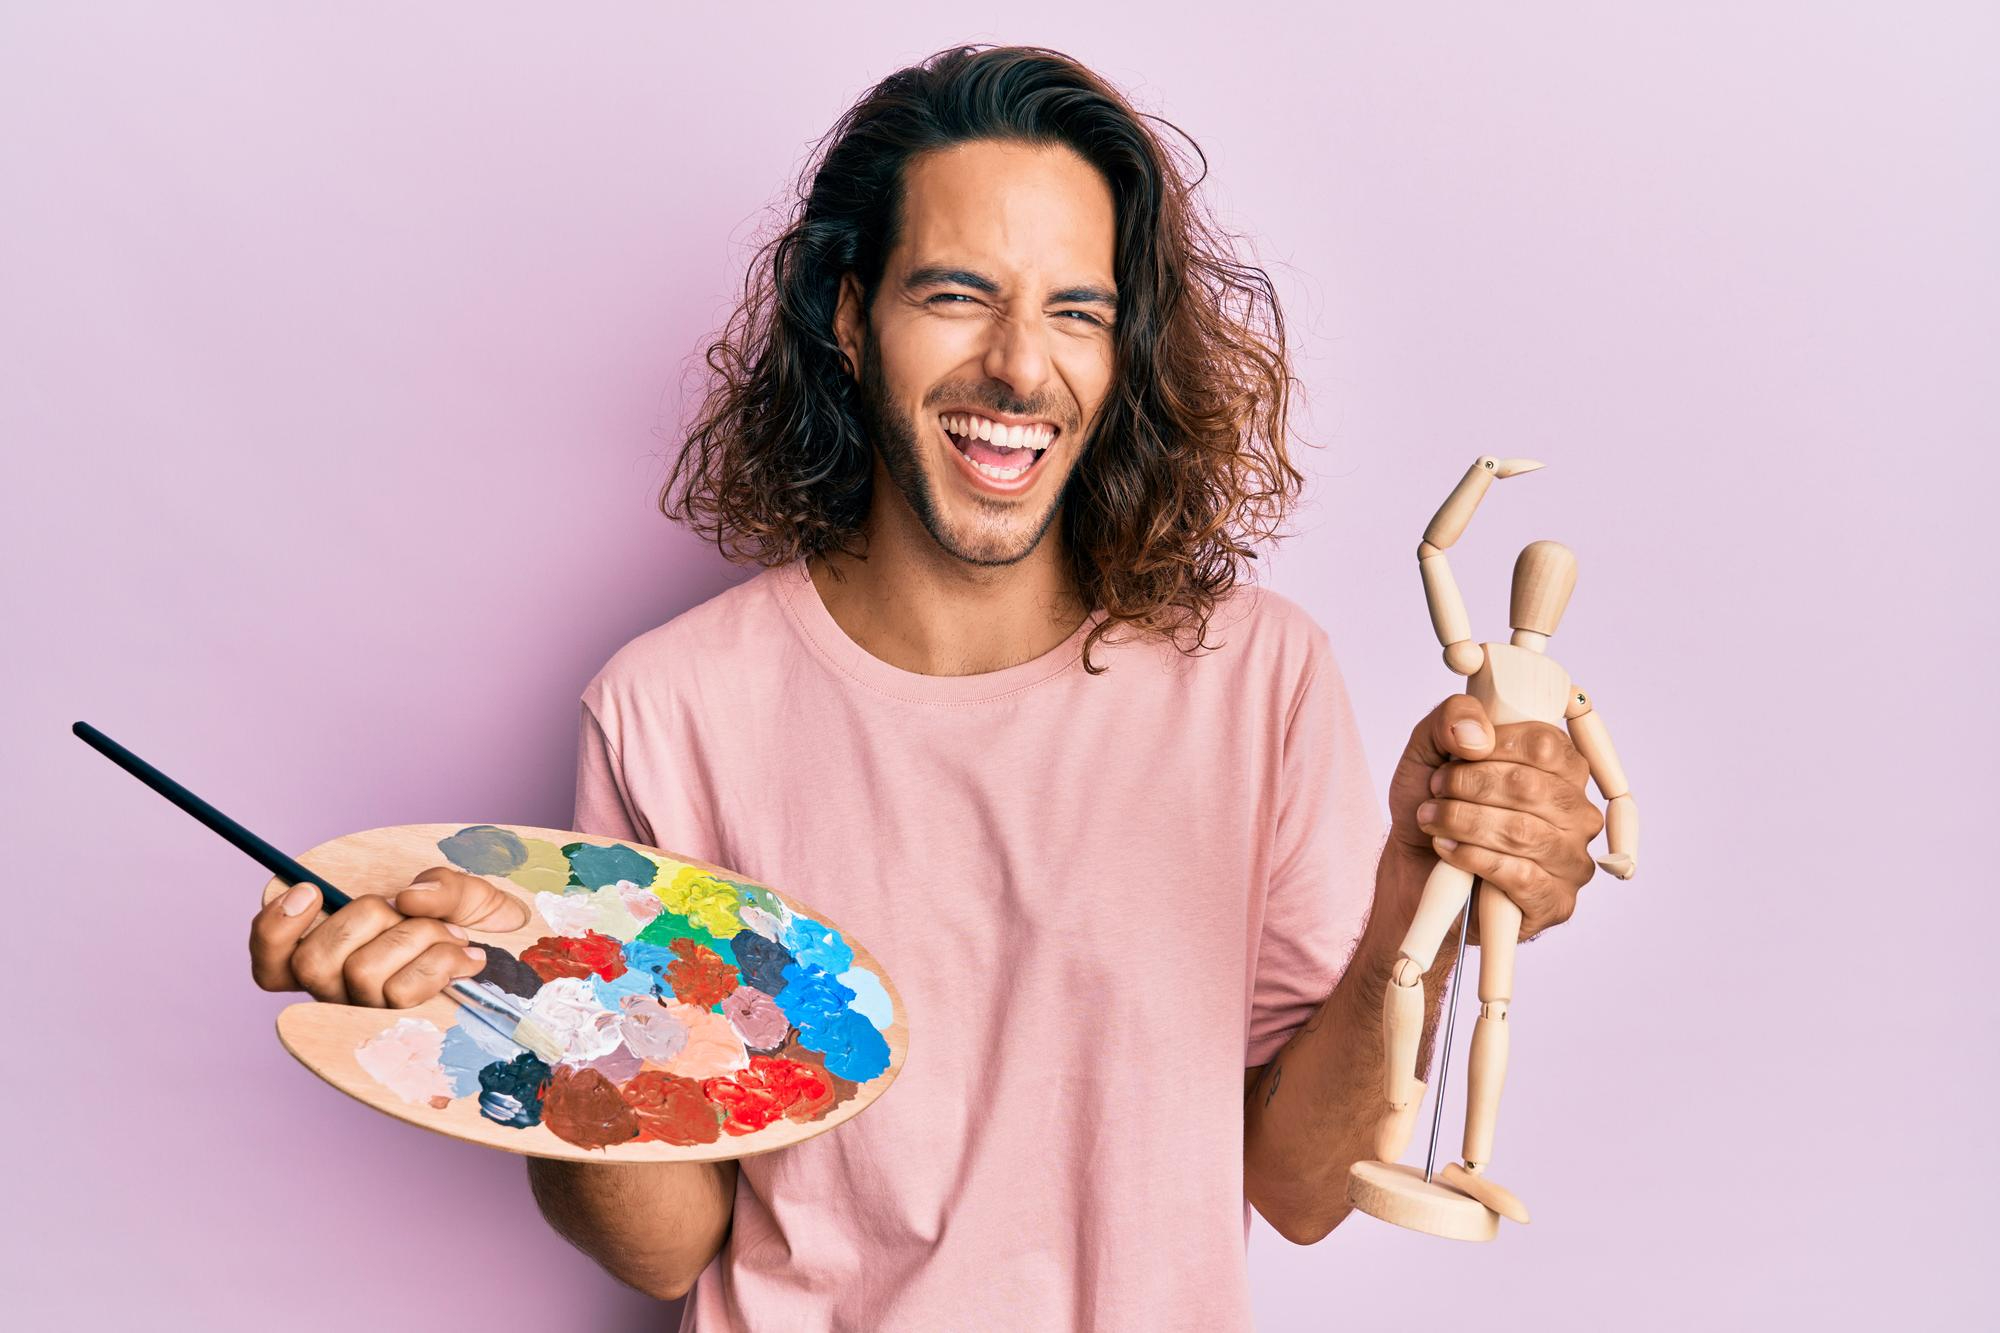
\includegraphics[width=\textwidth,keepaspectratio]{./imgSAEB_8_MAT/media/image63.png}
% \end{figure}
% \reduline{ Para descobrir o perímetro de cada quadrado a solução se mostra a mesma\hfill}
% \reduline{ se temos que a formula da área de um quadrado é l ^2 para descobrirmos o\hfill}
% \reduline{ real valor de cada lado, basta fazermos a operação inversa, no caso a radiciação.\hfill}

\pagebreak

\section{Treino}

\num{1} Raul estava passeando pela rua e, ao passar por uma loja de discos
antigos, viu um álbum com o seguinte título: ``Eu Nasci Há Dez Mil Anos
Atrás''. Se a capa desse álbum fosse representada em forma de potência
de base 10, qual o novo nome do álbum?

\begin{escolha}[itemsep=0pt]
\item Eu Nasci Há $10^2$ anos Atrás
\item Eu Nasci Há $10^3$ anos atrás
\item Eu Nasci Há $10^4$ anos atrás
\item Eu Nasci Há $10^5$ Anos Atrás
\end{escolha}


% SAEB: Resolver problemas de adição, subtração, multiplicação, divisão,
% potenciação ou radiciação envolvendo número reais, inclusive notação
% científica

% BNCC: EF08MA02 -- Resolver e elaborar problemas usando a relação entre
% potenciação e radiciação, para representar uma raiz como potência de
% expoente fracionário.

% A: Incorreta, pois o número de zeros estava errado.

% B: Incorreta, pois o número de zeros estava errado.

% C: Correta, pois:

% $10000 = 10 \cdot 10 \cdot 10 \cdot 10$ ou seja $(10^4)$

% D: Incorreta, pois o número de zeros estava errado.

\num{2} Thiago é um professor de matemática e, ao comemorar seu aniversário
com seus alunos, resolveu lançar um enigma. Sua idade seria o expoente
do resultado da seguinte expressão:

$$(\frac{2^{25} \cdot 2^{35} \cdot 2^{30}} {2^2.2^1})$$

Qual é a Idade de Thiago?

\begin{escolha}[itemsep=0pt]
\item 2
\item 93
\item 45
\item 30
\end{escolha}

% SAEB: Resolver problemas de adição, subtração, multiplicação, divisão,
% potenciação ou radiciação envolvendo número reais, inclusive notação
% científica

% A: Incorreta, pois, ao confundir expoente com base, o aluno chegaria a
% esse resultado.

% B: Incorreta, pois o aluno chegaria a esse conclusão se somasse todos os
% expoentes incorretamente.

% C: Incorreta, pois, ao dividir o expoente do numerador por 2 ao invés de
% 3, o aluno chegaria a esse resultado.

% D: Correta pois, utilizando a propriedade de multiplicação e divisão de
% potências de mesma base, temos que

% No numerador $(2^{25+35+30}=2^{90})$.

% No denominador $(2^{2+1}) = 2^3$.

% Realizando a divisão, temos que $(2^{90}:3) = (2^{30})$.

% Considerando que a idade de Thiago é apenas o expoente, sabemos que
% Thiago tem 30 anos.

\num{3} Um pen drive possui diferentes capacidades de memória, mas a medida
normalmente utilizada é o GB. Sabendo que 1 GB = $(2^{10})$ megabytes,
ao comprar um pen drive de 32 GB, quantos megabytes de armazenamento
estarão disponíveis?

\begin{escolha}[itemsep=0pt]
\item 32.768 megabytes
    \rosa{ Correta, pois: $(2^10) = 1024$; $1024 \cdot 32 = 32.768$ megabytes.}
\item 32.000 megabytes
    \rosa{ Incorreta, o aluno chegaria a esse resultado ao considerar que $(2^{10})$ seja 1.000 ao invés de 1.024.}
\item 16.384 megabytes
    \rosa{ Incorreta, pois, ao considerar um 2 a menos na expressão, o aluno chegaria a esse resultado.}
\item 64 megabytes
    \rosa{ Incorreta, pois, ao realizar apenas a multiplicação ao\\ invés de realizar o cálculo da potência, o aluno chegaria a esse resultado.}
\end{escolha}


% SAEB: Resolver problemas de adição, subtração, multiplicação, divisão,
% potenciação ou radiciação envolvendo número reais, inclusive notação
% científica.

% BNCC: EF08MA01 -- Efetuar cálculos com potências de expoentes inteiros e
% aplicar esse conhecimento na representação de números em notação
% científica.



\chapter{Frações}

\section{Habilidades do SAEB}

\begin{itemize}
\item
  Identificar frações equivalentes.
\item
  Determinar uma fração geratriz para uma dízima periódica.
  \item Representar frações menores ou maiores que a
unidade por meio de representações pictóricas ou associar frações a
representações pictóricas.
\end{itemize}

\subsection{Habilidade da BNCC}

\begin{itemize}
  \item EF08MA051.
\end{itemize}

\conteudo{
\smallskip\noindent\textbf{Comparação de números racionais}\quad
Comparar dois números racionais significa estabelecer se entre eles
existe uma relação de superioridade, inferioridade ou igualdade.

Todo número racional negativo é menor que todo número racional positivo

$$(\frac{1}{5} \textless \frac{3}{4})$$

Todo número racional negativo é menor que zero. $-5 \textless{} 0 -12,5 \textless{} 0 -(\frac{3}{2}) \textless{} 0$

\smallskip\noindent\textbf{Operações com números racionais: adição e subtração}\quad
Na forma fracionária, temos que estudar dois casos distintos: o primeiro
deles refere-se às frações com denominadores iguais.

O segundo, às frações com denominadores diferentes.

1º. caso: Frações de mesmo denominador.

Para somarmos (ou subtrairmos) frações de mesmo denominador, mantemos o
denominador e somamos (ou subtraímos) os numeradores. Veja um exemplo:

$$(\frac{3}{5}) + (\frac{6}{5}) = (\frac{9}{5})$$

2° caso: Frações com denominadores diferentes.

Para somarmos (ou subtrairmos) frações com denominadores diferentes,
devemos obter frações equivalentes às frações dadas, de mesmo
denominador. Em seguida, mantemos o denominador comum e somamos (ou
subtraímos) os numeradores.

$$(\frac{2}{4}) + (\frac{3}{7}) = (\frac{14 + 12}{28}) = (\frac{26}{28})$$

\smallskip\noindent\textbf{Multiplicação de números racionais}\quad
Para multiplicarmos dois números racionais na forma fracionária,
multiplicamos os numeradores entre si e, em seguida, os denominadores.
Caso seja necessário, simplificamos o resultado até obter a fração
irredutível. Exemplo:

$$(\frac{3}{4}) \cdot (\frac{2}{5}) = (\frac{6}{20})= (\frac{3}{10})$$

\smallskip\noindent\textbf{Divisão de números racionais}\quad
Para dividirmos dois números racionais na forma fracionária, mantemos a
primeira fração e multiplicamos pelo inverso da segunda.

$$(\frac{1}{2}) \div (\frac{3}{5})= (\frac{1}{2}) \cdot (\frac{5}{3}) = (\frac{5}{6})$$

\smallskip\noindent\textbf{Dízimas periódicas}\quad
Em Matemática, muitas vezes, é útil representar números racionais,
expressos por meio de frações, na forma decimal. Para isso, basta
dividir o numerador pelo denominador. Em alguns casos, essa
representação decimal é finita. Já em outros casos, ela é infinita.
Exemplo:

$$(\frac{1}{3}) = 0,3333333......$$

\smallskip\noindent\textbf{Fração geratriz de dízimas periódicas simples}\quad
Vamos encontrar a fração geratriz da dízima periódica $0,333333...$, ou
seja, encontrar qual fração, quando transformada em número racional na
forma decimal, gera essa dízima.

Para isso, montamos uma equação:
$$0,333333333... - x$$
$$3,33333333... - 10x$$
$$3,3333333333... - 0,333333333... = 3$$
$$10x - x = 9x$$

Logo temos que $(\frac{3}{9})$ simplificando $(\frac{1}{3})$ é a nossa
fração geratriz.
}



\section{Atividades}

\num{1} Classifique com V para verdadeiro e F para falso as afirmações a
seguir:

\begin{boxlist}
\boxitem{F} $4,9 = 4,09$
    \rosa{$ 4,9 = 4,09$}
\boxitem{V} $-15,3 \textless{} 15,3$
    \rosa{$ -15,3 \textless{} 15,3$}
\boxitem{F} $(\frac{19}{3}) \textgreater{} (\frac{23}{3})$
    \rosa{$ (\frac{19}{3}) \textgreater{} (\frac{23}{3})$}
\boxitem{V} $(-\frac{89}{7}) \textless{} \left(- \frac{63}{4}\right )$
    \rosa{$ (-\frac{89}{7}) \textless{} \left(- \frac{63}{4}\right )$}
\boxitem{F} $\left(- \frac{7}{5}\right ) \textgreater{} -1,4$
    \rosa{$ \left(- \frac{7}{5}\right ) \textgreater{} -1,4$}
\boxitem{V} $23,98 \textgreater{} 23,89$
    \rosa{$ 23,98 \textgreater{} 23,89$}
\end{boxlist}



\num{2} Efetue as operações a seguir:


\begin{escolha}[itemsep=0pt]
\item $\left(- \frac{8}{5}\right ) + 2,5 =$
        \rosa{$ \left(- \frac{8}{5}\right ) + 2,5 = -(\frac{8}{5}) + (\frac{25}{10}) = (\frac{- 16}{10})+(\frac{25}{10}) = (\frac{9}{10})$}
\item $(\frac{14}{3}) + (\frac{19}{5})$
        \rosa{$ (\frac{14}{3}) + (\frac{19}{5})= (\frac{70}{15}) + (\frac{57}{15}) = (\frac{127}{15})$}
\item $-(\frac{8}{13}) - (\frac{3}{5})$
        \rosa{$ (-\frac{8}{13}) - (\frac{3}{5}) = ( -\frac{40}{65}) - (\frac{39}{65}) = (-\frac{79}{65})$}
\item $79,02 - (\frac{12}{5})$
        \rosa{$ 79,02 - (\frac{12}{5}) = (\frac{7.902}{100}) - (\frac{12}{5}) = (\frac{7.902}{100}) - (\frac{240}{100}) = (\frac{7.662}{100})$}
\item $125 - (\frac{35}{4})$
        \rosa{$ 125 - (\frac{35}{4}) = (\frac{125}{1}) - (\frac{35}{4}) = (\frac{500}{4}) - (\frac{35}{4}) = (\frac{465}{4})$}
\item $(\frac{49}{7}) + (\frac{2}{3})$
        \rosa{$ (\frac{49}{7}) + (\frac{2}{3}) = (\frac{147}{21}) + (\frac{14}{21}) = (\frac{161}{21})$}
\item $50 - (\frac{1}{2})$
        \rosa{$ 50 - (\frac{1}{2}) = (\frac{50}{1}) - (\frac{1}{2}) = (\frac{100}{2}) - (\frac{1}{2}) = (\frac{99}{2})$}
\item $100 - (\frac{1}{3})$
        \rosa{$ 100 - (\frac{1}{3}) = (\frac{100}{1}) - (\frac{1}{3}) = (\frac{300}{3}) - (\frac{1}{3}) = (\frac{299}{3})$}
\end{escolha}







\num{3} Resolva as multiplicações abaixo, mas antes de calculá-las,
transforme os decimais em números fracionários.

\begin{escolha}[itemsep=0pt]
\item $0,5 \cdot 12,7$ 
        \rosa{ $0,5 \cdot 12,7 = (\frac{5}{10}) \cdot (\frac{127}{10}) = (\frac{635}{100})$}
\item $3,6 \cdot 6,7$ 
        \rosa{ $3,6 \cdot 6,7 = (\frac{35}{10}) \cdot (\frac{67}{10})$}
\item $9,3 \cdot 13,25$ 
        \rosa{ $9,3 \cdot 13,25 = (\frac{93}{10}) \cdot (\frac{1325}{100}) = (\frac{123\ 225}{1\ 000})$}
\item $2,9 \cdot 3,8$ 
        \rosa{ $2,9 \cdot 3,8 = (\frac{29}{10}) \cdot (\frac{38}{10}) = (\frac{1102}{100})$}
\item $11,2 \cdot 4,2$ 
        \rosa{ $11,2 \cdot 4,2= (\frac{112}{10}) \cdot (\frac{42}{10}) = (\frac{4\ 704}{100})$}
\item $7,5 \cdot 6,6$ 
        \rosa{ $7,5 \cdot 6,6 = (\frac{75}{10}) \cdot (\frac{66}{10}) = (\frac{4950}{100})$}
\item $0,456 \cdot 0,345$ 
        \rosa{ $0,456 \cdot 0,345 = (\frac{456}{1\ 000}) \cdot (\frac{345}{1\ 000}) = (\frac{157\ 320}{1\ 000\ 000})$}
\item $0,01 \cdot 0,001$ 
        \rosa{ $0,01 \cdot 0,001= (\frac{1}{100}) \cdot (\frac{1}{1\ 000}) = (\frac{1}{100\ 000})$}
\end{escolha}

\pagebreak

\num{4} Resolva as divisões abaixo, mas antes transforme os decimais em
números fracionários.

\begin{escolha}[itemsep=0pt]
\item $0,5 \div 3,4$
        \rosa{ $0,5 \div 3,4 = (\frac{5}{10}) \div (\frac{34}{10}) = (\frac{5}{10}) \cdot (\frac{10}{34}) = (\frac{50}{340})$}
\item $9,4 \div 3,1$
        \rosa{ $9,4 \div 3,1 = (\frac{94}{10}) \div (\frac{31}{10}) = (\frac{94}{10}) \cdot (\frac{10}{31}) = (\frac{940}{310})$}
\item $5,1 \div 0,2$
        \rosa{ $5,1 \div 0,2 = (\frac{51}{10}) \div (\frac{2}{10}) = (\frac{51}{10}) \cdot (\frac{10}{2}) = (\frac{510}{20})$}
\item $0,2 \div 0,1$
        \rosa{ $0,2 \div 0,1 = (\frac{2}{10}) \div (\frac{1}{10}) = (\frac{2}{10}) \cdot (\frac{10}{1}) = (\frac{20}{10}) = 2$}
\item $0,01 \div 0,001$
        \rosa{ $0,01 \div 0,001= (\frac{1}{100}) \div (\frac{1}{1\ 000}) = (\frac{1}{100}) \cdot (\frac{1\ 000}{1}) = (\frac{1\ 000}{100}) = 10$}
\item $2,1 \div 0,5$
        \rosa{ $2,1 \div 0,5 = (\frac{21}{10}) \div (\frac{5}{10}) = (\frac{21}{10}) \cdot (\frac{10}{5}) = (\frac{210}{50})$}
\item $4,2 \div 0,1$
        \rosa{ $4,2 \div 0,1 = (\frac{42}{10}) \div (\frac{1}{10}) = (\frac{42}{10}) \cdot (\frac{10}{1}) = (\frac{420}{10}) = 42$}
\item $3,1: 1,5$
        \rosa{ $3,1: 1,5 = (\frac{31}{10}) \div (\frac{15}{10}) = (\frac{31}{10}) \cdot (\frac{10}{15}) = (\frac{310}{150})$}
\end{escolha}



\num{5} Transforme as dízimas periódicas abaixo em frações geratrizes:

\begin{escolha}[itemsep=0pt]
\item $2,333333...$
        \rosa{$ (\frac{21}{9}) = (\frac{7}{3})$}
\item $3,181818...$
        \rosa{$ (\frac{315}{99})$}
\item $0,144444...$
        \rosa{$ (\frac{13}{90})$}
\item $4,166666...$
        \rosa{$ (\frac{375}{90}) = (\frac{25}{6})$}
\item $1,2222...$
        \rosa{$ (\frac{11}{9})$}
\end{escolha}


\num{6} Prove que $0,99999999999999 = 1$

\reduline{ $(\frac{0,99999999}{9,99999999} = \frac{x}{10x})$\hfill}\\
\reduline{ $9,999999999 -- 0,999999999 = 9;  10 x - x = 9$ \hfill}\\
\reduline{ Logo $(\frac{9}{9}) = 1$\hfill}\\

% \num{7} Complete com X as lacunas corresponde aos valores corretos

% %Paulo: criar uma tabela com os valores abaixo:
% \begin{figure}[H]% 
% \centering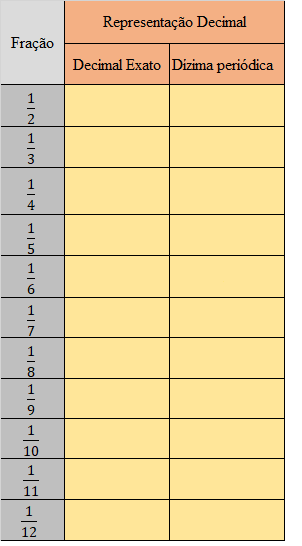
\includegraphics[width=2.37378in,height=4.29167in]{./imgSAEB_8_MAT/media/image3.png}
% \end{figure}

% %Paulo: criar uma tabela com os valores abaixo:
% \begin{figure}[H]% 
% \centering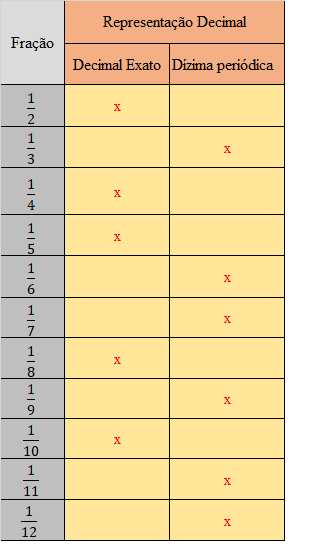
\includegraphics[width=2.14722in,height=3.775in]{./imgSAEB_8_MAT/media/image4.png}
% \end{figure}

\num{7} Ao realizar duas operações na calculadora, Juliana obteve os
seguintes resultados: 3,33333333... e 0,8888888...

Quais operações Juliana pode ter realizado?

\reduline{ $(\frac{3,333333333}{33,33333333} = \frac{x}{10x})$\hfill}\\
\reduline{ $33,33333333... - 3,33333333... = 30$\hfill}\\
\reduline{ $10 x - x = 9$; Logo, temos que Juliana chegou à fração $(\frac{30}{9})$\hfill} \\
\reduline{ ou equivalentes. Analogamente, temos que\hfill}\\
\reduline{ $(\frac{0,888888888}{8,888888888} = \frac{x}{10x}) 8,8888888... -- 0,88888888 = 8; 10x - x = 9$\hfill}\\
\reduline{ Logo, temos que Juliana chegou à fração $(\frac{8}{9})$, ou equivalentes.}\\



\num{8} Um professor de matemática aposentado resolveu inovar em sua festa de
aniversário. Na parede do salão de festas, colocou um cartaz com os
seguintes dizeres ``ao descobrirem a fração geratriz do número
5,454545..., saberão que o numerador desta fração é a idade que estou
completando hoje''. Quantos anos o professor está completando?

\reduline{$5,45454545... \longrightarrow x$\hfill}\\
\reduline{$545,454545... \longrightarrow 100x$\hfill}\\
\reduline{$(\frac{5,45454545}{545,454545} = \frac{x}{100x})$\hfill}\\
\reduline{$5,45454545... - 545,454545 = 540; 100 - x = 99$\hfill}\\
\reduline{Logo temos que $(\frac{540}{99}) = (\frac{60}{11})$, logo, 60 anos.}\\



\num{9} Marly e João são irmãos gêmeos. Ao divirem tarefas domésticas,
decidiram que cada um ia limpar uma parte da casa, desde que ambos
limpassem ao final a mesma fração que o outro. Sabendo que Marly limpou
$(\frac{3}{9})$ da casa, qual fração João deverá limpar?

\reduline{ O aluno pode responder qualquer fração equivalente, tal como $(\frac{6}{18})$.\hfill}\\

\section{Treino}

\num{1} Assinale a alternativa correta:

\begin{escolha}[itemsep=0pt]
\item O valor do número $(\pi)$ é aproximadamente
$3,14159265358979323846$\ldots, e ele é considerado uma dízima periódica
simples, pois seus 3 últimos números são pares.
\item O número de ouro representado pelo número $1.61803399$... é considerado
uma dízima periódica simples.
\item Ao calcularmos uma dízima periódica simples, sempre encontramos uma
fração geratriz.
\item O conjunto dos números irracionais é composto por dízimas periódicas
simples.
\end{escolha}

% SAEB: Determinar uma fração geratriz para uma dízima periódica.

% BNCC: EF08MA05 -- Reconhecer e utilizar procedimentos para a obtenção de
% uma fração geratriz para uma dízima periódica.

% A: Incorreta, pois o aluno pode considerar que o número (\pi) seja de
% fato uma dízima periódica simples pelo fato de ter números pares na sua
% composição.

% B: Incorreta, pois o aluno pode não conhecer a diferença entre uma
% dízima periódica simples e uma irracional.

% C: Correta, pois o conceito foi descrito corretamente.

% D: Incorreta, pois o aluno pode não ser capaz de identificar a diferença
% entre uma dizima periódica simples e uma irracional.

\num{2} Ao realizar uma palestra, um renomado médico descobriu que apenas
$(\frac{2}{3})$ dos convidados se consultava regularmente. Tendo em
vista que compareceram 300 pessoas ao evento, quantos participantes não
costumam se consultar?

\begin{escolha}[itemsep=0pt]
\item 200
\item 150
\item 600
\item 100
\end{escolha}

% SAEB: Representar frações menores ou maiores que a unidade por meio de
% representações pictóricas ou associar frações a representações
% pictóricas.

% BNCC: EF08MA05 -- Reconhecer e utilizar procedimentos para a obtenção de
% uma fração geratriz para uma dízima periódica.

% A: Incorreta, pois esse valor corresponde a $(\frac{2}{3})$ dos
% participantes.

% B: Incorreta, pois esse valor corresponde à metade dos participantes.

% C: Incorreta, pois esse valor corresponde ao dobro dos partcipantes.

% D: Correta, pois $(\frac{1}{3})$ de 300 é igual a 100.



\num{3} Ao fazer um bolo de aniversário, Cecilia utiliza 400\,g de farinha de
trigo. Ao dividir este bolo em 22 pedaços, qual fração geratriz
representara a quantidade de farinha em cada pedaço de bolo?

\begin{escolha}[itemsep=0pt]
\item $(\frac{200}{1})$ 
\item $(\frac{1000}{99})$ 
\item $(\frac{200}{9})$ \rosa{(X)}
\item $(\frac{1800}{101})$ 
\end{escolha}

\begin{figure}[H]
\centering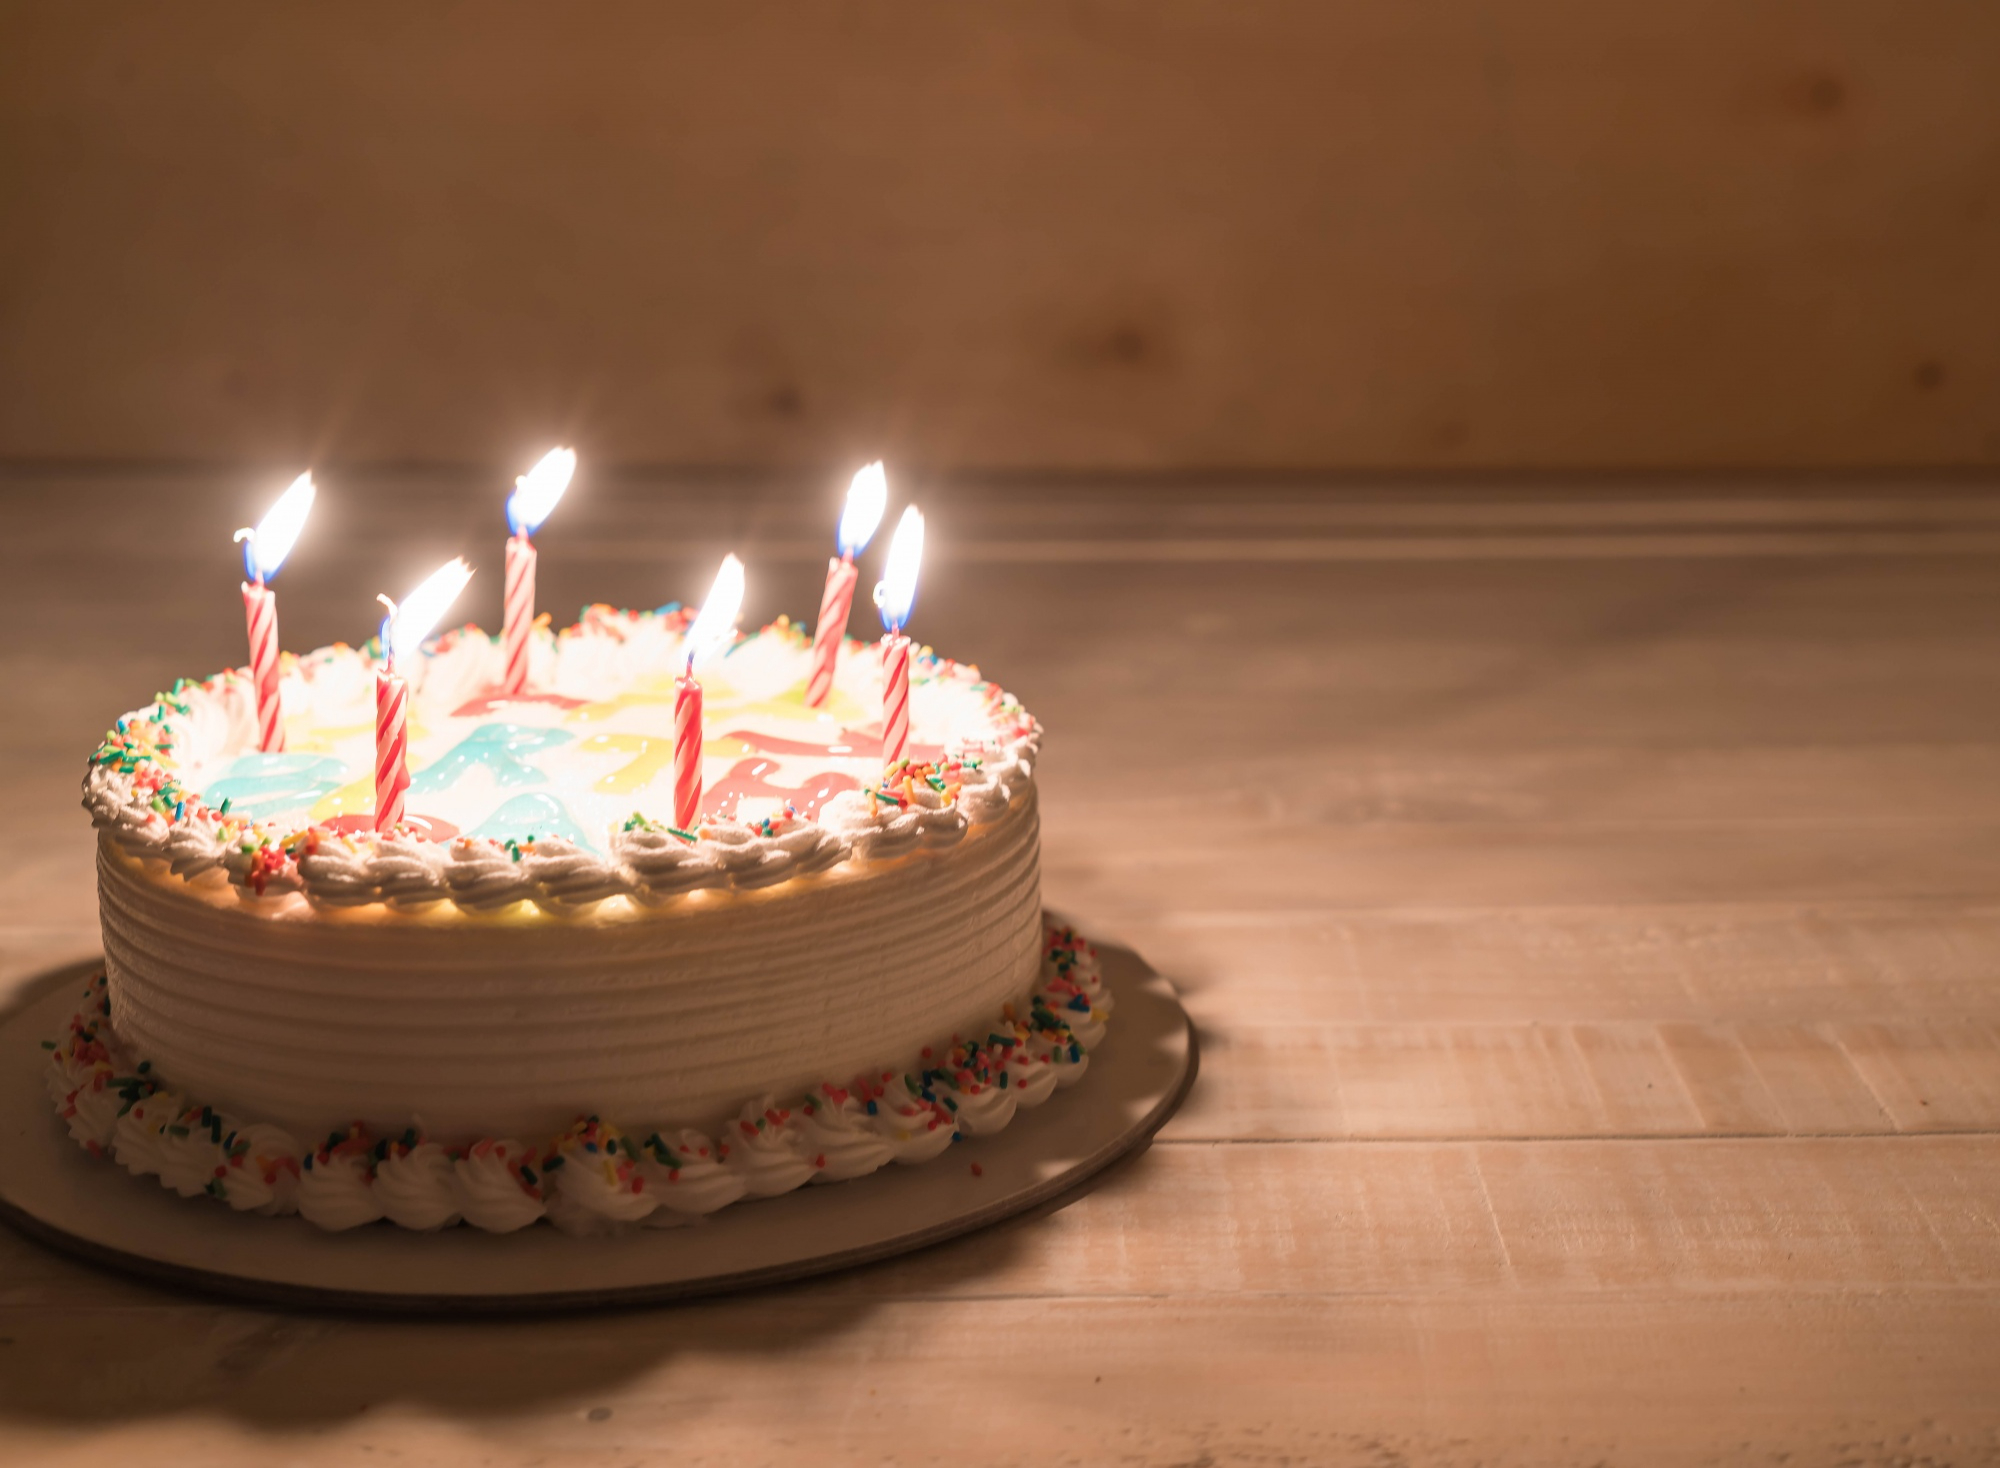
\includegraphics[width=\textwidth,keepaspectratio]{./imgSAEB_8_MAT/media/image64.png}
\end{figure}

% SAEB: Determinar uma fração geratriz para uma dízima periódica.

% BNCC: EF08MA05 -- Reconhecer e utilizar procedimentos para a obtenção de
% uma fração geratriz para uma dízima periódica.

% A: Incorreta, pois o aluno pode chegar a esse valor ao calcular
% erroneamente a expressão.

% B: Incorreta, pois o aluno pode chegar a esse valor ao calcular
% erroneamente a expressão.

% C: Correta, pois: 400 g \div 22 pedaços = 18,1818181818.\ldots{}

% 18,181818181818...
% -\/-\/-\/-\/-\/-\/-\/-\/-\/-\/-\/-\/-\/-\/-\/-\/-\/-\/-\/- x

% 1818,18181818...
% -\/-\/-\/-\/-\/-\/-\/-\/-\/-\/-\/-\/-\/-\/-\/-\/-\/-\/-\/-\/-\/-\/-100x

% (\frac{18,181818181818}{1818,18181818} = \frac{x}{100x})

% 1818,181818.\ldots{} - 18,18181818... = 1800

% 100x - x = 99x

% Logo, temos (\frac{1\ 800}{99}). Dividindo ambos por 9, temos que
% (\frac{200}{9}).

% D \div Incorreta, pois o aluno pode chegar a esse valor ao calcular
% erroneamente a expressão.


\chapter{Porcentagens}

\section{Habilidade do SAEB} 

\begin{itemize}
\item Resolver problemas que envolvam porcentagens,
incluindo os que lidam com acréscimos e decréscimos simples, aplicação
de percentuais sucessivos e determinação de taxas percentuais.
\end{itemize}

\subsection{Habilidade da BNCC}

\begin{itemize}
\item EF08MA04.
\end{itemize}



\conteudo{Porcentagem é a divisão por cem de algo a ser calculado. 


Podemos calcular pelo método da regra
de 3 simples ou pelo método multiplicativo de seu corresponde decimal.

Exemplo: $$25\% de 300$$

Pelo método da regra de três simples, temos:

$$\frac{100\%}{25\%} \cdot \frac{300}{x}$$
$$100x = 25 \cdot 300$$
$$100x = 7500$$
$$x = 75$$

Pelo método multiplicativo de seu correspondente decimal, temos:

$$300 \cdot (\frac{25}{100}) = 75$$}



\pagebreak


\section{Atividades}

\num{1} Em uma gincana realizada por uma escola, haverá várias modalidades
para os alunos. Ao final das inscrições, 30 alunos escolheram jogar
futsal, 18 alunos escolheram jogar Vôlei, 45 alunos escolheram jogar
basquete e 32 alunos escolheram não participar de nenhuma modalidade.

Calcule então:

\begin{escolha}[itemsep=0pt]
\item \% dos alunos que escolheram jogar futsal.\\
\rosa{$ (\frac{125}{30} = \frac{100}{x}); 125 \cdot x = 30 \cdot 100; 125x = 3000; x = 24 \%$}
\item \% dos alunos que escolheram jogar vôlei.\\
\rosa{$ (\frac{125}{18} = \frac{100}{x}); 125 \cdot x = 100 \cdot 18; 125x = 1800; x = 14,4\%$}
\item \% dos alunos que escolheram jogar basquete.\\
\rosa{$ (\frac{125}{45} = \frac{100}{x}); 125 x = 4500; x = 36\%$}
\item \% dos alunos que escolheram não participar de nenhuma modalidade.\\
\rosa{$ (\frac{125}{32} = \frac{100}{x}); 125 \cdot x = 32 \cdot 100; 125x = 3200; x = 25,6\%$}
\end{escolha}

Em cada item acima deixar o espaço de 3 linhas para resposta.






\num{2} Marcos é corretor de imóveis. Em janeiro, após ter um grande sucesso
em suas vendas, ele recebeu um aumento de 10\% no salário, que passou a
ser de R\$\,2.178,00. O valor do salário de Marcos antes do aumento era:

\begin{escolha}[itemsep=0pt]
\item R\$\,1.980,00
\item R\$\,1.990,00
\item R\$\,2.000,00
\item R\$\,2.100,00
\end{escolha}


%Deixar o espaço de 3 linhas para resposta.

\reduline{ Utilizando a regra de 3 simples, temos que:\hfill}\\
\reduline{$ (\frac{x}{2178} = \frac{100}{110}); Logo, x \cdot 110 = 2178 \cdot 100; 110x = 217 800; x = 1980$\hfill}\\

\num{3} Após uma apresentação de teatro, 250 espectadores foram entrevistados
e opinaram sobre o show. Veja o resultado dessa pesquisa:

\begin{itemize}
\item
  Ótimo = 105
\item
  Bom = 100
\item
  Regular = 30
\item
  Ruim = 15
\end{itemize}

Calcule a porcentagem de cada opinião.

\reduline{ Ótimo: $(\frac{250}{105} = \frac{100}{x}); 250 \cdot x = 100 \cdot 105; 250x = 10 500; x = 42\%$ \hfill}\\
\reduline{ Bom: $(\frac{250}{100} = \frac{100}{x})$\hfill}\\
\reduline{ $250 \cdot x = 100 \cdot 100; 250x= 10 000; x = 40\%$\hfill}\\
\reduline{ Regular: $(\frac{250}{30} = \frac{100}{x}); 250.x=100 .30; 250x = 3000; x = 12\%;$ \hfill}\\
\reduline{ $(\frac{250}{15} = \frac{100}{x}); 250x = 100 \cdot 15; 250 x = 1500; x = 6\%$\hfill}\\
\linhas{2}

\num{4} Valdemar é mecânico e adquiriu um carro quebrado pelo valor de
R\$\,10.000,00. Depois que o consertou, resolveu vendê-lo. Ele anunciou o
carro pelo valor de R\$\,16.000,00. Qual é o fator multiplicativo que ele
utilizou?

\reduline{ Utilizando a regra de 3 simples temos que:\hfill}\\
\reduline{ $(\frac{10.000}{16.000} = \frac{100}{x})$\hfill}\\
\reduline{ Logo $10.000 \cdot x = 16.000 \cdot 1.000$\hfill}\\
\reduline{ $10.000x = 1.600.000; x = 160$\hfill}\\

Logo houve um acréscimo de 60\%, então 60 \div 100 = 0,6.

O fator multiplicativo foi de 0,6.

\num{5} Amanda trabalha em uma loja de calçados. Certo dia, seu gerente
ofereceu uma porcentagem fixa de comissão para cada funcionário.para as vendas de
um tênis de 150 reais Amanda obteve uma comissão de 12 reais. Qual porcentagem
fixa Amanda ganhará sobre cada produto?

\reduline{ Utilizando a regra de 3 simples, temos que:\hfill}\\
\reduline{ $(\frac{150}{12} = \frac{100}{x})$\hfill}\\
\reduline{ Logo 150 \cdot x = 12 \cdot 100; 150 x = 1.200; x = 8 \%\hfill}\\

\num{6} Em um colégio, estudam 3.200 alunos, dos quais 1.440 são meninos. O
número de meninas representa quantos por cento do total de alunos que estudam
nesse colégio?

\reduline{ Utilizando a regra de 3 simples temos que:\hfill}\\
\reduline{ $(\frac{3.200}{1.440} = \frac{100}{x})$\hfill}\\
\reduline{ Logo, $3.200 \cdot x = 1.440 \cdot 100; 3.200x = 144.000; x = 45\%$ de meninos. Logo, $55\%$ são meninas.\hfill}\\

\num{7} Ao terminar o curso na auto escola, Magda realizou uma prova escrita
contendo leis de trânsito. Ela acertou 38 das 50 questões apresentadas.
Sabendo que, para passar na prova escrita, Magda precisava acertar pelo
menos 80\% da prova, ela foi aprovada ou reprovada?

\reduline{ Utilizando a regra de 3 simples, temos que:\hfill}\\
\reduline{ $(\frac{50}{38} = \frac{100}{x})$. Logo $50 \cdot x = 38 \cdot 100; 50x = 3.800; x = 76\%$, logo, Magda foi reprovada.\hfill}\\

\num{8} Alfredo é professor de educação física em uma escola. Na última aula,
5 dos 40 alunos de uma classe faltaram. Ao registrar as faltas no diário
de classe, quantos \% de faltas Alfredo reportou naquela aula?

\reduline{ Utilizando a regra de 3 simples, temos que:\hfill}\\
\reduline{ $(\frac{40}{5} = \frac{100}{x})$. Logo $40 \cdot x = 5 \cdot 100; 40x = 500; x = 12,5\%$ de faltas.\hfill}\\

\num{9} A primeira edição da Copa do Mundo de Futebol Masculino foi realizada
em 1930. Desse ano até 2023, já foram realizados 22 torneios, sendo que
o Brasil ganhou 5 deles. O número de conquistas brasileiras representa
quantos \% dos torneios realizados?

\reduline{ Utilizando a regra de 3 simples, temos que:\hfill}\\
\reduline{ $(\frac{22}{5} = \frac{100}{x})$\hfill}\\
\reduline{ Logo, $22x = 100 \cdot 5; 22x = 500; x = 22,72\%$\hfill}\\

\num{10} Quanto cada situação abaixo renderá de juros?

\reduline{A quantia de R\$\,1.800, aplicada durante 5 meses, a uma taxa de 2,3\% ao mês.\hfill}\\

\reduline{ Utilizando juros simples temos que\hfill}\\
\reduline{ $J = C × i × t$\hfill}\\
\reduline{ $J= 1800 \cdot 0,023 \cdot 5$\hfill}\\
\reduline{ $J= 207$\hfill}\\
\reduline{A quantia de R\$\,2.450, aplicada durante 2 meses, a uma taxa de 1,96\% ao mês.\hfill}\\

\reduline{ $J = C × i × t$\hfill}\\
\reduline{ $J = 2450 \cdot 0,0196 \cdot 2$\hfill}\\
\reduline{ $J= 96,04$\hfill}\\





\section{Treino}

\num{1} A preparação ideal para um suco é 120 mililitros de água para cada 80
mililitros de suco de fruta concentrado. Qual é a taxa percentual de
água para a preparação do suco?

\begin{escolha}[itemsep=0pt]
\item 60\%
\item 6\%
\item 0,6\%
\item 0,06\%
\end{escolha}

% SAEB: Resolver problemas que envolvam porcentagens, incluindo os que
% lidam com acréscimos e decréscimos simples, aplicação de percentuais
% sucessivos e determinação de taxas percentuais.

% BNCC: EF08MA04 -- Resolver e elaborar problemas, envolvendo cálculo de
% porcentagens, incluindo o uso de tecnologias digitais.

% A: Correta, pois, somando os dois líquidos, temos que 120 + 80 = 200.

% Utilizando a regra de 3 simples temos que:

% (\frac{200}{120} = \frac{100}{x})

% Logo 200 \cdot x = 100 \cdot 120

% 200 x = 12 000

% X= 60\%.

% B: Incorreta, pois o aluno chegaria a esse resultado caso inserisse um
% zero a menos na expressão.

% C: Incorreta, pois o aluno chegaria a esse resultado caso inserisse dois
% zeros a menos na expressão.

% D: incorreta pois o aluno chegaria a esse resultado caso inserisse três
% zeros a menos na expressão.

\num{2} Em uma empresa, foi realizada uma eleição para escolher o seu
representante. O candidato vencedor obteve 22 votos, o equivalente a
55\% do total. Quantas pessoas votaram nessa eleição?

\begin{escolha}[itemsep=0pt]
\item 12 pessoas
\item 44 pessoas
\item 22 pessoas
\item 55 pessoas
\end{escolha}

% SAEB: Resolver problemas que envolvam porcentagens, incluindo os que
% lidam com acréscimos e decréscimos simples, aplicação de percentuais
% sucessivos e determinação de taxas percentuais.

% BNCC: EF08MA04 -- Resolver e elaborar problemas, envolvendo cálculo de
% porcentagens, incluindo o uso de tecnologias digitais.

% A: Incorreta, pois o aluno chegaria a essa conclusão realizando a
% multiplicação reta na regra de três ao invés de realizar a multiplicação
% cruzada.

% B: Correta, pois

% (\frac{x}{22} = \frac{100}{55})

% 55 \cdot x = 22 \cdot 100

% 55x = 2200

% x = 44 pessoas votaram nessa eleição

% C: Incorreta, pois o aluno poderia chegar a essa conclusão confundindo o
% valor de votos ao total real de pessoas que votaram.

% D: Incorreta, pois o aluno poderia chegar a essa conclusão confundindo o
% valor da porcentagem com o valor total de pessoas na votação.

\num{3} Marcos fez um empréstimo de R\$\,120.000,00, que deverá ser pago com
juros de 1\% ao mês sobre o valor. Sabendo que pagou R\$\,6.000,00 de
juros, quantos meses ele levou para pagar o empréstimo?

\begin{escolha}[itemsep=0pt]
\item 5 meses
\item 20 meses
\item 1 200 meses
\item 6 000 meses
\end{escolha}

% SAEB: Resolver problemas que envolvam porcentagens, incluindo os que
% lidam com acréscimos e decréscimos simples, aplicação de percentuais
% sucessivos e determinação de taxas percentuais.

% BNCC: EF08MA04 -- Resolver e elaborar problemas, envolvendo cálculo de
% porcentagens, incluindo o uso de tecnologias digitais.

% A: Correta, pois, aplicando juros simples, temos que

% J = C × i × t

% 6 000 = 120 000 \cdot 0,01 \cdot x

% 6 000 = 1200 x

% x = 5 meses

% B: Incorreta, pois o aluno chegaria a essa conclusão caso não realizasse
% a operação de 1\% \div 100.

% C: Incorreta, pois o aluno chegaria a essa conclusão caso multiplicasse
% 120.000 por 0,01.

% D: Incorreta, pois o aluno chegaria a essa conclusão caso considerasse
% que o valor dos juros a 1\% ao mês.


\chapter{Equações polinomiais de 1º grau}

\section{Habilidades do SAEB} 

\begin{enumerate}
\item Resolver uma equação polinomial de 1º grau.
\end{enumerate}

\begin{itemize}
\item
  Inferir uma equação, inequação polinomial de 1º grau ou um sistema de
  equações de 1º grau com duas incógnitas que modela um problema.
\item
  Associar uma equação polinomial de 1º grau com duas variáveis a uma
  reta no plano cartesiano.
\item
  Resolver problemas que possam ser representados por sistema de
  equações de 1º grau com duas incógnitas.
\end{itemize}




\subsection{Habilidades da BNCC} 

\begin{enumerate}
\item EF08MA07, EF08MA08.
\end{enumerate}

\conteudo{
\smallskip\noindent\textbf{Sistemas de equações do 1º. grau com duas incógnitas}\quad
Denominamos equação do 1º. grau com duas incógnitas (x e y) aquela que
pode ser reduzida a uma equação do tipo ax + by = c, em que a, b e c são
números reais, chamados coeficientes, com a diferente de 0 e b diferente
de 0.

Exemplo:

Mariana comprou uma caneta e dois lápis por R\$\,10,00.

Indicando por x o preço de uma caneta e por y o preço de um lápis,
podemos escrever:

$$x + 2y = 10$$

Temos, então, um exemplo de equação do 1º. grau com duas incógnitas.

Sistema de duas equações do 1º. grau com duas incógnitas

Um sistema geralmente é formado por uma situação-problema que envolve 2
incógnitas. Por exemplo:

Um grupo de amigos foi a uma sorveteria e comprou sorvetes com uma ou
duas bolas ao preço de R\$~3,00 e R\$~5,00, respectivamente. Foram
comprados 12~sorvetes, que custaram ao todo R\$~44,00. Quantos sorvetes
com uma bola foram comprados? E~com duas bolas? Sendo que x = a
quantidade de sorvetes com uma bola e y = a quantidade de sorvetes com
duas bolas.

Assim, podemos representar essa situação em linguagem algébrica da
seguinte forma:

$$x + y = 12$$
$$3x + 5y = 44$$

Temos, portanto, duas equações do 1º. grau com as mesmas duas
incógnitas, que formam um sistema.

Resolução de Sistemas de equações

Método da substituição

Considere o sistema

$$x - y = -5$$
$$2x + 3y = 10$$

Enumeramos com I a primeira equação e II a segunda equação.
Primeiramente, isolaremos 1 incógnita da primeira equação. Temos que:

$$x - y = - 5$$
$$x = y - 5$$

Agora, substituiremos o valor de x na segunda equação:

$$2x + 3y = 10$$
$$2 ( y -- 5) + 3y = 10$$
$$2y - 10 + 3y = 10$$
$$5y = 20$$
$$y = 4$$

Como sabemos o valor de $y$, agora basta substituir o valor de $y$ em
qualquer uma das duas equações para obtermos $x = -1$.

\smallskip\noindent\textbf{Resolução pelo método da adição}\quad
Considere o sistema:

$$x + y = 16$$
$$X - y = 2$$

Realizando a soma das equações membro a membro, obtemos

$$x + y = 16$$
$$x - y = 2$$
$$2x + 0y = 18$$

Temos então que $2x = 18$, $logo x = 9$

Substituindo o valor de x em qualquer uma das equações, obtemos que y =
7.
}



\section{Atividades}

\num{1} Classifique cada um destes sistemas de equações em determinado,
indeterminado ou impossível, sendo x e y números racionais.

\begin{escolha}[itemsep=0pt]
\item $x - 2y = 3; 3x - 6y = 9$
        \rosa{ Indeterminado}
\item $3x - 2y = 1; 6x - 4y = 3$
        \rosa{ Impossível}
\item $x - 2y = 3; x + 2y = 7$
        \rosa{ Determinado: solução, $5,1$}
\item $2x - y = 5; -2x + y = -5$
        \rosa{ Indeterminado}
\end{escolha}






\num{2} Há 5 anos, Thais tinha a metade da idade que terá daqui a 8 anos.
Qual é a idade de Thais?

\reduline{ extraindo as informações do enunciado, temos que:\hfill}\\
\reduline{ $x- 5 = (\frac{x + 8}{2})$\hfill}\\
\reduline{ $2( x-5) = x+8$\hfill}\\
\reduline{ $2x -10 = x + 8$\hfill}\\
\reduline{ $2x -- x= +10 + 8$\hfill}\\
\reduline{ $x = 18$}\\

\num{3} Um campo de golfe tem medida de perímetro de 300 metros. A medida de
comprimento da largura desse campo é o dobro da medida de comprimento da
profundidade. Quais são as medidas das dimensões desse campo?

\reduline{ Cálculo do perímetro\hfill}\\
\reduline{ $300= 2x + 2x + x + x; 300 = 6x; x = 50$\hfill}\\
\reduline{ Logo, as dimensões do campo são 50 m de profundidade e 100 m de largura.\hfill}\\

\num{4} Um tanque de leite tem medida de capacidade de 1.000 litros. Com ele
inicialmente cheio, foram retirados 10 baldes de leite de mesma medida
da capacidade, restando 850 litros no tanque. Qual é a medida de
capacidade de cada balde?

\reduline{ $1000 - 10 x = 850$\hfill}\\
\reduline{ $-10x = -150$\hfill}\\
\reduline{ $x = 15$\hfill}\\

\num{5} Determine x e y para que cada uma das igualdades seja verdadeira.

\begin{escolha}[itemsep=0pt]
\item $(x, y ) = ( 8, -3)$
            \rosa{ $x = 8 e y = - 3$}
\item $(7, y + 6) = (x, 9)$
            \rosa{ $x = 7 e y = 3$}
\item $(x, -2) = (6, y)$
            \rosa{ $x = 6 e y = -2$}
\item $(x + 1, y + 1) = (6, 4)$
            \rosa{ $x = 5 e y = 3$}
\item $(x, y + 2) = (5, 4)$
            \rosa{ $x = 5 e y = 2$}
\item $(4, y + 7) = (x + 1, 6)$
            \rosa{ $x = 3 e y = -1$}
\end{escolha}

\num{6} Hoje, Reinaldo tem o dobro menos quatro anos da idade de Luan. Há dez
anos, a idade de Reinaldo era o triplo da idade de Luan. Quantos anos
eles têm hoje?

\reduline{ Definindo como x a idade de Reinaldo e y a idade de Luan, temos que:\hfill}\\
\reduline{ $x = 2y - 4  $\hfill}\\
\reduline{ $x - 10 = 3(y - 10)$\hfill}\\
\reduline{ $2y - 4 - 10 = 3(y - 10) \Rightarrow  2y - 14 = 3y -30 \Rightarrow  -y = -16 \Rightarrow  y = 16$\hfill}\\
\reduline{Luan tem 16 anos. Substituindo y por 16, encontramos que\hfill}\\
\reduline{$x = 2y - 4  \Rightarrow  x= 2 \cdot 16 - 4  \Rightarrow  x = 28$\hfill}\\
\reduline{ Logo, a idade de Reinaldo é 28 anos.\hfill}\\

\pagebreak

\num{7} Um estádio de futebol oferece dois valores de ingresso: um para os
torcedores do time mandante e outro para os torcedores da equipe visitante. Um
grupo composto por seis torcedores da equipe mandante e um da torcida
visitante pagou R\$\,71,00 pelos ingressos. Outro grupo, de sete torcedores da
equipe mandante e quatro da torcida visitante, pagou R\$\,131,00. Qual era o
preço de cada ingresso?

\reduline{ Definindo x para torcida da equipe mandante e y para torcida da equipe\hfill}\\
\reduline{ visitante, temos que: $6x + y = 71; 7x + 4y = 131$\hfill}\\
\reduline{ Utilizando a equação 1, isolamos o termo y: $6x + y = 71; y = 71 - 6x$\hfill}\\
\reduline{ Utilizando a expressão na equação 2, temos que $7x + 4y = 131; 7x + 4 ( 71 -- 6x) = 131;$ \hfill}\\
\reduline{$ 7x + 284 - 24x = 131; -17x = - 153; x = 9$\hfill}\\
\reduline{ Logo, o valor do ingresso pago pela torcida da equipe mandante foi de R\$\,9,00.\hfill}\\
\reduline{ Para encontrarmos o valor do ingresso da torcida visitante:\hfill}\\
\reduline{ $6x+ y = 71; 6 \cdot 9 + y = 71; 54 + y = 71; y = 17$\hfill}\\
\reduline{ Logo, o valor do ingresso pago pela torcida da equipe visitante foi de R\$\,17,00.\hfill}\\

\num{8} Resolva os sistemas de equações utilizando o método da substituição.


\begin{escolha}[itemsep=0pt]
\item $2x + y = 0; 2x - y = 4$
        \rosa{ $( 1, -2)$}
\item $x - y = 5; x + y = 7$
        \rosa{ $(6,1)$}
\item $x + y = 0; 2x + y = 14$
        \rosa{ $(14, - 14)$}
\item $4x - y = 6; 4y = 8$
        \rosa{ $( 2, 2)$}
\end{escolha}


\num{9} Em um pátio, há carros e motos, totalizando 32 veículos e 88~pneus.
Determine o número de veículos de cada tipo.

\reduline{Determinando x para motos e y para carros, temos que :\hfill}\\
\reduline{2x + 4y = 88; x + y = 32\hfill}\\
\reduline{Isolando um termo na segunda equação, temos que: x = 32 - y\hfill}\\
\reduline{Inserindo a equação 2 dentro da equação 1, temos:\hfill}\\
\reduline{2(32 - y) + 4y = 88; 64 - 2y + 4y = 88; 2y = 24; y = 12\hfill}\\
\reduline{Portanto, há 12 carros no pátio.\hfill}\\
\reduline{Se o número de veículos no pátio é 32 e já sabemos que há 12 carros,\hfill}\\
\reduline{analogamente, concluímos há 20 motos.\hfill}

\pagebreak

\num{10} Tenho vacas e galinhas, totalizando 35 cabeças e 110 pés. Calcule o
número de~vacas e galinhas.

\reduline{ definindo com x = vacas e y = galinhas, temos o seguinte sistema: 4x + 2y = 110; x + y = 35\hfill}\\
\reduline{ Isolando x na segunda equação: x = 35 - y\hfill}\\
\reduline{ Substituindo a segunda equação na primeira: 4(35 - y) + 2y = 110; 140 - 4y + 2y = 110; -2y = - 30; y = 15\hfill}\\
\reduline{ Se o número de galinhas é igual a 15 e temos 35 cabeças, logo, 35 - 15 = 20\hfill}\\

\section{Treino}


\num{1} Dois tambores contêm juntos 900 litros de petróleo. Se passarmos 100
litros do primeiro tanque para o segundo, este ficará com o dobro do de
litros do primeiro. Quantos litros contém o segundo tanque?

\begin{escolha}[itemsep=0pt]
\item 400
\item 500
\item 200
\item 1.000
\end{escolha}



% SAEB: Resolver problemas que possam ser representados por sistema de
% equações de 1º grau com duas incógnitas.

% BNCC: EF08MA08 -- Resolver e elaborar problemas relacionados ao seu
% contexto próximo, que possam ser representados por sistemas de equações
% de 1º grau com duas incógnitas e interpretá-los, utilizando, inclusive,
% o plano cartesiano como recurso.

% A: Incorreta, epis sse seria o resultado em litros do primeiro tanque.

% B: Correta, pois, definindo como x e y os tanques, temos que:

% x + y = 900 x - 100 = y + 100 y + 100 = 2. (x - 100)

% Isolando o termo y temos que: y + 100 = 2x- 200 y = 2x - 200 - 100 = 2x
% - 300

% Substituindo y na primeira equação x + y = 900 x + 2x - 300 = 900 3x =
% 900 + 300 = 1.200 x = 1.200 \div 3 x = 400

% Analogamente, temos que x + y = 900 400 + y = 900 y = 900 - 400 y = 500
% L

% C: Incorreta, pois o aluno chegará a essa conclusão ao errar o jogo de
% sinal na equação final.

% D: Incorreta, pois o aluno chegaria a essa conclusão ao somar os valores
% do enunciado sem ao mesmo tentar realizar as operações.

\num{2} Luzia pensou em um número racional. Somou $(\frac{1}{3})$ a ele e
obteve 11. Em qual número Luzia pensou?

\begin{enumerate}
\item $(\frac{11}{3})$
\item $(\frac{3}{11})$
\item $(\frac{32}{3})$
\item $(\frac{1}{33})$
\end{enumerate}

% SAEB: Resolver problemas que possam ser representados por sistema de
% equações de 1º grau com duas incógnitas.

% BNCC: EF08MA08 -- Resolver e elaborar problemas relacionados ao seu
% contexto próximo, que possam ser representados por sistemas de equações
% de 1º grau com duas incógnitas e interpretá-los, utilizando, inclusive,
% o plano cartesiano como recurso.

% A:Incorreta, pois o aluno pode confundir as operações e realizar a
% operação de multiplicação .

% B: Incorreta, pois o aluno pode esquecer de realizar o m.m.c. e chegar a
% essa conclusão.

% C: Correta, pois, extraindo as informações do enunciado, temos que:

% x + (\frac{1}{3}) = 11

% x = 11 - (\frac{1}{3})

% x = (\frac{32}{3})

% D: Incorreta, pois o aluno pode confundir as operações e realizar a
% operação de divisão .

\num{3} Qual é o valor de x que torna verdadeira a igualdade $2x - 7 = -2,5x + 2$?

\begin{escolha}[itemsep=0pt]
\item $x = 18$
\item $x = 2$
\item $x = 1,1111111.\ldots.$
\item $x = 40,5$
\end{escolha}

% SAEB: Resolver uma equação polinomial de 1º grau.

% BNCC: EF08MA07 -- Associar uma equação linear de 1º grau com duas
% incógnitas a uma reta no plano cartesiano.

% A: Incorreta, pois, durante a resolução da equação, caso o aluno erre o
% sinal de 2,5 e passe o negativo, o valor final será esse.

% B: Correta, pois, realizando as operações algébricas, temos que:

% 2x - 7 = -2,5x + 2

% 4,5x = 9

% x = 2

% C: Incorreta, pois, durante a resolução da equação, caso o aluno erre o
% sinal de -7 e passe o negativo, o valor final será esse.

% D: Incorreta, pois, caso o aluno, no final da expressão, passe o valor
% 4,5 multiplicando ao invés de dividir, chegará a esse resultado.


\chapter{Representações algébricas}

\section{Habilidades do SAEB }

\begin{itemize}
\item
  Identificar representações algébricas equivalentes.
\item
  Resolver problemas que envolvam cálculo do valor numérico de
  expressões algébricas.
\end{itemize}


\subsection{Habilidades da BNCC}

 EF08MA10,  EF08MA1C.

\conteudo{
\smallskip\noindent\textbf{Expressões Algébricas}\quad
Expressões algébricas são aquelas que indicam operações matemáticas com
números e letras ou somente letras.

É possível usar letras para representar números reais desconhecidos, que
chamamos de incógnitas.

\smallskip\noindent\textbf{Monômios}\quad
Um monômio é uma expressão matemática que consiste em um único termo.
Cada monômio é composto por um coeficiente multiplicado por uma ou mais
variáveis elevadas a expoentes não negativos.

Em um monômio, distinguimos: o coeficiente, que corresponde à parte
numérica (que é um número real); a parte literal, que corresponde a uma
variável ou um produto de variáveis, com expoente natural.

Exemplo:

$$2x$$
$$2 =~\text{coeficiente}~x =~\text{parte literal}$$

\smallskip\noindent\textbf{Adição e subtração de monômios}\quad
Uma expressão algébrica em que todos os monômios são semelhantes pode
ser simplificada adicionando ou subtraindo os coeficientes.

Se uma expressão tem monômios semelhantes e monômios não semelhantes,
efetuamos a adição ou a subtração dos semelhantes e conservamos os
demais. Dizemos, então, que foi efetuada uma redução de termos
semelhantes.

Exemplos:

$$2x + 5x = ?$$

Como são semelhantes, podemos somar os coeficientes e manter a parte
literal, logo temos:

$$2x + 5x = 7x$$

Exemplo 2:

$$3x + 5x + 6y = ?$$

Como nem todos os membros são semelhantes, juntaremos apenas os
semelhantes e conservamos os monômios não semelhantes:

$$3x + 5x + 6y = 8x + 6y$$

\smallskip\noindent\textbf{Polinômios}\quad
Expressões algébricas formadas por um monômio ou pela adição e/ou
subtração de monômios são chamadas de polinômios.

Exemplos de polinômios:

$$4x^2 + 8$$
$$x^2 - 8y + 12$$
$$a^2 + 5a^2b + 3ab^2 + b^3$$

}

\section{Atividades}

\num{1} Dalva tem 44 anos. Escreva uma expressão algébrica que representa a
idade que ela teve há x anos e a idade que ele terá daqui a y anos,
sendo x e y números naturais.

\reduline{ Considerando a forma algébrica de solução, temos que:\hfill}\\
\reduline{ Idade que Dalva já teve: $44 - x$\hfill}\\
\reduline{ Idade que Dalva ainda vai ter: $44 + y$\hfill}\\

\num{2} Celso comprou 1 calça de R\$\,150,00 e 2 camisas.

\begin{escolha}[itemsep=0pt]
\item Usando a letra x, escreva uma expressão algébrica que represente o valor a ser pago nessa situação.
        \rosa{ Utilizando a forma algébrica, temos que $150 + 2x$.}
\item O que representa a letra x neste caso?
        \rosa{ A letra x representa o preço de cada camisa.}
\item Se o preço de 1 camisa é de R\$\,80,00, quanto ele gastou?
        \rosa{ Se o preço de cada camisa é R\$\,80,00, temos que: $150 + 2 \cdot 80 = 150 + 160 = 310$. Celso gastou R\$\,310,00}
\end{escolha}






\num{3} Em um retângulo, o comprimento de um lado mede 4 cm a mais do que o
outro. Representando por x a medida de comprimento, em centímetros, do
menor lado, escreva as expressões algébricas que representam:


\begin{escolha}[itemsep=0pt]
\item a medida de comprimento, em centímetros, do maior lado.
        \item Utilizando a forma algébrica, temos que: Como não sabemos as medida de cada lado do retângulo, denominamos seu lado de x. Como o enunciado nos diz que um dos lados é 4 cm maior que o outro, temos que o lado maior é $x + 4$.
\item a medida de perímetro, em centímetros, do retângulo.
        \item Considerando os valores do enunciado, temos que lado maior $x + 4$; lado menor $= x$; ; perímetro $= x + 4 + x + 4 + x + x =$;  Perímetro $= 4x + 8$; 
\item medida de área, em centímetros quadrados, da região retangular correspondente.
        \item considerando que a área do retângulo é $l \cdot l$, que o lado maior $= x + 4$ e o lado menor $= x: x + 4 \cdot x = (x+4) \cdot x; x^2 + 4x$.
\end{escolha}





\num{4} Escreva o coeficiente e a parte literal de cada monômio.

\begin{escolha}[itemsep=0pt]
\item $xy$
        \rosa{ Coeficiente: 1; Parte literal: $xy$.}
\item $\left( - \frac{2}{3}\right) t^2)   $
        \rosa{ Coeficiente: $(\frac{- 2}{3})$; Parte literal: $t^2$.}
\item $-c^2 d ^3   $
        \rosa{ Coeficiente: $-1;$ Parte literal: $c^2d^3$.}
\item $(\frac{a^2}{5})$
        \rosa{ Coeficiente: $(\frac{1}{5});$ Parte literal: $a^2$.}
\item $-10 a^{4}   $
        \rosa{ Coeficiente: $-10;$ Parte literal: $(a^4)$.}
\item $(\frac{2}{3}.{xy})   $
        \rosa{ Coeficiente: $(\frac{2}{3});$ Parte literal: $xy$.}
\item $x^3   $
        \rosa{ Coeficiente: $1$; Parte literal: $x^3$.}
\item $- 20ab   $
        \rosa{ Coeficiente: $-20$; Parte literal: $ab$.}
\item $1,5xy^2   $
        \rosa{ Coeficiente: 1,5; Parte literal: $xy^2$.}
\item $a^2b^2   $
        \rosa{ Coeficiente: 1. Parte literal: $a^2b^2$}
\end{escolha}









\num{5} Escreva o nome de cada polinômio de acordo com o número de termos:

\begin{multicols}{2}
\begin{escolha}[itemsep=0pt]
\item $6x^2 - 4x +9$  
        \rosa{ trinômio}
\item $7x^2 + 5 x$  
        \rosa{ binômio}
\item $(4x^4)$  
        \rosa{ monômio}
\item $-3r + (\frac{1}{2})$  
        \rosa{ binômio}
\item $-2abc$  
        \rosa{ monômio}
\item $x^3 + x^2 - x + 1$  
        \rosa{ polinômio de 4 termos}
\item $-(\frac{2}{5}) a^2b$  
        \rosa{ monômio}
\item $a + b - 5$  
        \rosa{ trinômio}
\item $3x - y$  
        \rosa{ binômio}
\item $7x + 8x$  
        \rosa{ monômio}
\end{escolha}
\end{multicols}

\pagebreak

\num{6} Escreva cada polinômio na forma reduzida.

\begin{escolha}[itemsep=0pt]
\item $2x^2 - 5x + 3 - 3x^2 - 3 + 7x$
        \rosa{ $2x^2 - 3x^2 -5x +7x +3 - 3 -x^2 +2x$}
\item $3y^3 + 2y^2 + y - 1 - 3y^3 - y^2 - 5y +3$
        \rosa{ $3x^3 - 3^3 + 2y^2 -y^2 - 5y + y - 1 + 3y^2 - 4y + 2$}
\item $-5xy + 2y^2 + xy - 3y^2 + 2 + 3xy - 1$
        \rosa{ $2y^2 - 3y^2 + xy - 5xy + 3xy - 1 + 2 - y^2 - xy^2 + 1$}
\item $4x^3 - 5y - 6x^3 + 7y + 3x^3 - 2y$
        \rosa{ $4x^3 - 6x^3 + 3x^3 - 5y + 7y - 2Y$}
\end{escolha}


\num{7} Reescreva as expressões abaixo colocando-as em evidência.

\begin{escolha}[itemsep=0pt]
\item $ax + ay$
    \rosa{ $a(x+y)$}
\item $16x^2 + 20y^2$
    \rosa{ $4(4x^2 + 5y^2)$}
\item $5x + 15y - 10z$
    \rosa{ $5(x+3y-2z)$}
\item $4x - 16$
    \rosa{ $4(x-4)$}
\item $-5x^3y + 20x^2y^2$
    \rosa{ $5x^2y(-x+4y)$}
\end{escolha}

\num{8} Durante uma aula de matemática, um professor resolveu demonstrar
outra forma de calcular a operação (41 \cdot 39) e escreveu seus cálculos na
lousa assim:

$$41 \cdot 39 = (40 + 1) (40 - 1) = 40^2 - 1^2 = 1.599$$

Seguindo a mesma forma exposta pelo professor, calcule os seguintes
produtos:

\begin{escolha}[itemsep=0pt]
\item $57 \cdot 63$
    \rosa{ $57 \cdot 63 = (60 - 3). (60 + 3) = 60^2 - 3^2 = 3.591$}
\item $52. 48$
    \rosa{ $52 \cdot 48 = (50 + 2) \cdot (50 - 2) = 50^2 - 2^2 = 2.496$}
\item $42 \cdot 34$
    \rosa{ $42 \cdot 34 = (38 + 4) \cdot (38 - 4) = 38^2 - 4^2 = 1.428$}
\end{escolha}

\pagebreak

\num{9} Uma construtora resolveu comprar dois terrenos de formato retangular
para construir 2 condomínios. Qual é a equação que representa a área
total dos dois terrenos somados?

\begin{figure}[H]
\centering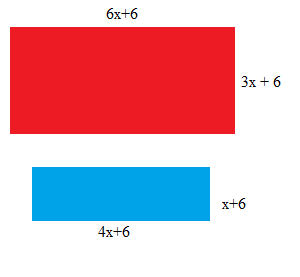
\includegraphics[width=2.04167in,height=1.8873in]{./imgSAEB_8_MAT/media/image5.png}
\end{figure}

\reduline{ Considerando que a fórmula da área de um retângulo é l \cdot l, temos que\hfill}\\
\reduline{ Terreno vermelho: $(6x + 6) \cdot (3x + 6)= 18x^2 + 18x + 18x + 36= 18x^2 + 36x + 36$\hfill}\\
\reduline{ Terreno azul: $(4x + 6) \cdot (x + 6) = 4x^2 + 24x + 6x + 36 = 4x^2 + 30x + 36 =...$\hfill}\\
\reduline{ Somando os dois terrenos, temos que $18x^2 + 36x + 36 + 4x^2 + 30x + 36 =...$\hfill}\\
\reduline{ Área total dos dois terrenos $= 22x^2 + 66x + 72$\hfill}\\

\num{10} Efetue os monômios descritos abaixo:


\begin{multicols}{2}
\begin{escolha}[itemsep=0pt,leftmargin=0pt]
\item $(6x^4+ 12x^6)$
    \rosa{$6x^4 + 12x^6 = 18x^{10}$}
\item $10xy-xy$
    \rosa{$10xy - xy = 9xy$}
\item $(6x^3) \cdot (2x^2)$
    \rosa{$(6x^3) \cdot (2x^2) = (12x^5)$}
\item $((14x^{10})): (2x^2)$
    \rosa{$((14x^10) \div (2x^2)=7x^8)$}
\item $(2x^3)^3$
    \rosa{$(2x^3)^3= (2x^9)$}
\item $(-4xy^2) ^3$
    \rosa{$(-4xy^2)^3= (-4xy^6)$}
\item $(\frac{30x}{6x})$, para $x$ diferente de $0$
    \rosa{$(\frac{30x}{6x}), para x diferente de 0 = 5x$}
\item $6x^2 - 8x^2$
    \rosa{$6x^2 - 8x^2 = -2x^2$}
\item $((\frac{4}{5}x)^{-1})$
    \rosa{$((\frac{4}{5}x)^{-1}) = (\frac{5}{4})$}
\item $9x^2 + 6x^2$
    \rosa{$ 9x^2 + 6x^2 = 15x^2$}
\item $7x^2 + 4x$
    \rosa{$7x^2 + 4x^2 = 11x^2$}
\item $(8r) \cdot (6s)$
    \rosa{$(8r) \cdot (6s) = 48rs$}
\item $(16x^2) \div 4$
    \rosa{$(16x^2) \div 4 = 4x^2$}
\item $8x + 6x + 4x$
    \rosa{$8x + 6x + 4x = 18x$}
\item $(-4xy^2)^3$
    \rosa{$((-2xy^2)^4)= (16x^4 y^8)$}
\end{escolha}
\end{multicols}

\pagebreak

\section{Treino}

\num{1} Elza resolveu comprar uma piscina com as medidas abaixo:

\begin{figure}[H]
\centering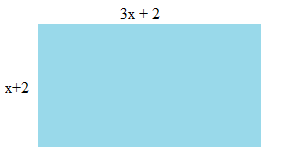
\includegraphics[width=2.9625in,height=1.67014in]{./imgSAEB_8_MAT/media/image6.png}
\end{figure}

Qual é a equação que representa a medida da área em $m^2$ dessa piscina?

\begin{escolha}[itemsep=0pt]
\item $3x^2 + 8x + 4$ \rosa{-- X}
\item $8x + 8$
\item $4x + 4$
\item $3x + 1$
\end{escolha}

% SAEB: Resolver problemas que envolvam cálculo do valor numérico de
% expressões algébricas.

% BNCC: EF08MA10 -- Identificar a regularidade de uma sequência numérica
% ou figural não recursiva e construir um algoritmo por meio de um
% fluxograma que permita indicar os números ou as figuras seguintes.

% A: Correta, pois, considerando a medida dos lados, temos que:

% 3x + 2 \cdot x + 2=

% (3x + 2) \cdot (x + 2)=

% Utilizando a distributiva:

% 3x^2 + 6x + 2x + 4

% 3x^2 + 8x + 4

% B: Incorreta, pois o aluno poderia confundir o enunciado e colocar o
% resultado do perímetro.

% C: Incorreta, pois o aluno poderia realizar uma soma ao invés de uma
% multiplicação.

% D: Incorreta, pois o aluno poderia chegar a esse valor realizando uma
% divisão ao invés de uma multiplicação.

\num{2} Considerando que $a^2+ b^2 = 34$ e $ab= 15$, qual é o valor de
$(\frac{(a + b)^2}{8})$?

\begin{escolha}[itemsep=0pt]
\item $2,266666666$
\item $19$
\item  $8$ \rosa{-- X}
\item $9,25$
\end{escolha}






% SAEB: Resolver problemas que envolvam cálculo do valor numérico de
%\begin{comment} %Jorge: Felipe, segue daqui pra cima!
% expressões algébricas.

% BNCC: EF08MA10 -- Identificar a regularidade de uma sequência numérica
% ou figural não recursiva e construir um algoritmo por meio de um
% fluxograma que permita indicar os números ou as figuras seguintes.

% A: Incorreta, pois o aluno chegaria a essa conclusão apenas dividindo um
% termo pelo outro.

% B: Incorreta, pois o aluno chegaria a essa conclusão realizando apenas a
% subtração de um termo pelo outro.

% C: Correta, pois

% (\frac{(a + b)^2}{8}\ ) = (\frac{a^{2} + 2ab + b^2}{8})

% Fazendo a substituição de a^2 + b^2 = 34 e ab = 15, temos que:

% (\frac{34 + (2.15)}{8} =) (\frac{34 + 30}{8}) = (\frac{64}{8}) = 8

% D: incorreta, pois foi realizada a soma ao invés da multiplicação no
% último termo.

\num{3} O diâmetro de um disco de vinil é igual a $(x^2 - 3)$. A partir desse
valor, quanto valem o perímetro e a área do disco?

Considere $(\pi) = 3$.

\begin{escolha}[itemsep=0pt]
\item $($Área $= 3x^4 - 18x^2 - 27$; Perímetro $= 6x^2 - 18)$
\item $($Área $= 3x^4 - 18x^2 + 27$; Perímetro $= 6x^2 + 18)$
\item $($Área $= 3x^4 + 18x^2 + 27$; Perímetro $= 6x^2 - 18)$
\item  $($Área $= 3x^4 - 18x^2 + 27$; Perímetro $= 6x^2 - 18)$ \rosa{-- X}
\end{escolha}




% SAEB: Resolver problemas que envolvam cálculo do valor numérico de
% expressões algébricas.

% BNCC: EF08MA10 -- Identificar a regularidade de uma sequência numérica
% ou figural não recursiva e construir um algoritmo por meio de um
% fluxograma que permita indicar os números ou as figuras seguintes.

% A: Incorreta, pois o aluno, ao errar o jogo de sinal no cálculo da área,
% encontrará esse valor.

% B: Incorreta, pois o aluno, ao errar o jogo de sinal no cálculo do
% perímetro, encontrará esse valor.

% C: Incorreta, pois o aluno, ao errar o jogo de sinal no cálculo da área,
% encontrará esse valor.

% D: Correta, pois, para o cálculo da área, temos:

% (A = \pi r^{2}).

% Logo,

% A = 3 \cdot (x^2-3) ^2

% A = 3 \cdot ((x^4) - 6x^2 + 9)

% A = (3x^4) - 18x^2 + 27

% Perímetro

% P= 2(\text{\ π\ .\ r})

% P = 2 \cdot 3. (x^2-3)

% P = 2 \cdot (3x^2 - 9)

% P = 6x^2 - 18


\chapter{Equações polinomiais de 2º grau}

\section{Habilidades do SAEB} 

% Inferir uma equação polinomial de 2º. grau que modela um problema.

\begin{itemize}
\item
  Resolver uma equação polinomial de 2º. grau.
\item
  Resolver problemas que possam ser representados por equações
  polinomiais de 2º grau.
\end{itemize}

\subsection{Habilidade da BNCC}

\begin{itemize}
 \item EF08MA09.
\end{itemize}

\conteudo{
\smallskip\noindent\textbf{Equação polinomial de 2º. grau}\quad
São consideradas equações polinomiais de 2º. grau aquelas encontradas na
forma $ax^2 + b = 0$.

Por exemplo:

Qual é a solução da equação $x^2 - 9 = 0$, no conjunto $R$?

Temos que:

$$x^2 - 9 = 0$$
$$x^2 = 9$$
$$x = (\sqrt{9})$$
$$x = \pm 3$$

O conjunto solução é $(-3, 3)$.

A resolução da equação $16x^2 - 1 = 0$ é

$$16x^2 = 1$$
$$x = (\pm \sqrt{\frac{1}{16}})$$
$$x = (\pm \frac{1}{4})$$

Logo, o conjunto solução é $(+ \frac{1}{4})$ e $(- \ \frac{1}{4})$}




\section{Atividades}

\num{1} Determine a solução da equação $x^2 + 4 = 0$ no conjunto R.

\reduline{ $x^2 + 4 = 0; x^2 = - 4; X= (\sqrt{- 4})$\hfill}\\

Como $(\sqrt{- 4})$ não existe no conjunto R, não temos valores reais
para x. Logo, a equação não tem raízes reais. Assim, $S = 0$.

\num{2} Resolva, no conjunto R, a equação $(2y + 1)^2 = 8 + 2(2y + 1)$.

\reduline{$ (2y + 1)(2y + 1) = 8 + 2(2y + 1); 4y^2 + 2y + 2y + 1 = 8 + 4y + 2; 4y^2 + 4y + 1 = 10 + 4y; $\hfill}\\
\reduline{$ 4y^2 + 4y - 4y + 1 - 10 = 0; 4y^2 - 9 = 0; Y = \pm (\sqrt{\frac{9}{4}}); Y= \pm (\frac{3}{2})$\hfill}  

Logo os números + $(\frac{3}{2}) e (\frac{3}{2})$ são as raízes da
equação.

\num{3} Determine o conjunto solução de cada uma das seguintes equações do
2°. grau, no conjunto R.


% Jorge: Autor não colocou a resposta.
\begin{escolha}[itemsep=0pt]
\item $x^2 - 1 = 0$
        \rosa{$( -1,1)$}
\item $x^2 - 16 = 0$
        \rosa{$( -4, 4)$}
\item $x^2 - 64 = 0$
        \rosa{$(-8, 8)$}
\item $9x^2 = 25$
        \rosa{$(\left(- \frac{5}{3}\right ) ,(\frac{5}{3}) )$}
\end{escolha}




\num{4} Identifique $a, b$ e $c$ nas funções quadráticas abaixo:



\begin{escolha}[itemsep=0pt]
\item $x^2 - 5x + 6 = 0$
        \rosa{$a = 1; b = -5; c = 6$;}
\item $-2x^2 + 8x - 8 = 0$
        \rosa{$a = -2; b = 8; c = -8$;}
\item $x^2 = 4$
        \rosa{$a = 1; b = 0; c = 4$;}
\item $x^2 - x = - (x + 15)$
        \rosa{$a = 1; b = 0; c = 15$}
\end{escolha}





\num{5} A idade do filho mais novo de Joana é representado pela equação $x^2 -
100 = 0$. Qual é a idade do filho mais novo de Joana?

\reduline{ Realizando a equação temos que:\hfill}\\
\reduline{ $x^2 - 100 = 0; x^2 = 100; x = (\sqrt{100}); x = \pm10$\hfill}\\
\reduline{Como a idade não pode ser representada, com números negativos, temos que\hfill}\\
\reduline{a idade do filho mais novo de Joana é 10 anos.\hfill}

\pagebreak

\num{6} Marcos é dono de uma madeireira que vende blocos de madeira de 2
tamanhos diferentes. Os tamanhos são definidos, em metros, pelas raízes
da equação $x^2 - 5x + 4 = 0$. Quais são os tamanhos de madeira disponíveis
na madeireira de marcos?

\reduline{Temos que: $x^2 - 5x + 4 = 0; A = 1; B = - 5; C = 4$\hfill}\\
\reduline{$(\frac{- ( - 5) \pm \sqrt{{- 5}^{2} - 4.\ 1.4}}{2.1})$;$(\frac{5 \pm \sqrt{25 - 16}}{2})$;\hfill}\\
\reduline{$(\frac{5 \pm \sqrt{9}}{2})$;$(\frac{5 \pm 3}{2})$\hfill}\\
\reduline{$(x_1) = (\frac{5 + 3}{2})= (\frac{8}{2}) = 4; (x_2) = (\frac{5 - 3}{2})= (\frac{2}{2})=1$\hfill}
\reduline{Logo, os tamanhos disponíveis de madeira são 1 metro e 4 metros.\hfill}

\num{7} Evandro é corredor. Certo dia, resolveu participar de uma maratona
com seu amigo José. Como Evandro é mais experiente, largou na frente e
abriu certa vantagem. A distância de Evandro e José em km é definida
pela equação $x^2 - 4x + 4 = 0$. Sendo assim, quantos km Evandro está na
frente de José?

\reduline{ $x^2 - 4x + 4 = 0; A = 1; B = -4; C = 4$\hfill}\\
\reduline{ $(\frac{- ( - 4) \pm \sqrt{{( - 4)}^{2} - 4\ .\ 1.\ 4}}{2\ .\ 1})$\hfill}\\
\reduline{ $(\frac{4 \pm \sqrt{16 - 16}}{2}); (\frac{4}{2}) = 2 km$\hfill}\\

\num{8} Raiane vai para o trabalho todos os dias a pé. A distância de sua
casa para o seu tralho em km é a soma das raízes da equação $2x^2 − 6x − 8
= 0$. Quantos km Raiane anda por dia para ir ao trabalho?

\reduline{ $2x^2 − 6x − 8 = 0; A = 2; B = -6; C = -8$\hfill}\\
\reduline{ $(\frac{- ( - 6) \pm \sqrt{{( - 6)}^{2} - 4.2.( - 8)}}{2.2})$\hfill}\\
\reduline{ $(\frac{6 \pm \sqrt{36 + 64}}{4}); (\frac{6 \pm \sqrt{100}}{4}); (\frac{6 \pm 10}{4})$\hfill}\\
\reduline{ $X1= (\frac{6 + 10}{4}) = (\frac{16}{4}) = 4; X2= (\frac{6 - 10}{4}) = (\frac{- 4}{4}) = -1$\hfill}\\
\reduline{ Somando ambas as raízes, temos que Raiane anda 3km por dia para ir ao trabalho.\hfill}\\

\pagebreak

\num{9} Divina tem 2 filhas com idades diferentes, representadas pelas raízes
da equação $x^2 - 20x + 36 = 0$. Quais são as idades das filhas de Divina?

\reduline{ $x^2 - 20x + 36 = 0$\hfill}\\
\reduline{ $A= 1; B= -20; C= 36$\hfill}\\
\reduline{ $(\frac{- ( - 20) \pm \sqrt{{( - 20)}^{2} - 4.1.36}}{2.1})$\hfill}\\
\reduline{ $(\frac{20 \pm \sqrt{400 - 4.1.36}}{2a})$\hfill}\\
\reduline{ $(\frac{20 \pm \sqrt{400 - 144}}{2})$\hfill}\\
\reduline{ $(\frac{20 \pm \sqrt{256}}{2})$\hfill}\\
\reduline{ $(\frac{20 \pm 16}{2}); X1 = (\frac{20 + 16}{2})= (\frac{36}{2} =) 18; X2 = (\frac{20 - 16}{2}) = (\frac{4}{2}) = 2$\hfill}\\
\reduline{ Logo, as filhas de Divina têm 18 anos e 2 anos.\hfill}\\

\num{10} Mateus pretende pagar uma dívida com o banco. Ele sabe que o valor que o
valor que deve é a soma das raízes da equação $x^2 + 4x + 3 = 0$ multiplicada
por 1.000. Sendo assim, quantos reais Mateus deve ao banco?


\reduline{B: Correta, pois, utilizando Bhaskhara, temos: $x^2 - 7x = 0$; $A = 1$; $B = - 7$; $C = 0$;\hfill}\\
\reduline{$(\frac{- ( - 7) \pm \sqrt{{( - 7)}^{2} - 4.1.0}}{2.1})$;\hfill}\\
\reduline{$(\frac{7 \pm \sqrt{49}}{2})$; $(\frac{7 \pm 7}{2})$;\hfill}\\
\reduline{$x_1 = (\frac{7 + 7}{2})\$ = (\frac{14}{2}) = 7$; $x_2 = (\frac{7 - 7}{2}) = 0$\hfill}\\
\linhas{3}

% Logo, realizando a soma de 7 + 0 = 7, obtemos que Clebinho chutou 7
% vezes ao gol.
% 
% C: Incorreta, pois o aluno pode chegar a essa conclusão considerando que
% o enunciado pede apenas o valor antes de extrairmos as raízes da
% equação.
% 
% D: Incorreta, pois o aluno pode chegar a essa conclusão esquecendo de
% dividir o valor de uma das raízes por 2.

% \num{2} Daniel é piloto de corridas de alta velocidade. Em uma certa prova,
% ele ficou em 2° lugar. A distância em segundos do primeiro colocado para
% Daniel é a soma das raízes da equação $4x^2 + 9x = 0.$ Quanto tempo depois
% do primeiro colocado Daniel Chegou?

% \begin{enumerate}
% \item 0
% \item 81
% \item 9
% \item 2,25
% % \end{enumerate}

% SAEB: Resolver problemas que possam ser representados por equações
% polinomiais de 2º grau.

% BNCC: EF08MA09 -- Resolver e elaborar, com e sem uso de tecnologias,
% problemas que possam ser representados por equações polinomiais de 2º
% grau do tipo ax2 = b.
% que deve é a soma das raízes da equação $x^2 + 4x + 3 = 0~\text{multiplicada}$ por
% 1.000. Sendo assim, quantos reais Mateus deve ao banco?

\reduline{ Utilizando Bhaskhara, temos: $x^2 + 4x + 3 = 0; A = 1; B = 4; C = 3\hfill$}\\
\reduline{ $(\frac{- 4 \pm \sqrt{4^{2} - 4.1.3}}{2.1}$)\hfill}\\
\reduline{ $(\frac{- 4 \pm \sqrt{16 - 4.1.3}}{2.1}); (\frac{- 4 \pm \sqrt{4}}{2})$\hfill}\\
\reduline{ $X1= (\frac{- 4 + 4}{2}) = 0; X2 = (\frac{- 4 - 4}{2}) = -4$\hfill}\\
\reduline{ Multiplicando por 1.000, temos que $-4 \cdot 1000 = - 4000$. Logo, Mateus deve R\$\,4.000,00 ao banco.\hfill}\\

\pagebreak
\section{Treino}

\num{1} Clebinho é atacante de um famoso time de futebol. Durante uma
partida, o número de suas finalizações ao gol foi a soma das raízes da
equação $x^2- 7x = 0.$ Quantas vezes Clebinho chutou no gol durante a
partida?

\begin{escolha}[itemsep=0pt]
\item 0
\item 7
\item 49
\item 14
\end{escolha}

% SAEB: Resolver problemas que possam ser representados por equações
% polinomiais de 2º grau.

% BNCC: EF08MA09 -- Resolver e elaborar, com e sem uso de tecnologias,
% problemas que possam ser representados por equações polinomiais de 2º
% grau do tipo ax2 = b.

% A: Incorreta, pois o aluno pode chegar a essa conclusão considerando que
% o enunciado pede apenas 1 valor das raízes da equação.


% A: Incorreta, pois o aluno pode chegar a essa conclusão considerando que


% %% Encontro Felipe Jorge

% A: Incorreta, pois o aluno pode chegar a essa conclusão considerando que
% o enunciado pede apenas 1 valor das raízes da equação.

% B: Correta, pois, utilizando Bhaskhara, temos:

% x^2 - 7x = 0

% A = 1

% B = - 7

% C = 0

% (\frac{- ( - 7) \pm \sqrt{{( - 7)}^{2} - 4.1.0}}{2.1})

% (\frac{7 \pm \sqrt{49}}{2})

% (\frac{7 \pm 7}{2})

% X1 = (\frac{7 + 7}{2})\$ = (\frac{14}{2}) = 7

% X2 = (\frac{7 - 7}{2}) = 0

% Logo, realizando a soma de 7 + 0 = 7, obtemos que Clebinho chutou 7
% vezes ao gol.

% C: Incorreta, pois o aluno pode chegar a essa conclusão considerando que
% o enunciado pede apenas o valor antes de extrairmos as raízes da
% equação.

% D: Incorreta, pois o aluno pode chegar a essa conclusão esquecendo de
% dividir o valor de uma das raízes por 2.

\num{2} Daniel é piloto de corridas de alta velocidade. Em uma certa prova,
ele ficou em 2° lugar. A distância em segundos do primeiro colocado para
Daniel é a soma das raízes da equação $4x^2 + 9x = 0$. Quanto tempo depois
do primeiro colocado Daniel Chegou?

\begin{escolha}[itemsep=0pt]
\item 0
\item 81
\item 9
\item 2,25
\end{escolha}

% SAEB: Resolver problemas que possam ser representados por equações
% polinomiais de 2º grau.

% BNCC: EF08MA09 -- Resolver e elaborar, com e sem uso de tecnologias,
% problemas que possam ser representados por equações polinomiais de 2º
% grau do tipo ax2 = b.

% A: Incorreta, pois o aluno pode chegar a essa conclusão considerando que
% o enunciado pede apenas 1 valor das raízes da equação descrita.

% B: Incorreta, pois o aluno pode chegar a essa conclusão considerando que
% o enunciado pede apenas o valor antes de extrairmos as raízes da equação
% descrita.

% C: Incorreta, pois o aluno pode chegar a essa conclusão esquecendo de
% dividir o valor de uma das raízes por 4.

% D: Correta, pois, utilizando Bhaskhara, temos:

% 4x^2 + 9x = 0

% A = 4

% B = 9

% C = 0

% (\frac{- 9 \pm \sqrt{9^{2} - 4.4.0}}{2.4})

% (\frac{- 9 \pm \sqrt{81}}{8})

% (\frac{- 9 \pm 9}{8})

% X1 = (\frac{- 9 + 9}{8}) = 0

% X2= (\frac{- 9 - 9}{8}) = (\frac{- 18}{8}) = - (\frac{9}{4}) =
% -2,25 segundos

\num{3} Antônio foi ao posto de gasolina abastecer seu carro. Ele descobriu
que a quantidade do tanque que foi preenchida por gasolina é igual à
soma das raízes da equação $6x^2 - 5x = 0$. Qual foi esta parte preenchida?

\begin{escolha}[itemsep=0pt]
\item 25
\item 0
\item $(\frac{5}{6})$
\item 11
\end{escolha}

% SAEB: Resolver problemas que possam ser representados por equações
% polinomiais de 2º grau.

% BNCC: EF08MA09 -- Resolver e elaborar, com e sem uso de tecnologias,
% problemas que possam ser representados por equações polinomiais de 2º
% grau do tipo ax2 = b.

% A: Incorreta, pois o aluno pode chegar a esse valor ao não realizar a
% radiciação necessária.

% B: Incorreta, pois o aluno pode chegar a essa conclusão considerando que
% o enunciado pede apenas 1 valor das raízes da equação descrita.

% C: Correta, pois, utilizando Bhaskhara, temos:

% 6x^2 - 5x = 0

% A = 6

% B = -5

% C = 0

% (\frac{- ( - 5) \pm \sqrt{{( - 5)}^{2} - 4.6.0}}{2( - 5)})

% (\frac{5 \pm \sqrt{25}}{12})

% (\frac{5 \pm 5}{12})

% X1 = (\frac{5 + 5}{12}) = (\frac{10}{12}) = (\frac{5}{6})

% X2 = (\frac{5 - 5}{12}) = 0

% Logo, temos que a parte preenchida do tanque foi de (\frac{5}{6}).

% D: Incorreta, pois o aluno chegaria a esse valor apenas somando os
% termos da equação e não realizando a operação por completo.


\chapter{Proporções}

\subsection{Habilidade SAEB}

\begin{itemize}
\item Resolver problemas que envolvam variação de
proporcionalidade direta ou inversa entre duas ou mais grandezas,
inclusive escalas, divisões proporcionais e taxa de variação.
\end{itemize}

\subsection{Habilidades da BNCC}

\begin{itemize}
\item EF08MA12, EF08MA13.
\end{itemize}

\conteudo{Sendo a e b dois números racionais, sendo b maior que 0, denomina-se razão entre a
e b ou razão de a para b o quociente a/b. Essa razão
pode ser lida de uma das seguintes maneiras:
razão de a para b ou ``a está para b''.

Uma das aplicações da ideia de razão entre duas grandezas encontra-se na
escala de redução e na escala de ampliação, conhecidas simplesmente como
escala.

Denomina-se escala de um desenho a razão entre o comprimento considerado
nele e o correspondente comprimento real, medidos com a mesma unidade.
Em geral, utilizamos as medidas em centímetros para determinar uma
escala.

Outra razão comum é a densidade de um corpo. 
Para calculá-la, aplicamos a ideia de razão
entre duas grandezas. Assim, a densidade de um corpo é dada pela razão
entre a massa e o volume desse corpo.}



\section{Atividades}




\num{1} Um prêmio de loteria, no valor de R\$\,2.700.000,00 será dividido
igualmente pelo total de acertadores.

\begin{escolha}[itemsep=0pt]
\item Quanto cada acertador receberá, caso o prêmio seja dividido entre 3 ganhadores?
\item E se fossem 8 ganhadores?
\item Conforme o número de acertadores aumenta, o que acontece com o valor do prêmio?
\end{escolha}

\reduline{Ao dividirmos o valor do prêmio proporcionalmente, entre 3 ganhadores\hfill}\\
 \reduline{temos que $2.700.000 \div 3 = 900.000$ para cada um.\hfill}\\
\reduline{Ao dividirmos o valor do prêmio proporcionalmente entre 8 ganhadores\hfill}\\
\reduline{temos que $2.700.000 \div 8 = 337.500$ para cada um.\hfill}\\
\reduline{Quando o número de acertadores aumenta, o valor do prêmio diminui.\hfill}\\



\num{2} A distância entre a Terra e o Sol é de, aproximadamente, $150.000.000 km$; 
A luz do Sol, para atingir a Terra, leva em torno de 500 segundos.

\begin{escolha}[itemsep=0pt]
\item Qual é a velocidade da luz no vácuo?
\item Quantos minutos a luz do Sol leva para chegar à Terra?
\end{escolha}

    \reduline{ Utilizando a razão $(\frac{distância}{\text{tempo}})$, temos que $(\frac{150\ 000\ 000}{500}) = 300 000 km/s$\hfill}\\
    \reduline{ se $60$ segundos = $1$ minuto, temos que $500 \div 60 = 8$ minutos e $20$ segundos.\hfill}\\






\num{3} Um novo condomínio de casas está sendo construído, e sua planta foi
representada, em uma folha de papel, com $5,5$ cm de comprimento por $3,125$
cm de largura. Sabendo que a escala utilizada foi $1 \div 16 000$, determine
as dimensões reais deste condomínio.

\reduline{ Como a escala é de $1 \div 16.000$, temos que:\hfill}\\
\reduline{ Comprimento $5,5 \cdot 16.000 = 88.000 cm$\hfill}\\
\reduline{ Largura $3,125 \cdot 16.000 = 50.000 cm$\hfill}\\
\reduline{ Comprimento $= 880 m$; largura $= 500 m$\hfill}\\

\num{4} Um bloco maciço de madeira tem $54 kg$ de massa e ocupa um volume de $3
m^3$. Qual é a densidade desse bloco?

\reduline{ $d = \frac{54}{3}$\hfill}\\
\reduline{ $d = 18 kg/m^3$\hfill}\\

\num{5} Um fio de cobre utilizado na fiação de uma casa comum ocupa um volume
de $0,2 cm^3$. Sabendo que a massa do fio é de $4,3 g$, determine a densidade
desse metal.

\reduline{ $d = \frac{4,3}{0,2}$\hfill}\\
\reduline{ $d = 21,5 g/cm^3$\hfill}\\

\pagebreak

\num{6} Um país situado no continente europeu tem cerca de $135.000 km^2$ de
área e uma população de $12.200.000$ habitantes. Qual é a densidade
demográfica aproximada desse país?

\reduline{ Utilizando a razão da densidade demográfica (d), temos:\hfill}\\
\reduline{ $d = \frac{número de pessoas}{dimensão do espaço em km^2}$\hfill}\\
\reduline{ $d = \frac{12.200.000}{135.000}$\hfill}\\
\reduline{ $d = 90,37 habitantes/km^2$\hfill}\\

\num{7} Cinco homens levam 20 dias para recapear um trecho de estrada. Esse
mesmo serviço seria realizado em quantos dias, se fossem 8 homens no
total?

\reduline{ Utilizando a Regra de 3 simples. temos que:\hfill}\\
\reduline{ $(\frac{5}{8} = \frac{20}{x}$)\hfill}\\
\reduline{ $5 \cdot 20 = 8 \cdot x$\hfill}\\
\reduline{ $100 = 8x$\hfill}\\
\reduline{ $x= 12,5$\hfill}\\

\num{8} Uma padaria produz $260$ pães franceses a cada $50$ min. Em uma jornada
de $12 h$, quantos pães são produzidos?

\reduline{ Utilizando a Regra de 3 simples, temos que:\hfill}\\
\reduline{ $(\frac{260}{x} = \frac{50}{720})$\hfill}\\
\reduline{ $187 200 = x$ \cdot 50\hfill}\\
\reduline{ $x = 3744$ pães são produzidos\hfill}\\

\num{9} Um livro tem $180$ páginas, e cada página tem $46$ linhas. Um editor
resolveu colocar apenas $30$ linhas em cada página. Qual será a nova
quantidade de páginas do livro?

\reduline{ Utilizando a regra de $3$ simples, temos que:\hfill}\\
\reduline{ ($\frac{180}{x} = \frac{46}{30})$\hfill}\\
\reduline{ $180 \cdot 46 = 30 \cdot x$\hfill}\\
\reduline{ $8280 = 30x$\hfill}\\
\reduline{ $x = 276$\hfill}\\

\num{10} Converta as velocidades dadas em m/s para km/h.

\begin{multicols}{3}
\begin{enumerate}[itemsep=-3pt]
\item $20 m/s$
        \rosa{$20 m/s \cdot 3,6 = 72 km/h$}
\item $100 m/s$
        \rosa{$100 m/s \cdot 3,6 = 360km/h$}
\item $55 m/s$
        \rosa{$55 m/s \cdot 3,6 = 198 km/h$}
\item $67 m/s$
        \rosa{$67 m/s \cdot 3,6 = 241,2 km/$h}
\item $90 m/s$
        \rosa{$90 m /s \cdot 3,6 = 324 km/h$}
\item $25 m/s$
        \rosa{$25 m/s \cdot 3,6 = 90 km/h$}
\item $30 m/s$
        \rosa{$30 m/s .3,6 = 108 km/h$}
\item $40 m/s$
        \rosa{$40 m/s \cdot 3,6 = 144km/h$}
\end{enumerate}
\end{multicols}


\section{Treino}

\num{1} Dona Estela está preparando a ceia de Natal para sua família e
comprou um peru de $4,2 kg$ para servir. Ao pesquisar sobre o tempo de
cozimento de um peru, descobriu que o tempo depende de sua massa em
quilogramas. Sabendo que um peru de $3,5 kg$ leva $2h15min$ para assar,
quanto tempo o prato que Dona estela comprou deve ficar no forno?

\begin{escolha}%[itemsep=-3pt][itemsep=0pt]
\item 2 horas e 42 minutos
\item 1 Horas e 52 minutos
\item 2 horas e 58 minutos
\item 567 minutos
\end{escolha}

% SAEB: Resolver problemas que envolvam variação de proporcionalidade
% direta ou inversa entre duas ou mais grandezas, inclusive escalas,
% divisões proporcionais e taxa de variação.

% BNCC: EF08MA13 -- Resolver e elaborar problemas que envolvam grandezas
% diretamente ou inversamente proporcionais, por meio de estratégias
% variadas.

% A: Correta, pois, utilizando a regra de 3 simples, temos que:

% (\frac{3,5}{4,2} = \frac{135}{x})

% 3,5 \cdot x = 567

% x = 162 minutos ou 2 horas e 42 minutos.

% B: Incorreta, o aluno poderia chegar a esse valor realizando a
% multiplicação reta na regra de 3 e não a multiplicação cruzada.

% C: Incorreta, pois esse seria o valor caso o aluno não convertesse horas
% em minutos como forma de solução.

% D: Incorreta, pois o aluno chegaria a esse resultado caso não realizasse
% a última operação necessária, que é a divisão.

\num{2} 5 rosquinhas de coco possuem 64 calorias. Dirce consome diariamente 3
unidades desse doce em seu café da manhã. Quantas calorias procedentes
das rosquinhas Dirce consome por dia?

\begin{escolha}[itemsep=0pt]
\item 106,6 calorias
\item 38,4 calorias
\item 960 calorias
\item 192 calorias
\end{escolha}

% SAEB: Resolver problemas que envolvam variação de proporcionalidade
% direta ou inversa entre duas ou mais grandezas, inclusive escalas,
% divisões proporcionais e taxa de variação.

% BNCC: EF08MA13 -- Resolver e elaborar problemas que envolvam grandezas
% diretamente ou inversamente proporcionais, por meio de estratégias
% variadas.

% A: Incorreta, pois o aluno chegaria nesse resultado multiplicando reto a
% regra de três ao invés de multiplicar cruzado.

% B: Correta, pois, utilizando a Regra de 3 simples, temos que:

% (\frac{5}{3} = \frac{64}{x})

% 5x = 64 \cdot 3

% 5x = 192

% x = 38,4

% C: Incorreta, pois o aluno chegaria a esse valor caso, no final da
% expressão, ao invés de realizar uma divisão, realizasse uma
% multiplicação.

% D: Incorreta, pois o aluno chegaria a essa conclusão considerando cada
% rosquinha com 64 calorias.

\num{3} Leandro tem um cachorro da raça fila brasileiro que pesa 27 kg. Para
tratar uma infecção nas vias urinárias, o veterinário receitou um
antibiótico cuja dosagem é de 9 ml a cada 10 kg de peso corporal.
Quantos ml de antibiótico Leandro dará a seu cachorro?

\begin{escolha}[itemsep=0pt]
\item $3,3333\ldots mL$
\item $24,3 mL$
\item $2430 mL$
\item $2,43 mL$
\end{escolha}

% SAEB: Resolver problemas que envolvam variação de proporcionalidade
% direta ou inversa entre duas ou mais grandezas, inclusive escalas,
% divisões proporcionais e taxa de variação.

% BNCC: EF08MA13 -- Resolver e elaborar problemas que envolvam grandezas
% diretamente ou inversamente proporcionais, por meio de estratégias
% variadas.

% A: Incorreta, pois o aluno chegaria a esse resultado realizando uma
% multiplicação reta ao invés de uma multiplicação cruzada.

% B: Correta, pois, utilizando a regra de 3 simples, temos que:

% (\frac{10}{27} = \frac{9}{x})

% 10.x = 9 \cdot 27

% 10x = 243

% x = 24,3 ml

% C: Incorreta, pois o aluno chegaria a essa conclusão se, ao final da
% expressão, realizasse uma multiplicação.

% D: Incorreta, pois o aluno chegaria a essa conclusão deslocando a
% virgula uma casa para esquerda durante o cálculo final.


\chapter{Polígonos}

\section{Habilidades do SAEB}

\begin{itemize}
\item Identificar, no plano cartesiano, figuras obtidas
por uma ou mais transformações geométricas (reflexão, translação,
rotação).
\item
  Relacionar o número de vértices, faces ou arestas de prismas ou
  pirâmides, em função do seu polígono da base.
\item
  Relacionar objetos tridimensionais às suas planificações ou vistas.
\item
  Classificar polígonos em regulares e não regulares. Reconhecer
  polígonos semelhantes ou as relações existentes entre ângulos e lados
  correspondentes nesses tipos de polígonos.
\item
  Reconhecer circunferência/círculo como lugares geométricos, seus
  elementos (centro, raio, diâmetro, corda, arco, ângulo central, ângulo
  inscrito).
\item
  Construir/desenhar figuras geométricas planas ou espaciais que
  satisfaçam condições dadas.
\end{itemize}

\subsection{Habilidade da BNCC}

\begin{itemize}
\item EF08MA18.
\end{itemize}


\conteudo{Um polígono é uma figura geométrica plana formada por segmentos de reta
que se conectam, chamados de lados. Esses lados não se cruzam, exceto em
seus pontos finais. Cada ponto de encontro entre dois lados é chamado de
vértice.

Podemos Classificar os polígonos em convexos e não convexos.

Podemos destacar os seguintes elementos de um polígono: vértices, lados,
ângulos internos e externos e diagonais.

Utilizando a Fórmula $(d = \ \frac{n(n - 3)}{2})$ podemos determinar o
número de diagonais de um polígono

Utilizando a fórmula $(S = (n - 2) \cdot 180°)$, podemos calcular a
soma dos ângulos internos de um polígono.}

\section{Atividades}



% \num{1} Complete a Tabela com o nome dos polígonos segundo o número de lados.

% %Paulo, inserir uma tabela com as informações abaixo:

% \begin{longtable}[]{@{}ll@{}}
% \toprule
% Número de lados & Nome do polígono\tabularnewline
% \midrule
% \endhead
% 3 & Triângulo\tabularnewline
% 4 & ~\tabularnewline
% 5 & ~\tabularnewline
% 6 & ~\tabularnewline
% 7 & ~\tabularnewline
% 8 & ~\tabularnewline
% 9 & ~\tabularnewline
% 10 & ~\tabularnewline
% 11 & ~\tabularnewline
% 12 & ~\tabularnewline
% 15 & ~\tabularnewline
% 20 & ~\tabularnewline
% \bottomrule
% \end{longtable}

% R: \begin{longtable}[]{@{}ll@{}}
% \toprule
% Número de lados & Nome do Polígono\tabularnewline
% \midrule
% \endhead
% 3 & Triângulo\tabularnewline
% 4 & Quadrilátero\tabularnewline
% 5 & Pentágono\tabularnewline
% 6 & Hexágono\tabularnewline
% 7 & Heptágono\tabularnewline
% 8 & Octógono\tabularnewline
% 9 & Eneágono\tabularnewline
% 10 & Decágono\tabularnewline
% 11 & Eneágono\tabularnewline
% 12 & Dodecágono\tabularnewline
% 15 & Pentadecágono\tabularnewline
% 20 & Icoságono\tabularnewline
% \bottomrule
% \end{longtable}

\pagebreak

\num{1} Determine quais das figuras a seguir são polígonos.

\begin{figure}[H]
\centering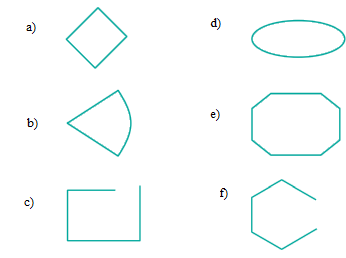
\includegraphics[width=1.7in,height=1.26763in]{./imgSAEB_8_MAT/media/image7.png}
\end{figure}
\reduline{ Somente as alternativas $A$ e $E$.\hfill}\\

\num{3} Classifique os polígonos a seguir em convexos e não convexos.

\begin{figure}[H]
\centering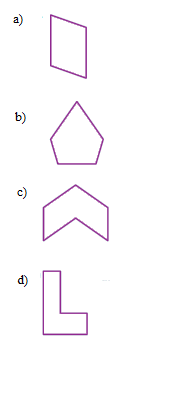
\includegraphics[width=1.16236in,height=2.36667in]{./imgSAEB_8_MAT/media/image8.png}
\end{figure}

\reduline{ a) Convexo.\hfill}\\
\reduline{ b) Convexo.\hfill}\\
\reduline{ c) Não convexo.\hfill}\\
\reduline{ d) Não convexo.\hfill}\\

\num{2} Utilizando a fórmula $d = \frac{n(n - 3)}{2}$, calcule o número
de diagonais de um polígono de

\begin{escolha}[itemsep=0pt]
\item 5 lados.
        \rosa{ $d = \frac{5(5 - 3)}{2} = (\frac{25 - 15}{2}) \frac{10}{2} = 5~\text{diagonais}$}
\item 9 lados.
        \rosa{ $d = \frac{9(9 - 3)}{2} = (\frac{81 - 27}{2} \frac{54}{2}) = 27~\text{diagonais}$}
\item 10 lados.
        \rosa{ $d = \frac{10(10 - 3)}{2} = \frac{100 - 30}{2} \frac{70}{2} = 35~\text{diagonais}$}
\item 15 lados.
        \rosa{ $d = \frac{15(15 - 3)}{2} = (\frac{225 - 45}{2}) \frac{180}{2}) = 90~\text{diagonais}$}
\item 20 lados.
        \rosa{ $d = \frac{20(20 - 3)}{2} = \frac{400 - 60}{2} \frac{340}{2} = 170~\text{diagonais}$}
\end{escolha}

\num{3} Utilizando a fórmula $Si = (n - 2) \cdot 180°$, calcule a soma dos ângulos
internos dos polígonos abaixo.

\begin{escolha}[itemsep=0pt]
\item Quadrilátero.
        \rosa{$Si = (4-2) \cdot 180°$;$Si = 2 \cdot 180°$; $Si = 360$}
\item Pentágono.
        \rosa{$Si = (5-2) \cdot 180°$;$Si = 3 \cdot 180$; $Si = 540$}
\item Eneágono.
        \rosa{$Si = (9-2) \cdot 180°$;$Si = 7 \cdot 180°$; $Si = 1260$}
\item Icoságono.
        \rosa{$Si = (20-2) \cdot 180°$;$Si = 18 \cdot 180°$; $Si = 3240$}
\item Dodecágono.
        \rosa{$Si = (12-2) \cdot 180°$;$Si = 10 \cdot 180$; $Si = 1800$}
\end{escolha}

\num{4} Utilizando a fórmula $Si = (n-2) \cdot 180°$, calcule o número de lados dos
polígonos cuja soma dos ângulos internos é:

\begin{escolha}[itemsep=0pt]
\item $1080°$
    \rosa{$1080 = (n-2) \cdot 180°; (\frac{1080}{180})= n - 2; 6 = n - 2; n = 8$}
\item $1980°$
    \rosa{$1980 = (n-2) \cdot 180°; (\frac{1980}{180}) = n - 2; 11 = n - 2; n = 13$}
\item $2340°$
    \rosa{$2340 = (n-2) \cdot 180°; (\frac{2340}{180}) = n - 2; 13 = n - 2; n = 15$}
\item $1800°$
    \rosa{$1800 = (n-2) \cdot 180°; (\frac{1800}{180}) = n - 2; 10 = n - 2; n = 12$}
\end{escolha}



\num{5} Considere o paralelogramo a seguir. Nele, estão expressas as medidas
de dois ângulos opostos. Quais são as medidas dos quatro ângulos desse
paralelogramo?

\begin{figure}[H]
\centering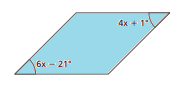
\includegraphics[width=1.82292in,height=0.95833in]{./imgSAEB_8_MAT/media/image9.png}
\end{figure}

\reduline{ $4x + 1 = 6x - 21$\hfill}\\
\reduline{ $-2x = -22$\hfill}\\
\reduline{ $x = 11$\hfill}\\
\reduline{ Substituindo $x = 11$ nas duas equações, temos que:\hfill}\\
\reduline{ $4 \cdot 11 + 1 = 45°$ e \hfill}\\
\reduline{ $6 \cdot 11 - 21 = 45°$.\hfill}\\
\reduline{ Como a soma dos ângulos internos de um paralelogramo é $360°$,\hfill}\\
\reduline{ $45° + 45° - 360° = 270°$ e \hfill}\\
\reduline{ $270° \div 2 = 135°$.\hfill}\\
\reduline{ Temos então que o paralelogramo possui $2$ ângulos de $45°$ e $2$ ângulos de $135°$.\hfill}

\pagebreak

\num{6} Calcule o valor de x e y na figura indicada.

\begin{figure}[H]
\centering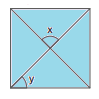
\includegraphics[width=1.03125in,height=1.03125in]{./imgSAEB_8_MAT/media/image10.png}
\end{figure}

\reduline{ Relembrando que a soma dos ângulos internos de um triangulo é $= 180°$ e\hfill}\\
\reduline{ que a soma dos ângulos internos de um paralelogramo é igual a $360°$,\hfill}\\
\reduline{ temos que $y=45°$ e $x = 90°$.\hfill}
\linhas{3}

\num{7} Determine a medida x no paralelogramo da figura a seguir.

\begin{figure}[H]
\centering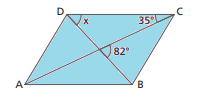
\includegraphics[width=2.05208in,height=1.09375in]{./imgSAEB_8_MAT/media/image11.png}
\end{figure}

\reduline{ Por método de observação, temos que o ângulo no ponto $B$ é:\hfill}\\
\reduline{ $82°+ 35° - 180° = 63°$\hfill}\\
\reduline{ Formando um triangulo $BCD$, temos que\hfill}\\
\reduline{ $70° + 63° - 180° = 47°$\hfill}
\linhas{3}

\pagebreak

\num{8} Analise a circunferência de centro A representada a seguir e
classifique em raio, diâmetro ou corda o segmento de reta:

\begin{figure}[H]
\centering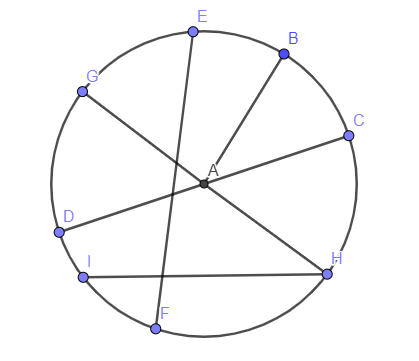
\includegraphics[width=2.98681in,height=2.57292in]{./imgSAEB_8_MAT/media/image12.png}
\end{figure}

\begin{enumerate}
\item GA

        \rosa{raio}
\item DC

        \rosa{diâmetro; corda}
\item EF

        \rosa{corda}
\item GH

        \rosa{diâmetro; corda}
\item AB

        \rosa{raio}
\item DA

        \rosa{raio}
\item HI

        \rosa{corda}
\item AC

        \rosa{raio}
\item AH

        \rosa{raio}
\end{enumerate}

\pagebreak

\section{Treino}

\num{1} Alfredo desenhou, em uma madeira, um eneágono regular cujo perímetro
era de $117 cm$. Qual é a medida de cada lado dessa figura?


\begin{escolha}
\item $13 cm$ 
\item $11,7 cm$
\item $16,71 cm$
\item $23,4 cm$
\end{escolha}

% SAEB: Construir/desenhar figuras geométricas planas ou espaciais que
% satisfaçam condições dadas.

% BNCC: EF08MA18 -- Reconhecer e construir figuras obtidas por composições
% de transformações geométricas (translação, reflexão e rotação), com o
% uso de instrumentos de desenho ou de softwares de geometria dinâmica.

% A: Correta, pois 117 \div 9 = 13 cm de lado tem essa figura.

% B: Incorreta, pois o aluno poderia chegar a essa conclusão caso
% considerasse que o eneágono regular possui 10 lados e não 9.

% c: Incorreta, pois o aluno poderia chegar a essa conclusão caso
% considerasse que o eneágono regular possui 7 lados e não 9.

% D: Incorreta, pois o aluno poderia chegar a essa conclusão caso
% considerasse que o eneágono regular possui 5 lados e não 9.

\num{2} O~centro do campo~de futebol é marcado com um ponto. Ao redor,
traçamos um~círculo~com raio de $9,15$ metros. Com essas informações em
mente, qual é a área do círculo central de um campo de futebol,
aproximadamente?

Considere $(\pi = 3)$:

\begin{escolha}
\item $54,1 m^2$
\item $27,41 m^2$
\item $251 m^2$ 
\item $27,66 m^2$
\end{escolha}

% SAEB: Construir/desenhar figuras geométricas planas ou espaciais que
% satisfaçam condições dadas.

% BNCC: EF08MA18 -- Reconhecer e construir figuras obtidas por composições
% de transformações geométricas (translação, reflexão e rotação), com o
% uso de instrumentos de desenho ou de softwares de geometria dinâmica.

% A: Incorreta, poiso aluno chegaria a esse valor caso confundisse a
% fórmula da área do círculo com a fórmula do perímetro do círculo.

% B: Incorreta, pois o aluno chegaria a essa conclusão caso se esquecesse
% do termo quadrático da expressão.

% C: Correta, pois

% (A = \pi r^{2})

% A = 3 \cdot 9,15^2

% A= 3. 83,7225

% A= 251 m^2

% D: Incorreta, pois o aluno chegaria a esse resultado caso dividisse a
% expressão no final da fórmula ao invés de multiplicar.

\num{3} Iolanda faz peças com tecidos. Uma das peças mais vendidas é um porta
joias com formato de um hexágono regular de $5 cm$ de lado com a borda
revestida com uma fita. Quantos centímetros de fita, no mínimo, Iolanda
precisa para confeccionar $20$ porta joias?

\begin{escolha}
\item $6 metros$ 
\item $600 metros$
\item $5 metros$
\item $4 metros$
\end{escolha}

% SAEB: Construir/desenhar figuras geométricas planas ou espaciais que
% satisfaçam condições dadas.

% BNCC: EF08MA18 -- Reconhecer e construir figuras obtidas por composições
% de transformações geométricas (translação, reflexão e rotação), com o
% uso de instrumentos de desenho ou de softwares de geometria dinâmica.

% A: Correta, pois:

% Hexágono regular = 6 lados

% 30 cm por porta joias

% 20 \cdot 30 cm = 600 cm de fita ou 6 metros de fita

% B: Incorreta, pois o aluno pode chegar a esse valor confundindo cm com
% metros.

% C: Incorreta, pois o aluno pode chegar a esse valor considerando que um
% hexágono regular contenha 5 lados.

% D: Incorreta, pois o aluno pode chegar a esse valor considerando que um
% hexágono regular contenha 4 lados.


\chapter{Triângulos}

\section{Habilidades do SAEB}

\begin{itemize}
\item Identificar propriedades e relações existentes
entre os elementos de um triângulo (condição de existência, relações de
ordem entre as medidas dos lados e as medidas dos ângulos internos, soma
dos ângulos internos, determinação da medida de um ângulo interno ou
externo).
\item
  Classificar triângulos ou quadriláteros em relação aos lados ou aos
  ângulos internos.
\item
  Identificar retas ou segmentos de retas concorrentes, paralelos ou
  perpendiculares.
\item
  Identificar relações entre ângulos formados por retas paralelas
  cortadas por uma transversal.
\item
  Resolver problemas que envolvam relações entre ângulos formados por
  retas paralelas cortadas por uma transversal, ângulos internos ou
  externos de polígonos ou cevianas (altura, bissetriz, mediana,
  mediatriz) de polígonos.
\item
  Resolver problemas que envolvam relações métricas do triângulo
  retângulo, incluindo o teorema de Pitágoras.
\item
  Resolver problemas que envolvam polígonos semelhantes.
\item
  Resolver problemas que envolvam aplicação das relações de
  proporcionalidade abrangendo retas paralelas cortadas por
  transversais.
\item
  Determinar o ponto médio de um segmento de reta ou a distância entre
  dois pontos quaisquer, dadas as coordenadas desses pontos no plano
  cartesiano.
\end{itemize}

\subsection{Habilidade da BNCC}

\begin{itemize}
\item EF08MA14.
\end{itemize}


\conteudo{Os elementos de um triângulo são:

\begin{itemize}[leftmargin=3cm]
\item
  Vértices
\item
  Lados
\item
  Ângulos internos
\item
  Ângulos externos
\end{itemize}

Classificamos os triângulos em relação às medidas de seus lados ou às
medidas de seus ângulos internos. Em relação às medidas dos lados, um
triângulo é classificado como:

\begin{itemize}
\item
  Equilátero: Quando os três lados têm medidas iguais.
\item
  Isósceles: Quando dois lados têm medidas iguais.
\item
  Escaleno: Quando os três lados têm medidas diferentes.
\end{itemize}

Em relação às medidas dos ângulos, um triângulo é classificado como:

\begin{itemize}
\item
  Acutângulo: Quando os três ângulos internos são agudos (menores que
  90º)
\item
  Retângulo: Quando um dos ângulos internos é reto (medida igual a 90º).
\item
  Obtusângulo: Quando um dos ângulos internos é obtuso (a medida é maior
  que $90º$ e menor que $180º$).
\end{itemize}

A bissetriz de um triângulo é o segmento de reta que une um de seus
vértices ao seu respectivo lado oposto, dividindo o ângulo desse vértice
em dois ângulos de mesma medida.

A mediatriz de um dos lados de um triângulo é a reta perpendicular a
esse lado que passa pelo seu ponto médio.

Todo triângulo possui três mediatrizes que se encontram em um único
ponto denominado circuncentro.

Triângulos congruentes são triângulos que possuem os mesmos comprimentos
de lados e os mesmos valores de ângulos.}

\section{Atividades}

\num{1} Observe a figura abaixo e indique o que se pede em cada alternativa.

\begin{figure}[H]
\centering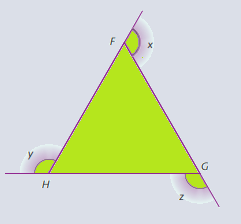
\includegraphics[width=1.88333in,height=1.75048in]{./imgSAEB_8_MAT/media/image13.png}
\end{figure}

\begin{multicols}{3}
\begin{escolha}[itemsep=0pt]
\item os vértices do triângulo;
        \rosa{$F, G$ e $H$}
\item os lados do triângulo;
        \rosa{$FH, FG$ e $HG$}
\item os ângulos internos do triângulo;
        \rosa{$F, G$ e $H$}
\item os ângulos externos do triângulo;
        \rosa{$x, y$ e $z$}
\item o lado oposto ao ângulo F
        \rosa{$HG$}
\end{escolha}
\end{multicols}




\num{2} No triângulo representado a seguir, AD é a bissetriz em relação a
BÂC. Determine o valor de x, em graus.

\begin{figure}[H]
\centering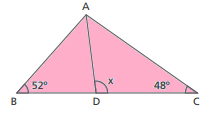
\includegraphics[width=2.20833in,height=1.1875in]{./imgSAEB_8_MAT/media/image14.png}
\end{figure}

\reduline{ Considerando a soma dos ângulos internos, temos que: $52 + 48 = 100$\hfill}\\
\reduline{ Logo, o ângulo $BAC = 80°$, e o valor de sua bissetriz é $40°$. Assim, o ângulo x possui:\hfill}\\
\reduline{ $40 + 48 = 88$ e $180 - 88 = 92°$.\hfill}\\

\num{3} Em cada caso descrito, analise se é possível construir um triângulo
com lado BC de 5 cm e com as medidas dos ângulos indicadas.

\begin{escolha}
\item medida do ângulo $(B)= 110° $ e medida do ângulo $(C) = 50°$
\item medida do ângulo $(B) = 110°$ e medida do ângulo $(C)= 70°$
\item medida do ângulo $(B) = 110°$ e medida do ângulo $(C) = 90°$
\end{escolha}

\reduline{ Considerando que a soma dos ângulos internos do triângulo deve ser\hfill}\\
\reduline{ $180$, chegamos à conclusão de que é possível.\hfill}\\
\reduline{ Considerando que a soma dos ângulos internos do triângulo deve ser\hfill}\\
\reduline{ $180$, chegamos à conclusão de que não é possível.\hfill}\\
\reduline{ Considerando que a soma dos ângulos internos do triângulo deve ser\hfill}\\
\reduline{ $180$, chegamos à conclusão de que não é possível.\hfill}\\

\pagebreak
\num{4} Em cada triângulo representado a seguir, onde foram traçadas algumas
retas, identifique se o ponto O é circuncentro, incentro, baricentro ou
ortocentro.
\begin{multicols}{2}
\begin{escolha}
\item
\begin{figure}[H]
\centering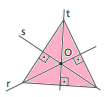
\includegraphics[width=4cm]{./imgSAEB_8_MAT/media/image15.png}
\end{figure} \rosa{Ortocentro}
\item
\begin{figure}[H]
\centering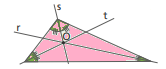
\includegraphics[width=4cm]{./imgSAEB_8_MAT/media/image16.png}
\end{figure} \rosa{Incentro}
\item
\begin{figure}[H]
\centering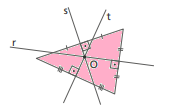
\includegraphics[width=4cm]{./imgSAEB_8_MAT/media/image17.png}
\end{figure} \rosa{Circuncentro}
\item
\begin{figure}[H]
\centering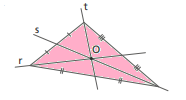
\includegraphics[width=4cm]{./imgSAEB_8_MAT/media/image18.png}
\end{figure} \rosa{Baricentro}
\end{escolha}
\end{multicols}


\num{5} Em cada item, verifique se os triângulos são congruentes:


\begin{multicols}{2}
\begin{escolha}
\item
\begin{figure}[H]
\centering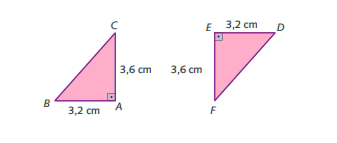
\includegraphics[width=4cm]{./imgSAEB_8_MAT/media/image19.png}
\end{figure}  \rosa{São congruentes}
\item
\begin{figure}[H]
\centering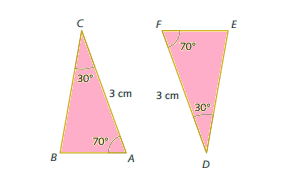
\includegraphics[width=4cm]{./imgSAEB_8_MAT/media/image20.png}
\end{figure}  \rosa{São congruentes}
\item
\begin{figure}[H]
\centering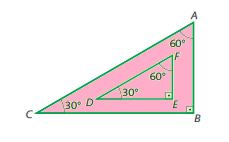
\includegraphics[width=4cm]{./imgSAEB_8_MAT/media/image21.png}
\end{figure}  \rosa{Não são congruentes}
\item
\begin{figure}[H]
\centering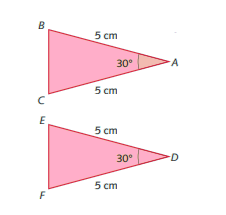
\includegraphics[width=4cm]{./imgSAEB_8_MAT/media/image22.png}
\end{figure}  \rosa{São congruentes}
\item
\begin{figure}[H]
\centering
\includegraphics[width=4cm]{./imgSAEB_8_MAT/media/image23.png}
\end{figure}  \rosa{São congruentes}
\end{escolha}
\end{multicols}





\num{6} Calcule, em graus, as medidas dos ângulos dos triângulos abaixo:

\begin{multicols}{2}
\begin{escolha}
\item
\begin{figure}[H]
\centering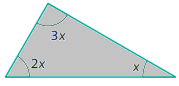
\includegraphics[width=4cm]{./imgSAEB_8_MAT/media/image24.png}
\end{figure}
\item
\begin{figure}[H]
\centering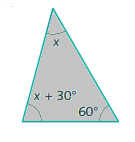
\includegraphics[width=4cm]{./imgSAEB_8_MAT/media/image25.png}
\end{figure}
\item
\begin{figure}[H]
\centering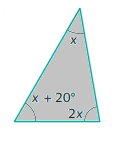
\includegraphics[width=4cm]{./imgSAEB_8_MAT/media/image26.png}
\end{figure}
\item
\begin{figure}[H]
\centering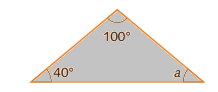
\includegraphics[width=4cm]{./imgSAEB_8_MAT/media/image27.png}
\end{figure}
\item
\begin{figure}[H]
\centering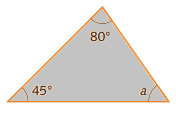
\includegraphics[width=4cm]{./imgSAEB_8_MAT/media/image28.png}
\end{figure}
\item
\begin{figure}[H]
\centering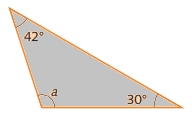
\includegraphics[width=4cm]{./imgSAEB_8_MAT/media/image29.png}
\end{figure}
\end{escolha}
\end{multicols}

\reduline{ a) $ 3x + 2x + x = 180; 6x = 180; x = 30. Logo, os respectivos ângulos são 30°,60° e 90°.$\hfill}\\
\reduline{ b) $x + x + 30 + 60 = 180; 2x + 90 = 180; 2x = 90; x = 45$\hfill}\\
\reduline{ Log$o, os ângulos são 45°, 75° e 60°.$\hfill}\\
\reduline{ c) $x + x + 20 + 2x = 180; 4x + 20 = 180; 4x = 160; x = 40$\hfill}\\
\reduline{ Log$o, os ângulos são respectivamente 40°, 60° e 80°$\hfill}\\
\reduline{ d) $a = 40°; e) a = 55° f) a = 108°$\hfill}\\

\pagebreak

\num{7} Determine as medidas do ângulo complementar e do ângulo suplementar
de cada ilustração a seguir:

\begin{figure}[H]
\centering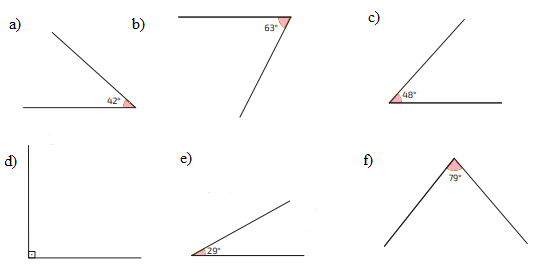
\includegraphics[width=4.81667in,height=2.48373in]{./imgSAEB_8_MAT/media/image30.png}
\end{figure}
\reduline{ $48° e 138°; 27° e 117°; 42° e 132°; 0° e 90°; 61° e 151°; 11° e 101°$.\hfill}\\

\num{8} Ao folear um livro de engenharia de seu pai, Marcos se deparou com a
seguinte imagem:

\begin{figure}[H]
\centering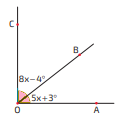
\includegraphics[width=1.47134in,height=1.42708in]{./imgSAEB_8_MAT/media/image31.png}
\end{figure}

Para encontrar o valor de $x$, quais os passos Enzo deve tomar?

\reduline{ Observar que o ângulo destacado é igual a $90°$.\hfill}\\
\reduline{ Montar a equação da seguinte forma:\hfill}\\
\reduline{ $8x - 4 + 5x + 3 = 90$\hfill}\\
\reduline{ $13x - 1 = 90$\hfill}\\
\reduline{ $13x = 91$\hfill}\\
\reduline{ $x = 7$\hfill}\\

\pagebreak

\num{9} Calcule as medida do ângulos destacados abaixo, considerando que as
linhas em verde traçam a bissetriz de cada ângulo.

\begin{figure}[H]
\centering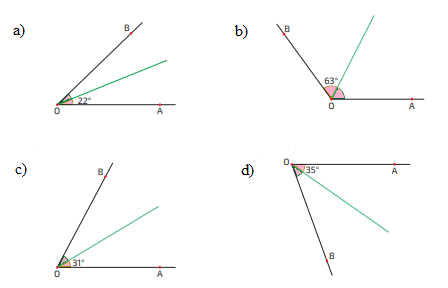
\includegraphics[width=4.66667in,height=3in]{./imgSAEB_8_MAT/media/image32.png}
\end{figure}

\reduline{ $44°, 126°, 62° e 70°$.\hfill}\\

\num{10} Calcule o valor de $x$ nas figuras abaixo.

\begin{multicols}{2}
\begin{escolha}
\item
\begin{figure}[H]
\centering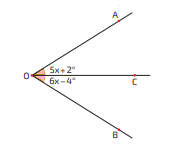
\includegraphics[width=1.91667in,height=1.6875in]{./imgSAEB_8_MAT/media/image33.png}
\end{figure}  \rosa{$5x + 2 = 6x - 4; -x = -6; x = 6$}
\item
\begin{figure}[H]
\centering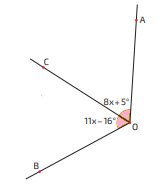
\includegraphics[width=1.80208in,height=2.02917in]{./imgSAEB_8_MAT/media/image34.png}
\end{figure}  \rosa{$11x - 16 = 8x + 5$; $3x = 21$; $x = 7$}
\end{escolha}
\end{multicols}

\pagebreak

\section{Treino}

\num{1} Denomina-se incentro o ponto comum

\begin{escolha}[itemsep=0pt]
\item às alturas do triângulo;
\item às mediatrizes dos lados do triângulo;
\item às medianas do triângulo;
\item às bissetrizes do triângulo. 
\end{escolha}

% SAEB: Resolver problemas que envolvam relações entre ângulos formados
% por retas paralelas cortadas por uma transversal, ângulos internos ou
% externos de polígonos ou cevianas (altura, bissetriz, mediana,
% mediatriz) de polígonos.

% BNCC: EF08MA14 -- Demonstrar propriedades de quadriláteros por meio da
% identificação da congruência de triângulos.

% A: Incorreta, pois essa definição de incentro está errada.

% B: Incorreta, pois essa definição de incentro está errada.

% C: Incorreta, pois essa definição de incentro está errada.

% D: Correta, pois as bissetrizes do triângulo correspondem ao incentro.

\num{2} O triângulo ABC é um triângulo retângulo em A e isósceles. O ponto O
é o seu circuncentro, ou seja, é o centro da circunferência circunscrita
ao triângulo. Se a altura relativa à hipotenusa BC mede $9,3\,cm$, qual é a
medida da hipotenusa?

\begin{figure}[H]
\centering
\includegraphics[width=2.5625in,height=2.02083in]{./imgSAEB_8_MAT/media/image35.png}
\end{figure}

\begin{escolha}[itemsep=0pt]
\item 9,3
\item 18,2
\item 18,6 
\item 18,8
\end{escolha}

% SAEB: Resolver problemas que envolvam relações entre ângulos formados
% por retas paralelas cortadas por uma transversal, ângulos internos ou
% externos de polígonos ou cevianas (altura, bissetriz, mediana,
% mediatriz) de polígonos.

% BNCC: EF08MA14 -- Demonstrar propriedades de quadriláteros por meio da
% identificação da congruência de triângulos.

% A: Incorreta, pois esse seria o valor relativo, e não a medida final.

% B: Incorreta, pois houve um erro na multiplicação.

% C: Correta, pois, se a altura relativa à hipotenusa BC mede 9,3\,cm, a
% medida da hipotenusa será 18,6.

% D: Incorreta, pois o aluno chegará a essa conclusão ao errar o cálculo
% de multiplicação dos termos destacados no enunciado.

\num{3} Qual é o perímetro de um triângulo com lados cujas medidas são $6 cm$,
$7 cm$ e $8 cm$?

\begin{escolha}[itemsep=0pt]
\item $19 cm$
\item $20 cm$
\item $21 cm$ 
\item $22 cm$
\end{escolha}






% SAEB: Identificar propriedades e relações existentes entre os elementos
% de um triângulo (condição de existência, relações de ordem entre as
% medidas dos lados e as medidas dos ângulos internos, soma dos ângulos
% internos, determinação da medida de um ângulo interno ou externo)

% BNCC: EF08MA14 -- Demonstrar propriedades de quadriláteros por meio da
% identificação da congruência de triângulos.

% A: Incorreta, pois o aluno chegará a essa conclusão se, durante o
% cálculo da soma dos lados do triangulo, encontrar 2 números a menos.

% B: Incorreta, pois o aluno chegará a essa conclusão se, durante o
% cálculo da soma dos lados do triangulo, encontrar 1 número a menos.

% C: Correta, pois:

% Perímetro = soma dos lados, logo 6 + 7 + 8 = 21 cm

% D: Incorreta, pois o aluno chegará a essa conclusão se, durante o
% cálculo da soma dos lados do triangulo, encontrar 1 número a mais.


\chapter{Representações espaciais}

\begin{itemize}
  \item Descrever ou esboçar deslocamento de pessoas e/ou de objetos em
  \item representações bidimensionais (mapas, croquis etc.), plantas de
  \item ambientes ou vistas, de acordo com condições dadas.
\end{itemize}


\subsection{Habilidade da BNCC}

\begin{itemize}
\item EF08MA25.
\end{itemize}

\conteudo{
\smallskip\noindent\textbf{Mapas}
\quad
Um mapa é uma representação gráfica ou diagrama de uma área geográfica
específica, seja ela uma região, um país, um continente ou até mesmo o
mundo inteiro. Ele é projetado para mostrar a localização relativa de
diferentes elementos geográficos, como cidades, estradas, rios,
montanhas e outros recursos naturais e artificiais.

Os mapas podem ser apresentados em diferentes projeções, que são métodos
de representação tridimensional da Terra em uma superfície
bidimensional. As projeções ajudam a minimizar distorções e deformações
causadas pela transferência de uma esfera para um plano.

\smallskip\noindent\textbf{Croquis}
\quad
Um croqui é um tipo de representação gráfica ou esboço rápido e informal
que visa capturar a essência visual ou a forma básica de algo, como um
objeto, um local ou uma ideia. É geralmente um desenho simples,
esquemático e sem muitos detalhes, que serve como um registro visual
rápido e simplificado.

Os croquis são frequentemente usados em diversas áreas, como
arquitetura, design de interiores, design de moda, planejamento urbano,
desenho industrial, arte e até mesmo em anotações pessoais. Eles são uma
maneira rápida e eficiente de visualizar e comunicar ideias
preliminares, conceitos ou esboços iniciais.

\smallskip\noindent\textbf{Deslocamento}
\quad
O deslocamento pode ser considerado a distância percorrida por um objeto
ou alguém durante um período de tempo. Essa distância pode ser
representada pela fórmula:
Distância = velocidade média x tempo.}

\section{Atividades}

\num{1} Paulo está pretendendo fazer uma longa viagem para visitar seus pais.

\begin{figure}[H]
\centering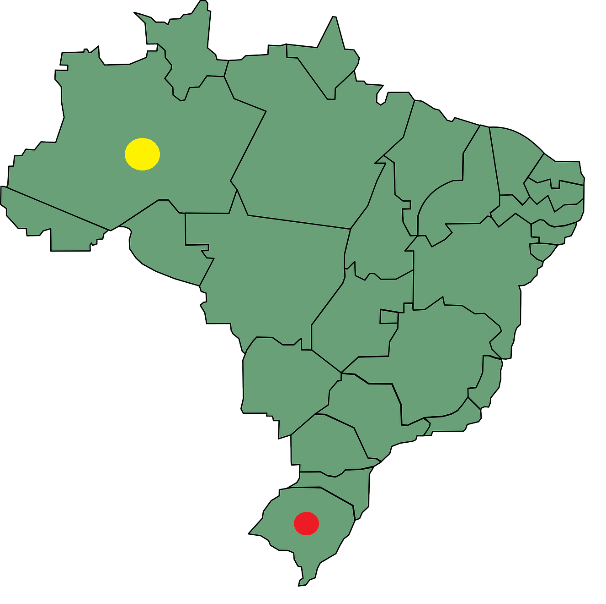
\includegraphics[width=2.73952in,height=2.725in]{./imgSAEB_8_MAT/media/image36.png}
\end{figure}

% Disp$onível em:
% \url{https://pixabay.com/pt/vectors/brasil-mapa-am\%c3\%a9rica-do-sul-estados-23553/}.
% Acesso em: 23 maio 2023.$

Considerando que a casa de Paulo está demarcada com a esfera vermelha e
a casa de seus pais com a esfera amarela, qual é o número mínimo de
estados que Paulo vai ter que atravessar para ver seus pais?

\reduline{ Paulo atravessará, no mínimo, 4 estados até chegar à casa de seus pais.\hfill}
\linhas{3}

\num{2} A circunferência da Terra possui 40.075\,km de extensão. Suponhamos
que Júlio queira dar uma volta ao mundo em 80 dias com o seu barco. Qual
deslocamento diário aproximado que deverá percorrer para cumprir seu
objetivo?

\reduline{ Considerando que a terra possui 40.075 km de extensão e a viagem deverá\hfill}\\
\reduline{ durar, no máximo, 80 dias:\hfill}\\
\reduline{ 40.075 km \div 80 dias = aproximadamente 501 km por dia.\hfill}
\linhas{3}

\pagebreak

\num{3} Francisco estava em casa e resolveu convidar sua namorada para jantar
fora. Para facilitar o deslocamento, ele encaminhou um mapa da
trajetória.



\begin{figure}[H]
\centering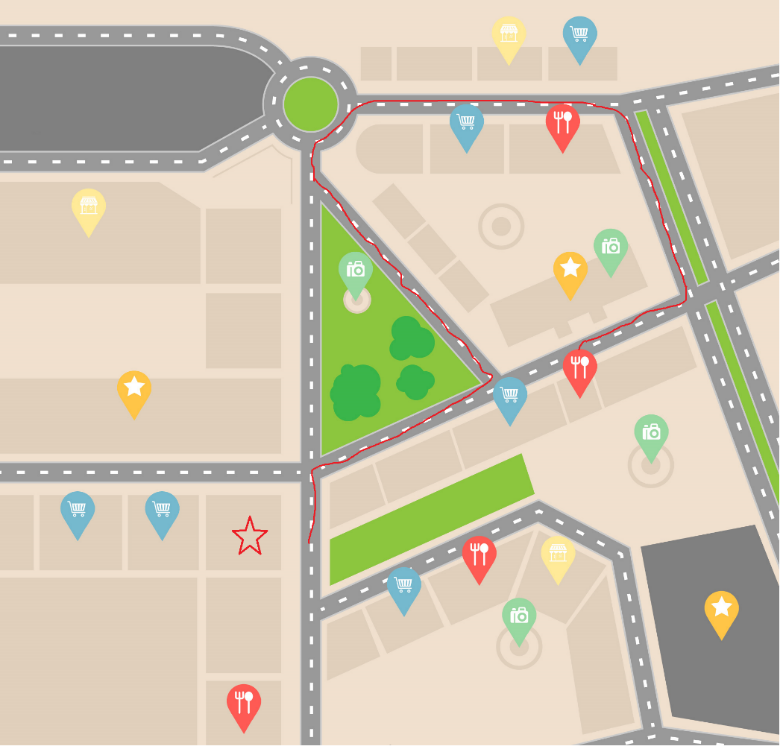
\includegraphics[width=3.55in,height=3.406in]{./imgSAEB_8_MAT/media/image37.png}
\end{figure}

% Disponível em:
% \url{https://br.freepik.com/vetores-gratis/mapa-cidade-apartamento-desenho_1107608.htm\#query=mapas\&position=6\&from_view=search\&track=sph}.
% Acesso em: 23 maio 2023. Adaptado.

Caso ela não consiga abrir a imagem, como ele poderia descrever o
caminho?

\reduline{ Ao sair da Residência de Francisco, pegue a primeira rua à direita,\hfill}\\
\reduline{ depois vire à esquerda, depois entre \hfill}\\
\reduline{ na rotatória e saia na primeira\hfill}\\
\reduline{ saída e siga em frente, depois vire à direita na avenida e finalment vire à direita.}\\

\num{4} Em uma tarde de domingo, João estava entediado e resolveu dar um
passeio na roda gigante de sua cidade.

\begin{figure}[H]
\centering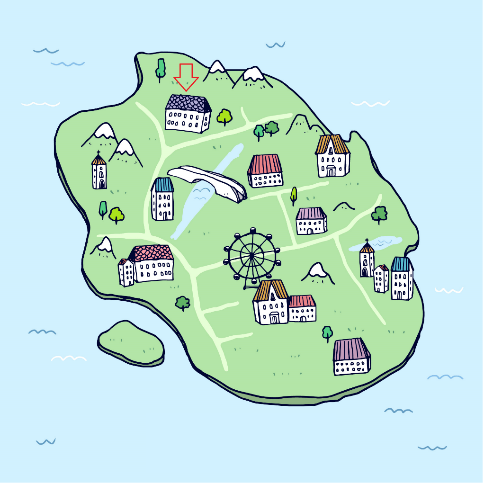
\includegraphics[width=2.2in,height=2.2in]{./imgSAEB_8_MAT/media/image38.png}
\end{figure}

%Disponível em:
%\url{https://br.freepik.com/vetores-gratis/mao-desenhado-cidade-mapa-ferris-roda_1106040.htm\#query=mapa\%20feito\%20a\%20m\%C3\%A3o\&position=6\&from_view=search\&track=ais}.
%Acesso em 23 maio 2023.

Considerando que João mora na casa marcada com a seta no mapa, qual
trajeto até a roda gigante pode ser traçado?

\reduline{ João pode chegar até a roda gigante por dois caminhos. O primeiro,\hfill}\\
\reduline{ pegando a estrada à direita da sua casa e seguindo nela até virar à\hfill}\\
\reduline{ esquerda na estrada da roda gigante.\hfill}\\
\reduline{ O segundo, passando pela ponte à direita de sua casa, atravessando pela\hfill}\\
\reduline{ ponte e seguindo na estrada, virando à direita após atravessar a ponte e\hfill}\\
\reduline{ finalmente virar à esquerda.\hfill}\\

\num{5} Considerando que a distância entre a terra e a lua é de $384.400\,km$,
qual é o deslocamento total percorrido por um astronauta que pisa no
satélite natural e retorna ao planeta?

\reduline{ $384.400$ na ida $+ 384.400$ na volta $=$ deslocamento total $= 768.400 km$.\hfill}
\linhas{3}


\num{6} Lia está fazendo um test drive com um carro de uma concessionária. Ao
sair, recebeu as seguintes dicas do GPS:

\begin{enumerate}[itemsep=0pt]
\item Siga em frente  $100 m$
\item Vire à esquerda $200 m$
\item Vire à esquerda $200 m$
\item Vire à esquerda $200 m$
\item Vire à esquerda $100 m$
\end{enumerate}

Ao receber essas informações, pode-se afirmar que aconteceu o quê?

\reduline{ Lia voltou à concessionária.\hfill}\\

\num{7} Marcelo e amigos estavam indo para praia. No meio do caminho,
perceberam que esqueceram a bagagem em casa. Assim, resolveram voltar
para pegá-la e, enfim, seguir viagem.

Considerando que a distância entre a casa e a praia seja de $300 km$, qual
é o deslocamento total de Marcelo e seus amigos até chegarem à praia?

\reduline{ Considerando que já estavam na metade do caminho, percorreram $150 km + a$\hfill}\\
\reduline{ viagem completa de $300km$, ou seja, temos que $150 km + 300 km = 450 km$.\hfill}

\pagebreak

\num{8} Cléber é motorista de ônibus de uma metrópole brasileira. Sua linha
anda por 3 bairros diferentes em um percurso total de 32 km. Sabendo que
Cléber trabalha das 6 horas da manhã até as 16 horas e realiza esse
percurso 4 vezes, qual é o descolamento diário de Cléber no trabalho?

\reduline{ 32 km cada percurso, Cléber realiza o percurso 4 vezes por dia; \hfill}\\
\reduline{ logo, temos que $4 \cdot 32 km = 128 km$ por dia.\hfill}\\
\linhas{2}

\num{9} Marina vai ao trabalho de carro de segunda a sexta. A distância da
casa de marina até seu trabalho é de 12 km. Sabendo que seu carro gasta
0,50 centavos de gasolina a cada 1 km, qual é o valor total que Marina
gasta com combustível durante a semana?

\reduline{ $12 km$ para ir e $12 km$ para voltar $= 24 km$ diários.\hfill}
\linhas{3}

Logo, se a cada 1 km Marina gasta 0,50 centavos, temos que, em 24 km,
ela gasta R\$\,12,00.

Contando 5 dias trabalhados na semana, $12 \cdot 5 =$ R\$\,60,00 por semana.

\num{10} Em um livro infantil, um menino sai vagando pelo espaço, de planeta
em planeta, caçando novas aventuras. Considerando que, durante a
história do livro, ele tenha visitado 8 planetas, e que a distância
entre cada planeta seja de $(10^5)$ km, qual foi o deslocamento que o
menino da história realizou?

\reduline{ Considerando 8 planetas, temos que:\hfill}\\
\reduline{ $8 x (10^5)$\hfill}\\
\reduline{ $8 \cdot 100.000 = 800.000 km$\hfill}\\
\linhas{1}

\pagebreak

\section{Treino}

\num{1} Um jogador de Futebol corre em média 8 km por partida. Considerando
que um campeonato tenha 38 rodadas e que esse jogador jogue todas as
partidas, qual é deslocamento total durante o campeonato?

\begin{escolha}[itemsep=0pt]
\item $8 km$ por campeonato
\item $38 km$ por campeonato
\item $30,4 km$ por campeonato
\item $304 km$ por campeonato \rosa{-- X}
\end{escolha}

% Habilidade SAEB: Descrever ou esboçar deslocamento de pessoas e/ou de
% objetos em representações bidimensionais (mapas, croquis etc.), plantas
% de ambientes ou vistas, de acordo com condições dadas.

% A: Incorreta, pois, ao considerar que o enunciado pede o valor de km por
% partida, o aluno pode chegar a essa conclusão.

% B: Incorreta, pois ao considerar a quantidade de rodadas ao invés da
% quantidade de km percorridos, o aluno pode chegar a esse valor.

% C: Incorreta, pois, ao deslocar erroneamente uma vírgula para a
% esquerda, o aluno pode chegar a esse resultado.

% D: Correta, pois

% 8 km x 38 partidas = 304 km por campeonato.

\num{2} A velocidade de uma baleia azul pode chegar a 50 km/h. Considerando
que uma baleia esteja a navegar pelo mar em sua velocidade máxima, e que
nade por 8 horas ininterruptas, qual é seu deslocamento total?

\begin{escolha}[itemsep=0pt]
\item $40 km$
\item $4.000 km$
\item $400 km$ \rosa{-- X}
\item $40.000 km$
\end{escolha}

% SAEB: Descrever ou esboçar deslocamento de pessoas e/ou de objetos em
% representações bidimensionais (mapas, croquis etc.), plantas de
% ambientes ou vistas, de acordo com condições dadas.

% A: Incorreta, pois esse seria o valor caso o aluno realizasse
% incorretamente a multiplicação.

% B: Incorreta, pois esse seria o valor caso o aluno realizasse
% incorretamente a multiplicação, adicionando um ``zero'' na expressão.

% C: Correta pois:

% (\frac{50}{x} = \frac{1}{8})

% 50 \cdot 8 = x

% 400 km.

% D: Incorreta, pois esse seria o valor caso o aluno realizasse
% incorretamente a multiplicação, adicionando dois ``zeros'' na expressão.

\num{3} Charles é um botânico de renome e, ao sair para realizar pesquisas em
uma floresta, acabou se perdendo no meio da mata. Ele também esqueceu
seus equipamentos de navegação em seu laboratório, e a única coisa de
que se lembra é que a cidade mais próxima fica ao rumo do pôr sol. Para
chegar à cidade mais próxima, para qual sentido Charles deve andar?

\begin{escolha}[itemsep=0pt]
\item Norte
\item Sul
\item Leste
\item Oeste \rosa{-- X}
\end{escolha}

% SAEB: Descrever ou esboçar deslocamento de pessoas e/ou de objetos em
% representações bidimensionais (mapas, croquis etc.), plantas de
% ambientes ou vistas, de acordo com condições dadas.

% A: Incorreta, pois o aluno pode se confundir em relação aos pontos
% cardeais.

% B: Incorreta, pois o aluno pode se confundir em relação aos pontos
% cardeais.

% C: Incorreta, pois o aluno pode se confundir em relação aos pontos
% cardeais.

% D: Correta, pois Charles deve seguir rumo ao Oeste.


\chapter{Introdução à estatística}

\section{Habilidades do SAEB}

\begin{itemize}
\item Identificar os indivíduos (universo ou
população-alvo da pesquisa), as variáveis e os tipos de variáveis
(quantitativas ou categóricas) em um conjunto de dados.
\item
  Representar ou associar os dados de uma pesquisa estatística ou de um
  levantamento em listas, tabelas (simples ou de dupla entrada) ou
  gráficos (barras simples ou agrupadas, colunas simples ou agrupadas,
  pictóricos, de linhas, de setores, ou em histograma).
\item
  Inferir a finalidade da realização de uma pesquisa estatística ou de
  um levantamento, dada uma tabela (simples ou de dupla entrada) ou
  gráfico (barras simples ou agrupadas, colunas simples ou agrupadas,
  pictóricos, de linhas, de setores ou em histograma) com os dados dessa
  pesquisa.
\item
  Interpretar o significado das medidas de tendência central (média
  aritmética simples, moda e mediana) ou da amplitude.
\item
  Calcular os valores de medidas de tendência central de uma pesquisa
  estatística (média aritmética simples, moda ou mediana).
\item
  Resolver problemas que envolvam dados estatísticos apresentados em
  tabelas (simples ou de dupla entrada) ou gráficos (barras simples ou
  agrupadas, colunas simples ou agrupadas, pictóricos, de linhas, de
  setores ou em histograma).
\item
  Argumentar ou analisar argumentações/conclusões com base nos dados
  apresentados em tabelas (simples ou de dupla entrada) ou gráficos
  (barras simples ou agrupadas, colunas simples ou agrupadas,
  pictóricos, de linhas, de setores ou em histograma).
\item
  Explicar/descrever os passos para a realização de uma pesquisa
  estatística ou de um levantamento.
\end{itemize}

\subsection{Habilidade da BNCC}

\begin{itemize}
\item EF08MA25.
\end{itemize}


\conteudo{
\smallskip\noindent\textbf{Conceitos básicos da Estatística}
\quad
A Estatística é uma área da Matemática voltada ao estudo de métodos para
coleta, organização e análise de dados, visando à tomada de decisões.
Realizamos uma pesquisa estatística quando pretendemos estudar alguma
característica de determinado conjunto de elementos. O conjunto de todos
os elementos analisados na pesquisa é denominado população. Quando temos
muitos elementos na população que queremos estudar, podemos selecionar
uma amostra representativa.

População é o conjunto de elementos que queremos pesquisar e que
apresentam alguma característica comum.

\smallskip\noindent\textbf{Amostra é um subconjunto da população.}
\quad
Algumas pesquisas exigem a investigação de toda uma população. Esse tipo
de pesquisa é denominada censitária.

\smallskip\noindent\textbf{Amostra casual simples}
\quad
A amostra casual simples é caracterizada por um sorteio aleatório. Os
elementos de uma população podem ser enumerados e, em seguida, sorteados
entre uma quantidade estabelecida previamente.

\smallskip\noindent\textbf{Amostra sistemática}
\quad
No caso da amostra sistemática, os elementos da população a ser estudada
já se encontram ordenados. Por exemplo: produtos de uma linha de
produção, prontuários médicos, prédios de uma rua etc. Para a seleção
dos elementos que farão parte da amostra, é elaborado um sistema pelo
pesquisador.

\smallskip\noindent\textbf{Amostra proporcional estratificada}
\quad
Na amostra estratificada, a população é dividida em subpopulações
denominadas estratos. Esse tipo de amostra é realizado quando outras
características da população devem ser levadas em conta. Por exemplo,
nas pesquisas de intenção de voto para presidente do Brasil, a população
são os eleitores brasileiros, mas a região do país onde eles residem,
seu sexo, sua faixa etária e sua faixa de renda são dados importantes.
Assim, o pesquisador deve selecionar uma amostra aleatória de cada
estrato.

\smallskip\noindent\textbf{Variáveis}
\quad
As variáveis são as características que analisadas em uma amostra ou
população. Elas podem assumir valores numéricos e não numéricos, sendo
classificadas em qualitativas e quantitativas.

\smallskip\noindent\textbf{Organização dos dados}
\quad
Para organizar os dados obtidos por meio de uma pesquisa, podemos
construir tabelas e gráficos. O tipo de tabela e de gráfico que vamos
utilizar é condicionado pela variável analisada.

\smallskip\noindent\textbf{Média aritmética}
\quad
A média aritmética simples de uma série de dados é determinada pela soma
de todos os dados dividida pela quantidade de dados.

\smallskip\noindent\textbf{Moda}
\quad
A moda de uma série de dados é determinada pelo valor que apresenta a
maior frequência.

\smallskip\noindent\textbf{Mediana}
\quad
A mediana é a medida estatística que divide o conjunto de dados em duas
partes com a mesma quantidade de termos. Enquanto a primeira parte
apresenta valores menores ou iguais a ela, a segunda parte é formada por
valores maiores.}

\section{Atividades}

\num{1} Leia o gráfico a seguir e responda.

\begin{figure}[H]
\centering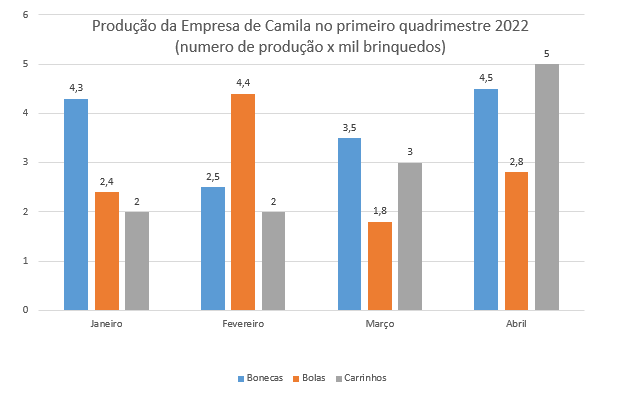
\includegraphics[width=5.90625in,height=3.86458in]{./imgSAEB_8_MAT/media/image39.png}
\end{figure}

\begin{escolha}[itemsep=0pt]
\item O mês em que houve a maior quantidade de brinquedos produzidos foi:
\item O mês em que houve a menor quantidade de produção:
\item O brinquedo mais produzido foi:
\item O brinquedo menos foi produzido foi:
\item Quantos brinquedos ao total a empresa de Camila produziu no primeiro quadrimestre de 2022?
\end{escolha}

\reduline{ Abril\hfill}\\
\reduline{ Março\hfill}\\
\reduline{ Os brinquedos mais produzidos foram as Bonecas\hfill}\\
\reduline{ Os brinquedos menos reproduzidos foram as bolas\hfill}\\
\reduline{ Realizando a soma dos dados do gráfico, obtemos que a empresa de Camila fabricou um total de 38.400 brinquedos.\hfill}\\

\num{2} Ronaldo resolveu colocar em um gráfico todos os custos mensais de sua casa.

\begin{figure}[H]
\centering
\includegraphics[width=5.30833in,height=3.41384in]{./imgSAEB_8_MAT/media/image40.png}
\end{figure}

Ao analisar o gráfico, responda.

\begin{escolha}[itemsep=0pt]
\item Ronaldo comprou um ar-condicionado que consome muita energia. Qual foi o mês da compra?
\item A filha de Ronaldo contratou um plano adicional de internet. Qual foi o mês da aquisição?
\item Qual conta nunca apresentou uma grande alta de valor?
\item Em que mês Ronaldo pagou o menor valor de contas na sua casa?
\end{escolha}

\reduline{Entre o mês de janeiro e fevereiro.\hfill}\\
\reduline{No mês de maio.\hfill}\\
\reduline{A conta de Água.\hfill}\\
\reduline{Janeiro.\hfill}\\

\pagebreak

\num{3} Poliana está passando por uma reeducação financeira e começou a
dividir seus gastos de forma que ainda sobre um dinheiro para
aproveitar.

\begin{figure}[H]
\centering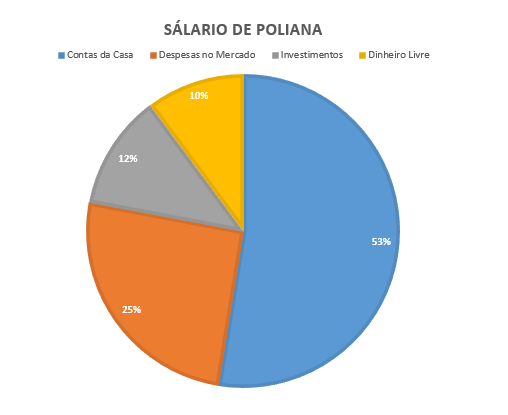
\includegraphics[width=3.65in,height=2.98179in]{./imgSAEB_8_MAT/media/image41.png}
\end{figure}

Considerando que o salário mensal de Poliana é R\$\,3.000,00, responda.

\begin{escolha}[itemsep=0pt]
\item Qual é o valor destinado mensalmente para as contas da casa?
\item Qual é o valor destinado mensalmente para despesas no mercado?
\item Qual é o valor destinado mensalmente para investimentos?
\item Poliana quer comprar um carro novo no valor de R\$\,30.000,00.
Se Poliana utilizar a parte de investimentos do seu salário, quantos meses
demorará até comprar o carro?
\end{escolha}

\rosa{a) $3.000 \cdot 0,53 = R\$\,1.590,00$}
\rosa{b) $3.000 \cdot 0,25 = R\$\,750,00$}
\rosa{c) $3.000 \cdot 0,12 = R\$\,360,00$}
\rosa{d) $30.000 \div 360 = 84$ meses.}

\pagebreak

\num{4} Um professor realizou uma pesquisa com sua turma de matemática para
identificar a altura dos estudantes. Os dados coletados foram os
seguintes (em centímetros): $150, 165, 160, 155, 170, 160, 160, 165, 155, 165$ 


Calcule a média aritmética simples, a moda e a mediana das alturas dos
estudantes.

\reduline{ Média aritmética simples:\hfill}\\
\reduline{ $(150 + 165 + 160 + 155 + 170 + 160 + 160 + 165 + 155 + 165) / 10 = 159,5 cm$\hfill}\\
\reduline{ Para encontrar a moda, identificamos o valor que mais se repete. Nesse\hfill}\\
\reduline{ caso, temos duas alturas que se repetem mais vezes, que são $160 cm$ e $165$\hfill}\\
\reduline{ cm, ambas aparecendo três vezes. Portanto, a moda das alturas dos\hfill}\\
\reduline{ estudantes é $160 cm$ e $165 cm$.\hfill}\\
\reduline{ Para encontrar a mediana, ordenamos os valores em ordem crescente.\hfill}\\
\reduline{ Assim, temos: $150, 155, 155, 160, 160, 160, 165, 165, 165, 170$\hfill}\\
\reduline{ Como temos um número ímpar de dados (10), a mediana será o valor\hfill}\\
\reduline{ central. Nesse caso, a mediana das alturas dos estudantes é $160 cm$.\hfill}\\

\num{5} Um professor deseja calcular a média aritmética das notas finais de
seus alunos em uma disciplina. Ele possui os seguintes dados das notas
dos alunos: $7, 8, 6, 9, 5, 8, 7, 6$.

Calcule a média aritmética simples das notas dos alunos e explique a
resposta.

\reduline{Para calcular a média aritmética simples das notas dos alunos, devemos
somar todas as notas e dividir pelo número total de alunos.
Passo 1: somar as notas $7 + 8 + 6 + 9 + 5 + 8 + 7 + 6 = 56$
Passo 2: dividir pelo número total de alunos $56 / 8 = 7$
A média aritmética simples das notas dos alunos é igual a 7.\hfill}

\num{6} Uma empresa está realizando uma pesquisa sobre o nível de satisfação
de seus funcionários. Para isso, foi feito um levantamento com 35
colaboradores dos 300 registrados na empresa. Com base nas informações
anteriores, responda:


\begin{escolha}[itemsep=0pt]
\item Qual é a população dessa pesquisa?
\item Qual é a sua amostra?
\end{escolha}

\reduline{Os 300 funcionários registrados.\hfill}
\reduline{35 funcionários.\hfill}

\pagebreak

\num{7} O quadro mostra algumas notas de Matemática de alguns alunos do oitavo ano.

%Paulo, criar uma tabela com as informações abaixo:

\begin{longtable}[]{@{}lllll@{}}
\toprule
Notas da disciplina Matemática & & & &\tabularnewline
\midrule
\endhead
Alunos & 1° bimestre & 2° bimestre & 3° bimestre & 4°
bimestre\tabularnewline
Adriana & 7 & 6,5 & 9 & 8\tabularnewline
Bruno & 3 & 5 & 6 & 5\tabularnewline
Carla & 9 & 9 & 8 & 9\tabularnewline
José & 10 & 8 & 8 & 8\tabularnewline
Renata & 5 & 4 & 5 & 3\tabularnewline
\bottomrule
\end{longtable}

Sobre as notas, responda:

\begin{escolha}
\item Qual é a média aritmética das notas que Adriana obteve nos 4
bimestres?
\item Qual é a média aritmética das notas que Bruno obteve nos 4 bimestres?
\item Qual é a média aritmética das notas que Carla obteve nos 4 bimestres?
\item Qual é a média aritmética das notas que José obteve nos 4 bimestres?
\item Qual é a média aritmética das notas que Renata obteve nos 4
bimestres?
\item Sabendo que, para ser aprovado na disciplina, a média das notas dos 4
bimestres devem ser maior que 6, quais alunos foram aprovados? Quais
foram reprovados?
\end{escolha}

\reduline{$7 + 6,5 + 9 + 8 = 30,5; 30,5 \div 4 = 7,625$\hfill}\\
\reduline{$3 + 5 + 6 + 5 = 19; 19 \div 4 = 4,75$\hfill}\\
\reduline{$9 + 9 + 8 + 9 = 35; 35 \div 4 = 8,75$\hfill}\\
\reduline{$10 + 8 + 8 + 8 = 34; 34 \div 4 = 8,5$\hfill}\\
\reduline{$5 + 4 + 5 + 3 = 17; 17 \div 4 = 4,25$\hfill}\\
\reduline{Bruno e Renata foram reprovados.\hfill}

\num{8} Dona Catarina, de 82 anos, tem 5 irmãs: Genoveva, de 79 Anos,
Clotilde, de 75, Amélia, de 70, Irene, de 67, e Tereza, de 64. Qual é a
média de idade de todas as irmãs?

\reduline{ $82 + 79 + 75 + 70 + 67 + 64 = 437$\hfill}\\
\reduline{ $437 \div 6 = 72,83$\hfill}\\

% \num{9} Uma professora resolveu fazer uma pesquisa com seus alunos que
% consistia em apenas 1 pergunta: Qual é o número do seu calçado?

% Ela obteve os seguintes dados:

% %Paulo: inserir uma tabela com os dados abaixo. Pesquisa do Número do
% Calçado de cada Aluno do 8° A\\
% ----------------------------------------------------- ---- ---- ----
% ---- ---- 35 38 40 42 38 40 40 38 40 44 40 37 42 37 42 42 40 44 40 35 38
% 40 39 38 35 38 38 38 44 38 39 38 38 37 40 37

% Ao observar esses dados, qual é a moda dos números dos calçados dos
% alunos?

% R: Ao observar o quadro, temos que

% 3 Alunos calçam 35

% 9 alunos calçam 40

% 4 alunos calcam 42

% 2 alunos calçam 39

% 11 alunos calçam 38

% 3 alunos calcam 44

% Logo, por método de observação, temos que a Moda consiste em calçados
% número 38.

\pagebreak

\num{9} Um supermercado está realizando uma pesquisa sobre o tempo de espera
dos clientes nas filas dos caixas. Foram registrados os seguintes tempos
de espera em minutos: $3, 5, 2, 4, 6, 3, 5, 4, 2, 3$.
Calcule a média aritmética simples do tempo de espera dos clientes e
explique a resposta.

\reduline{ Passo 1: Somar os tempos de espera $3 + 5 + 2 + 4 + 6 + 3 + 5 + 4 + 2 + 3 = 37$.\hfill}\\
\reduline{ Passo 2: Dividir pelo número total de observações $37 / 10 = 3,7$ minutos.\hfill}\\

\section{Treino}

\num{1} Em um jogo de basquete, os 5 atletas de um time que iniciaram o jogo
tinham respectivamente $2,01 m$, $1,99 m$, $2,00 m$, $2,02 m$ e $1,98 m$ de
altura. Qual é a estatura média dessa equipe titular?

\begin{multicols}{2}
\begin{escolha}[itemsep=0pt]
\item $2,02 m$
\item $1,98 m$
\item $2 m$
\item $10 m$
\end{escolha}
\end{multicols}

% SAEB: Calcular os valores de medidas de tendência central de uma
% pesquisa estatística (média aritmética simples, moda ou mediana).

% BNCC: EF08MA25 -- Obter os valores de medidas de tendência central de
% uma pesquisa estatística (média, moda e mediana) com a compreensão de
% seus significados e relacioná-los com a dispersão de dados, indicada
% pela amplitude.

% A: Incorreta, pois o aluno chegaria a esse resultado a partir da maior
% altura da equipe.

% B: Incorreta, pois o aluno chegaria a esse resultado a partir da menor
% altura da equipe.

% C: Correta, pois:

% Somando a altura dos atletas temos:

% 2,01 + 1,99 + 2,00 + 2,02 + 1,98 =10

% Como são 5 atletas

% 10 \div 5 = 2 metros de altura é a média

% D: Incorreta, pois o aluno chegaria a esse resultado a partir da soma
% das alturas da equipe.

\num{2} Um grupo de amigos que frequentam uma academia decidiu compartilhar o
valor de sua última pesagem e chegaram aos seguintes números:

$$46kg, 44kg, 49kg, 45kg, 44kg, 48kg, 50kg, 42kg$$

Qual é a mediana do peso (em quilogramas) desses amigos?

\begin{multicols}{2}
\begin{escolha}[itemsep=0pt]
\item $44kg$
\item $45,5kg$
\item $46 kg$
\item $45kg$
\end{escolha}
\end{multicols}

% SAEB: Calcular os valores de medidas de tendência central de uma
% pesquisa estatística (média aritmética simples, moda ou mediana).

% BNCC: EF08MA25 -- Obter os valores de medidas de tendência central de
% uma pesquisa estatística (média, moda e mediana) com a compreensão de
% seus significados e relacioná-los com a dispersão de dados, indicada
% pela amplitude.

% A: Incorreta, pois o aluno chegaria a esse resultado calculando a moda,
% chegando a uma conclusão equivocada.

% B: Correta, pois:

% Considerando que os dois pesos centrais são 46 e 45 kg,

% 46 + 45 = 91

% 91 \div 2 = 45,5

% C: Incorreta, pois o aluno chegaria a esse resultado calculando a média
% aritmética, e não a mediana.

% D: Incorreta, pois o aluno chegará a esse resultado não levando em
% consideração que, em casos de conteúdos pares, a mediana deve ser a
% média entre os dois valores centrais.

\num{3} Maria caminha todos os dias até seu trabalho. Durante uma semana,
resolveu cronometrar o tempo que leva no trajeto:

\begin{multicols}{2}
\begin{itemize}
\item Segunda-feira: 35 minutos

\item Terça-feira: 32 minutos

\item Quarta-feira: 33 minutos

\item Quinta-feira: 34 minutos

\item Sexta-feira: 36 minutos
\end{itemize}
\end{multicols}

Qual é o tempo médio que Maria gasta para chegar ao trabalho?

\begin{multicols}{2}
\begin{escolha}[itemsep=0pt]
\item 32 minutos
\item 36 minutos
\item 34 minutos
\item 170 minutos
\end{escolha}
\end{multicols}

% SAEB: Calcular os valores de medidas de tendência central de uma
% pesquisa estatística (média aritmética simples, moda ou mediana).

% BNCC: EF08MA25 -- Obter os valores de medidas de tendência central de
% uma pesquisa estatística (média, moda e mediana) com a compreensão de
% seus significados e relacioná-los com a dispersão de dados, indicada
% pela amplitude.

% A: Incorreta, pois o aluno chegaria a esse resultado considerando
% somente o menor tempo gasto.

% B: Incorreta, pois o aluno chegaria a esse resultado considerando
% somente o maior tempo gasto.

% C: Correta, pois:

% Somando o tempo que Maria gastou na semana, temos que:

% 170 minutos / 5 = média de 34 minutos por dia.

% D: Incorreta, pois o aluno chegaria a esse resultado considerando
% somente a soma dos tempos.


\chapter{Perímetro, área e volume}

\section{Habilidades do SAEB}

\begin{itemize}
\item Resolver problemas que envolvam medidas de
grandezas (comprimento, massa, tempo, temperatura, capacidade ou volume)
em que haja conversões entre unidades mais usuais.
\item
  Resolver problemas que envolvam perímetro de figuras planas.
\item
  Resolver problemas que envolvam área de figuras planas.
\item
  Resolver problemas que envolvam volume de prismas retos ou cilindros
  retos.
\end{itemize}

\subsection{Habilidades da BNCC}

\begin{itemize}
\item EF08MA19, EF08MA20, EF08MA21.
\end{itemize}

\conteudo{Para calcularmos o perímetro de uma figura plana, basta realizarmos a
soma de todos os lados da figura.

Já para o cálculo da área de figuras planas, temos de saber fórmulas
específicas para cada tipo de forma. 
Veja alguns exemplos dessas fórmulas:

Área do quadrado: $A = l^2$

Área do triângulo retângulo: $A = (\frac{b.h}{2})$

Área do losango: $A = (\frac{\text{D \cdot d}}{2})$

Área do circulo: $(A = \pi r^{2})$

Área de um retângulo: $(A = l1 \cdot l2)$

Já para o volume, cada poliedro também tem uma fórmula específica. 
Veja alguns exemplos:

Volume de um cubo: $V = l \cdot l \cdot l ou l^3$

Volume de um cilindro $V = (\Pi) \cdot R^2 \cdot h$

Volume de um paralelepípedo: $(V = l1 \cdot l2 \cdot l3)$}

\pagebreak

\section{Atividades}

\num{1} Considere o cubo abaixo.

\begin{figure}[H]
\centering
\includegraphics[width=1.89583in,height=1.27083in]{./imgSAEB_8_MAT/media/image42.png}
\end{figure}

\begin{escolha}[itemsep=0pt]
\item Qual é a medida de perímetro de uma das faces desse cubo?
\item E qual é a medida de área de uma das faces dele?
\item Qual é a medida de volume do cubo?
\end{escolha}

%Deixar o espaço de 2 linhas para resposta em cada item acima.

\reduline{$4 \cdot 3 = 12 cm$\hfill}\\
\reduline{$3 \cdot 3 = 9 cm^2$\hfill}\\
\reduline{$3 \cdot 3 \cdot 3 = 27 cm^3$\hfill}

\num{2} Determine a área de uma região quadrada, sabendo que a medida de
comprimento do lado é de:

\begin{multicols}{2}
\begin{escolha}[itemsep=0pt]
\item $8 cm$
\item $12 cm$
\item $16 m$
\item $20 m$
\item $34 m$
\item $8 mm$
\item $10 mm$
\item $25 mm$
\end{escolha}
\end{multicols}

\reduline{$8 \cdot 8 = 64 cm^2$\hfill}\\
\reduline{$12 \cdot 12 = 144 cm^2$\hfill}\\
\reduline{$16 \cdot 16= 256 m^2$\hfill}\\
\reduline{$20 \cdot 20 = 400 m^2$\hfill}\\
\reduline{$34 \cdot 34= 1156 m^2$\hfill}\\
\reduline{$8 \cdot 8 = 64 mm^2$\hfill}\\
\reduline{$10 \cdot 10 = 100 mm^2$\hfill}\\
\reduline{$25 \cdot 25 = 625 mm^2$\hfill}

\num{3} Calcule a medida do comprimento do lado de uma região quadrada cuja
área é de:

\begin{escolha}[itemsep=0pt]
\item $121 cm^2$
\item $169 cm^2$
\item $225 cm^2$
\item $36 m^2$
\item $324 m^2$
\item $529 m^2$
\item $81 mm^2$
\item $729 mm^2$
\end{escolha}

\reduline{Extrai-se a raiz quadrada de 121 = 11 cm\hfill}\\
\reduline{Extrai-se a raiz quadradad de 169 = 13cm\hfill}\\
\reduline{Extrai-se a raiz quadradad de 225 = 15 cm\hfill}\\
\reduline{Extrai-se a raiz quadradad de 36 = 6 m\hfill}\\
\reduline{Extrai-se a raiz quadradad de 324 = 18 m\hfill}\\
\reduline{Extrai-se a raiz quadradad de 529 = 23 m\hfill}\\
\reduline{Extrai-se a raiz quadradad de 81 = 9 mm\hfill}\\
\reduline{Extrai-se a raiz quadradad de 729 = 27 mm\hfill}


\num{4} Determine a área de cada figura a seguir.


\begin{escolha}[itemsep=0pt]
\item
\begin{figure}[H]
\centering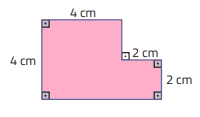
\includegraphics[width=1.65in,height=0.96458in]{./imgSAEB_8_MAT/media/image43.png}
\end{figure}

\reduline{$4 \cdot 4 + 2 \cdot 2 = A$\hfill}\\
\reduline{$16 + 4 = A$\hfill}\\
\reduline{$A = 20 cm^2$\hfill}
\item
\begin{figure}[H]
\centering
\includegraphics[width=1.50833in,height=1.28681in]{./imgSAEB_8_MAT/media/image44.png}
\end{figure}

\reduline{3 . 3 . 3\hfill}\\
\reduline{A = 27 centímetros quadrados\hfill}
\end{escolha}

\num{5} Para construir uma caixa com a forma de um bloco retangular sem
tampa, Rosangela recortou uma região poligonal de papelão, como esta
figura, e dobrou e colou com fita-crepe. Quantos centímetros quadrados de papelão ela
usou?

\begin{figure}[H]
\centering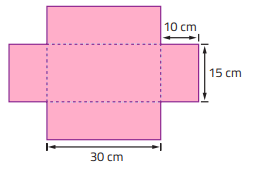
\includegraphics[width=1.98333in,height=1.33255in]{./imgSAEB_8_MAT/media/image45.png}
\end{figure}

\reduline{ Somando todas as áreas das figuras tracejadas, temos que:\hfill}\\
\reduline{ $10 \cdot 15 + 10 \cdot 15 + 10 \cdot 30 + 10 \cdot 30 + 15 \cdot 30 = A$\hfill}\\
\reduline{ $150 + 150 + 300 + 300 + 450 = A$\hfill}\\
\reduline{ $A = 1.350 cm^2$\hfill}\\

\pagebreak

\num{6} Determine a área das figuras a seguir.

\begin{escolha}
\item
\begin{figure}[H]
\centering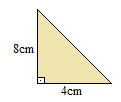
\includegraphics[width=1.26042in,height=1.0625in]{./imgSAEB_8_MAT/media/image46.png}
\end{figure}

\item
\begin{figure}[H]
\centering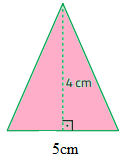
\includegraphics[width=1.39583in,height=1.72917in]{./imgSAEB_8_MAT/media/image47.png}
\end{figure}

\item
\begin{figure}[H]
\centering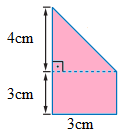
\includegraphics[width=1.375in,height=1.42708in]{./imgSAEB_8_MAT/media/image48.png}
\end{figure}

\item
\begin{figure}[H]
\centering\includegraphics[width=1.59375in,height=1.46875in]{./imgSAEB_8_MAT/media/image49.png}
\end{figure}
\end{escolha}

\reduline{a) $A = (\frac{4.8}{2})$\hfill}\\
\reduline{ $A = (\frac{32}{2})$\hfill}\\
\reduline{ $A = 16m^2$\hfill}\\
\reduline{b) A = $(\frac{\ 2,5.4}{2})$\hfill}\\
\reduline{A = $(\frac{10}{2})$\hfill}\\
\reduline{A = 5 + 5\hfill}\\
\reduline{A = 10 centímetros quadrados\hfill}\\
\reduline{c) A = $(\frac{12}{2})$\hfill}\\
\reduline{A = 6\hfill}\\
\reduline{6 + 9 = 15 centímetros quadrados\hfill}\\
\reduline{d) A = $(\frac{4.2}{2})$\hfill}\\
\reduline{ A = $(\frac{8}{2})$\hfill}\\
\reduline{ $A = 4$\hfill}\\
\reduline{ $4 + 4 + 8.5 = 48 cm^2$\hfill}\\

\num{7} Ao ler a bula de uma medicação, Andreia encontrou a seguinte
informação: ``Cada comprimido possui $x$ milímetros cúbicos dentro de sua cápsula''. Como
não conseguiu ler, pois a escrita estava rasurada, Andreia decidiu fazer
suas próprias medidas e obteve:

\begin{figure}[H]
\centering\includegraphics[width=1.88542in,height=1.3125in]{./imgSAEB_8_MAT/media/image50.png}
\end{figure}

Para saber o volume de medicação dentro da cápsula, qual fórmula Andreia deve utilizar?
Considerando-se (\Pi) = 3, qual é o volume da cápsula?

\reduline{ $V= (\Pi) \cdot R^2 \cdot h$\hfill}\\
\reduline{ $V = 3 \cdot 14 \cdot 11$\hfill}\\
\reduline{ $V = 462 mm^3$ de medicação.\hfill}\\

\pagebreak

\num{8} Calcule o volume do sólido a seguir.

\begin{figure}[H]
\centering\includegraphics[width=1.94792in,height=0.98958in]{./imgSAEB_8_MAT/media/image51.png}
\end{figure}

\reduline{ $V = l \cdot l \cdot l$\hfill}\\
\reduline{ $V = 8 \cdot 4 \cdot 3$\hfill}\\
\reduline{ $V = 96cm^3$\hfill}\\

\num{9} Calcule o volume do sólido a seguir.
\begin{figure}[H]
\centering\includegraphics[width=2.08333in,height=1in]{./imgSAEB_8_MAT/media/image52.png}
\end{figure}

\reduline{ $V = \frac{l \cdot l \cdot l}{2}$\hfill}\\
\reduline{ $V = \frac{4 \cdot 12 \cdot 3}{2}$\hfill}\\
\reduline{ $V = 72 cm^3$\hfill}\\

\num{10} Calcule o volume do sólido a seguir.

\begin{figure}[H]
\centering\includegraphics[width=1.92708in,height=1.5625in]{./imgSAEB_8_MAT/media/image53.png}
\end{figure}

\reduline{ $V_1 = 20 \cdot 10 \cdot 15 = 3.000$\hfill}\\
\reduline{ $V_2 = 15. 10 .10 = 1.500$\hfill}\\
\reduline{ $V_t = 1.500 + 3.000 = 4.500 cm^3$\hfill}\\

\num{11} Marina Resolveu colocar em sua casa uma piscina de 8 metros de
largura, 5 metros de comprimento e 1,5 metros de profundidade. Sabendo
que a companhia de água cobra 0,05 centavos por litro consumido, quantos
reais marina vai gastar para encher completamente essa piscina?

\reduline{ $V = 8 \cdot 5 \cdot 1,5 = 60 m^3$\hfill}\\
\reduline{ $60 m^3 = 60 000 litros \cdot 0,20 centavos$\hfill}\\
\reduline{ $12.000 centavos ou R\$\,120,00$\hfill}\\

\num{12} O reservatório de tinta de uma caneta comum tem a forma de um
cilindro. O diâmetro dele tem medida de comprimento de 3 mm e tem 14 cm
de medida de comprimento. Quantos mililitros de tinta essa caneta pode
acomodar? Considere (\Pi) = 3,14.

\reduline{ $V= (\Pi) \cdot R^2 .h$\hfill}\\
\reduline{ $V= 3,14 \cdot 1,5^2 \cdot 140$\hfill}\\
\reduline{ $V= 3,14 \cdot 2,25 \cdot 140$\hfill}\\
\reduline{ $V= 989,1 mm^3$\hfill}\\

\pagebreak

\section{Treino}

\num{1} Um cano cilíndrico de plástico tem 70 cm de medida de comprimento e
raio de 6 cm. Qual é a medida de volume que esse cano comporta?
Considere $\pi = 3$.


\begin{escolha}[itemsep=0pt]
\item 7.560.
\item 8.540.
\item 9.325.
\item 9.690.
\end{escolha}

% SAEB: Resolver problemas que envolvam volume de prismas retos ou
% cilindros retos.

% BNCC: EF08MA20 -- Reconhecer a relação entre um litro e um decímetro
% cúbico e a relação entre litro e metro cúbico, para resolver problemas
% de cálculo de capacidade de recipientes.

% A: Correta, pois:

% V = (\Pi) \cdot R^2 .h

% V = 3 \cdot 6^2 \cdot 70

% V = 3 \cdot 36 \cdot 70

% V = 7.560 cm^3

% B: Incorreta, pois o aluno chegaria a esse valor utilizando a formula da
% área, e não a formula do volume como o enunciado pede.

% C: Incorreta, pois o aluno chegaria a esse valor calculando o perímetro
% da circunferência do cano, e não o volume como pede o enunciado.

% D: Incorreta, pois o aluno chegaria a esse valor ao esquecer o termo
% quadrático.

\num{2} Vanessa estava pintando um quadro em uma tela retangular de 1 m por
70 cm. Começou desenhando e colorindo com tinta amarela um losango de
diagonais 70 cm e 50 cm. No restante do quadro, Vanessa pretende colorir
de tinta verde. Qual é a área do quadro que falta ser pintada?

\begin{figure}[H]
\centering\includegraphics[width=2.95833in,height=1.56526in]{./imgSAEB_8_MAT/media/image54.png}
\end{figure}

\begin{escolha}[itemsep=0pt]
\item $5.250 cm^2$
\item $7.000 cm^2$
\item $1.750 cm^2$
\item $1.680 cm^2$
\end{escolha}

% SAEB: Resolver problemas que envolvam volume de prismas retos ou
% cilindros retos.

% BNCC: EF08MA19 -- Resolver e elaborar problemas que envolvam medidas de
% área de figuras geométricas, utilizando expressões de cálculo de área
% (quadriláteros, triângulos e círculos), em situações como determinar
% medida de terrenos.

% A: Correta, pois:

% Utilizando a fórmula da área do losango, temos que:

% A = (\frac{\text{D\ .\ d}}{2})=

% A = (\frac{70\ .\ 50}{2})=

% A = (\frac{3500}{2})

% A = 1.750 cm^2

% Calculando a área do retângulo, temos que:

% A = 100 \cdot 70

% A = 7.000 cm^2

% Subtraindo

% 7.000 - 1.750 = 5.250 cm^2

% B: Incorreta, pois este valor é referente apenas ao valor da área do
% retângulo do quadro.

% C: Incorreta, pois este valor é referente apenas à área que já foi
% pintada.

% D: Incorreta, pois o aluno chegaria nesse valor ao não converter o valor
% em metros para centímetros.

\num{3} Um condomínio resolveu trocar sua caixa d'água e colocar uma nova de
formato cilíndrico com diâmetro de base de comprimento 8 m e altura de
comprimento de 5 m.

Qual é o volume dessa nova caixa d'água? Considere $(\Pi) = 3,1$.

\begin{escolha}[itemsep=0pt]
\item $49,6 m^3$
\item $24,8 m^3$
\item $62 m^3$
\item $248 m^3$
\end{escolha}

% SAEB: Resolver problemas que envolvam volume de prismas retos ou
% cilindros retos.

% BNCC: EF08MA20 -- Reconhecer a relação entre um litro e um decímetro
% cúbico e a relação entre litro e metro cúbico, para resolver problemas
% de cálculo de capacidade de recipientes.

% A: Incorreta, pois o aluno poderia chegar a esse valor utilizando
% erroneamente a formula da área da base.

% B: Incorreta, pois o aluno poderia chegar a esse valor calculando o
% perímetro da base.

% C: Incorreta, pois o aluno poderia chegar a essa conclusão ao não
% observar o termo quadrático da fórmula.

% D: Correta, pois

% V= \Pi). R^2 .h

% V= 3,1 \cdot 4^2 \cdot 5

% V= 248 m^3

\chapter{Probabilidade}

\subsection{Habilidade SAEB  }

Resolver problemas que envolvam a probabilidade de
ocorrência de um resultado em eventos aleatórios equiprováveis
independentes ou dependentes.

\subsection{Habilidade da BNCC}

\begin{itemize}
  \item EF08MA22.
\end{itemize}

\conteudo{A probabilidade (P) de um evento (E) acontecer, a partir de um
experimento aleatório, é dada pela razão entre o número de elementos do
evento e o número de elementos do espaço amostral.

No estudo da probabilidade, um experimento é considerado aleatório se,
mesmo ao repeti-lo um número considerável de vezes, da mesma maneira, o
resultado obtido é imprevisível. O lançamento de um dado e o de uma
moeda são exemplos de experimentos aleatórios, pois em cada repetição do
experimento o resultado obtido não pode ser previsto.

Para cada experimento aleatório há um conjunto de possibilidades de
resultados.

Os subconjuntos do espaço amostral são denominados eventos. Se o
conjunto formado pelos elementos de um evento é vazio, dizemos que esse
evento é impossível. Quando o número de elementos do evento coincide com
o número de elementos do espaço amostral, o evento é chamado evento
certo.}

\pagebreak

\section{Atividades}

\num{1} Em um jogo de tabuleiro, Natali precisa tirar 4 no dado para
conseguir uma bonificação. Qual é a probabilidade de sair a face com o
número 4 em apenas um lançamento?

\reduline{ $(P(E)\frac{n(1)}{n(6)}).$\hfill}\\
\reduline{ Logo, a chance de Natali tirar o número 4 no dado\hfill}\\
\reduline{ e conseguir a bonificação é $(\frac{1}{6})$.\hfill}\\

\num{2} Marina está jogando bingo com suas amigas. Os números a serem
sorteados vão de 1 a 60. Qual é a probabilidade de o primeiro número 
sorteado ser:

\begin{escolha}[itemsep=0pt]
\item par.
\item ímpar.
\item primo.
\item múltiplo de 3.
\item múltiplo de 5.
\item maior que 50.
\item menor que 50.
\end{escolha}

\reduline{a) $(P(E)\frac{n(30)}{n(60)}) = (\frac{1}{2}) ou 50\%$.\hfill}\\
\reduline{b) $(P(E)\frac{n(30)}{n(60)}) = (\frac{1}{2}) ou 50\%$.\hfill}\\
\reduline{c) $(P(E)\frac{n(17)}{n(60)}) = (\frac{17}{60}) ou 28\%$, aproximadamente.\hfill}\\
\reduline{d) $(P(E)\frac{n(20)}{n(60)}) = (\frac{1}{3}) ou 33\%, $aproximadamente.\hfill}\\
\reduline{e) $(P(E)\frac{n(12)}{n(60)}) = (\frac{1}{5}) ou 20\%$.\hfill}\\
\reduline{f) $(P(E)\frac{n(10)}{n(60)}) = (\frac{1}{6}) ou 16\%$, aproximadamente.\hfill}\\
\reduline{g) $(P(E)\frac{n(49)}{n(60)}) = (\frac{49}{60}) ou 81\%$ aproximadamente.\hfill}

\num{3} Sidnei está jogando um jogo de cartas com seus amigos. Quatro cartas são
consideradas as mais fortes. Ao pegar uma carta do baralho, qual é a
chance de Sidnei tirar uma delas? Considere que o baralho tenha 52
cartas.

\reduline{P(E) = 4/52 = 1/13 = 7\% aproximadamente.\hfill}\\

\num{4} Gabriela, Carolina, Graziela, Leonardo e Cláudio são irmãos. Quantas são
as possibilidades de duplas formadas por eles?

\reduline{ $(\frac{5!}{3!.2!}) = (\frac{120}{6\ .\ 2})$\hfill}\\
\reduline{ $(\frac{120}{12}) = 10$ duplas podem ser formadas.\hfill}\\

\num{5} João e Maria estão jogando um jogo que consiste em lançar 2 moedas
para cima e observar seu resultado. Para João ganhar, ele precisa que
pelo menos uma delas tenha uma coroa como resultado. Qual é a
probabilidade de João vencer o jogo?

\reduline{ $(P(E)\frac{n(3)}{n(4)}) = (\frac{3}{4})$ ou $75\%$.\hfill}\\

\num{6} Um parque de diversões resolveu lançar uma promoção para seus
clientes e colocou uma urna contendo 1.200 bolinhas enumeradas de 1 a
1.200. Aquele que encontrasse uma bolinha com o número menor que 10
ganhava um prêmio. Qual é a probabilidade de alguém ganhar o prêmio em
uma chance?

\reduline{ $(P(E)\frac{n(9)}{n(1\ 200)})=(\frac{3}{400}) ou 0,75\%$\hfill}\\

\num{7} Regiane está indo para uma festa de casamento onde irá usar um
vestido, um sapato e um colar. Se ela dispõe de 8 vestidos, 12 sapatos e
3 colares para escolher, de quantos modos diferentes pode se vestir?

\reduline{ $12 \cdot 8 \cdot 3= 288$ maneiras diferentes.\hfill}\\

\num{8} Uma professora está montando um provão final para testar o
conhecimento de seus alunos. Ele contém 40 testes, cada um com quatro
alternativas, das quais apenas uma é correta. De quantas maneiras o
gabarito da prova pode ser montado?

\reduline{ 4 alternativas; 40 Questões\hfill}\\
\reduline{ Temos que $(4^{40})$\hfill}\\

\num{9} Rita é professora de uma sala de aula do 8°. ano com 40 alunos. Ao
fazer uma pesquisa, descobriu que 6 deles são canhotos. Certo dia, ela
decidiu sortear um livro para a classe. Qual é a probabilidade de um
aluno canhoto ganhar?

\reduline{$(P(E)\frac{n(6)}{n(40)}) = (\frac{3}{20}) = 15\%$.\hfill}\\

\num{10} Hilária é funcionária de uma empresa de telemarketing. Na última
semana do ano, haverá um sorteio para saber quem trabalhará em cada dia.
Sabendo disso, qual é a probabilidade de Hilária trabalhar no final de
semana? Considere o final de semana incluindo apenas sábado e domingo.

\reduline{$(P(E)\frac{n(2)}{n(7)}) = 28\%$, aproximadamente.\hfill}\\

\section{Treino}

\num{1} Em uma fábrica de sapatos, houve um defeito com umas das máquinas da
linha de produção. Após uma pesquisa realizada, foi constatado que, a
cada 100 pares produzidos, 4 pares apresentavam algum tipo de defeito.
Qual é a chance de encontrarmos um par defeituoso ao selecioná-lo
aleatoriamente?

\begin{escolha}[itemsep=0pt]
\item $40\%$
\item $1\%$
\item $4\%$
\item $25\%$
\end{escolha}

% SAEB: Resolver problemas que envolvam a probabilidade de ocorrência de
% um resultado em eventos aleatórios equiprováveis independentes ou
% dependentes

% BNCC: EF08MA22 -- Calcular a probabilidade de eventos, com base na
% construção do espaço amostral, utilizando o princípio multiplicativo, e
% reconhecer que a soma das probabilidades de todos os elementos do espaço
% amostral é igual a 1.

% A: Incorreta, pois, ao converter o valor em porcentagem erroneamente, o
% aluno chegaria a esse valor.

% B: Incorreta, pois esse valor seria o número de calçados a serem
% selecionados, e não a porcentagem final.

% C: Correta, pois:

% (P(E)\frac{n(4)}{n(100)}) = 0,04 ou 4\%

% D: Incorreta, pois o aluno poderia chegar a essa conclusão ao apenas
% dividir o número de calçados totais pelo número de pares.

\num{2} Em um restaurante de comida típica mineira, há diversas
possibilidades de cardápio. Você pode escolher 3 tipos diferentes de
guarnições, 4 tipos de carnes, 6 tipos de saladas e 5 tipos de massas.
Há quantas possibilidades diferentes de pratos?

\begin{escolha}[itemsep=0pt]
\item 18 possibilidades
\item 72 possibilidades
\item 60 possibilidades
\item 300 possibilidades
\end{escolha}

% SAEB: Resolver problemas que envolvam a probabilidade de ocorrência de
% um resultado em eventos aleatórios equiprováveis independentes ou
% dependentes

% BNCC: EF08MA22 -- Calcular a probabilidade de eventos, com base na
% construção do espaço amostral, utilizando o princípio multiplicativo, e
% reconhecer que a soma das probabilidades de todos os elementos do espaço
% amostral é igual a 1.

% A: Incorreta, pois o aluno pode realizar uma soma ao invés de uma
% multiplicação.

% b: Incorreta, pois o aluno chegará a esse valor caso esqueça do elemento
% ``massas''.

% c: Incorreta, pois o aluno chegará a esse valor caso esqueça do elemento
% ``saladas''.

% D: Correta, pois:

% Relendo o enunciado, temos que:

% 4 \cdot 6 \cdot 5 = 300

\num{3} Um casal decidiu inovar na escolha do nome de seu novo filho. Todas
as letras do alfabeto foram colocadas em um saquinho, sendo que a letra
que fosse sorteada seria a letra inicial do nome do bebê. Em um sorteio
em condições justas, qual é a chance, aproximadamente, do filho do casal
ter a letra L como inicial do seu nome?

\begin{escolha}[itemsep=0pt]
\item $3\%$
\item $26\%$
\item $1\%$
\item $0,3\%$
\end{escolha}

% SAEB: Resolver problemas que envolvam a probabilidade de ocorrência de
% um resultado em eventos aleatórios equiprováveis independentes ou
% dependentes

% BNCC: EF08MA22 -- Calcular a probabilidade de eventos, com base na
% construção do espaço amostral, utilizando o princípio multiplicativo, e
% reconhecer que a soma das probabilidades de todos os elementos do espaço
% amostral é igual a 1.

% A: Correta, pois:

% (P(E)\frac{n(1)}{n(26)}) = 0,03 ou aproximadamente 3\%

% B: Incorreta, pois o aluno chegaria a essa conclusão ao confundir a
% quantidade de letras do alfabeto com a probabilidade do fato acontecer.

% C: Incorreta, pois o aluno chegaria a essa conclusão ao confundir a
% quantidade de iniciais com a probabilidade do fato acontecer.

% D: Incorreta, pois, ao deslocar a virgula uma casa para a direita, o
% aluno chegaria a essa resposta.